% Header mit Deklarationen
\documentclass[%
	pdftex,%              PDFTex verwenden
	a4paper,%             A4 Papier
	twoside,%             Einseitig/ wzeiseitig
	bibtotoc,%    		Literaturverzeichnis einfügen bibtotocnumbered: nummeriert
	liststotoc,%		Verzeichnisse einbinden in toc
	idxtotoc,%            Index ins Verzeichnis einfügen
	halfparskip,%        Europäischer Satz mit abstand zwischen Absätzen
	%chapterprefix,%       Kapitel anschreiben als Kapitel
	headsepline,%         Linie nach Kopfzeile
	footsepline,%         Linie vor Fusszeile
	pointlessnumbers,%     Nummern ohne abschließenden Punkt
	12pt,%                 Grössere Schrift, besser lesbar am bildschrim
	bibliography=totoc,
	cleardoublepage=empty,
	index=totoc,
	listof=totoc,
]{scrreprt}

%Maxi Biblio-Management
\usepackage[square,numbers]{natbib}
\bibliographystyle{unsrtdin}

%Zindath Biliothek Management
%\usepackage[backend=bibtex,bibencoding=ascii,style=numeric,citestyle=numeric-comp,defernumbers=true]{biblatex} 

%
% Seitenränder
%
\usepackage{geometry}
\geometry{a4paper, top=30mm, left=30mm, right=20mm, bottom=25mm, headsep=10mm, footskip=10mm}



%
% Paket für Übersetzungen ins Deutsche
%
\usepackage[french,english,ngerman]{babel}

%
% Pakete um Latin1 Zeichnensätze verwenden zu können und die dazu
% passenden Schriften.
%
%\usepackage[latin1]{inputenc}
% UTF8 Kompatabilität
\usepackage[utf8]{inputenc}
\usepackage[T1]{fontenc}

%
% Paket für Quotes
%
\usepackage[babel,french=guillemets,german=quotes]{csquotes}

%
% Paket zum Erweitern der Tabelleneigenschaften
%
\usepackage{array}


%
% Paket für schönere Tabellen
%
\usepackage{booktabs}

%
% Paket um Grafiken einbetten zu können
%
\usepackage{graphicx}
\usepackage{subfigure}
\usepackage{float} % zum abstellen der float umgebung von Grafiken
\usepackage[export]{adjustbox}

%
% Spezielle Schrift im Koma-Script setzen.
%
\setkomafont{sectioning}{\normalfont\bfseries}
\setkomafont{captionlabel}{\normalfont\bfseries} 
\setkomafont{pagehead}{\normalfont\bfseries} % Kopfzeilenschrift
\setkomafont{descriptionlabel}{\normalfont\bfseries}

%
% Zeilenumbruch bei Bildbeschreibungen.
%
\setcapindent{1em}
%\setlength{\abovecaptionskip}{0pt}

\usepackage{fancyhdr}
\pagestyle{fancy}
%\fancyhead{}
%\fancyfoot{}
%\fancyhead[LE,RO]{\leftmark}
%\fancyhead[LO]{\rightmark}
%\fancyhead[RE]{\thepage}
%\fancyhead[R]{\leftmark}
\fancyhead[RE]{\leftmark}
\fancyhead[LO]{\rightmark}
\fancyfoot[C]{\thepage}
\fancyhead[RO]{
\includegraphics[width=75pt]{Logos/HM_Deu_CMYK_Graust}}
\fancyhead[LE]{\textsc{Konstruktionsarbeit}}
\fancypagestyle{plain}{}
\renewcommand{\chaptermark}[1]{\markboth{\thechapter{} #1}{}}
\renewcommand{\sectionmark}[1]{\markright{\thesection{} #1}{}}
\setlength{\headheight}{37pt} 


%\usepackage{scrpage2}
%\pagestyle{scrheadings}
% Inhalt bis Section rechts und Chapter links
%\automark[section]{chapter}

% Mitte: leer
%\chead{}

%
% mathematische symbole aus dem AMS Paket.
%
\usepackage{amsmath}
\usepackage{amssymb}
\usepackage[fixamsmath, disallowspaces]{mathtools}

%
% Type 1 Fonts für bessere darstellung in PDF verwenden.
%
\usepackage{mathptmx}           % Times + passende Mathefonts
\usepackage[scaled=.92]{helvet} % skalierte Helvetica als \sfdefault
\usepackage{courier}            % Courier als \ttdefault

%
% Paket um Textteile drehen zu können
%
\usepackage{rotating}




%
%1 Glossaries / Verzeichnisse
%
\usepackage[nonumberlist,toc,nopostdot]{glossaries}
% Entferne alphabetische Gruppierung des Glossars
\renewcommand{\glsgroupskip}{}
\makeglossaries


%
% Paket um LIstings sauber zu formatieren.
%
\usepackage[savemem]{listings}
\lstloadlanguages{TeX}



%
% Neue Umgebungen
%
\newenvironment{ListChanges}%
	{\begin{list}{$\diamondsuit$}{}}%
	{\end{list}}

%
% aller Bilder werden im Unterverzeichnis figures gesucht:
%
\graphicspath{{bilder/}}


%
% Anführungsstriche mithilfe von \textss{-anzufuehrendes-}
%
\newcommand{\textss}[1]{"`#1"'}

%
% Strukturiertiefe bis subsubsection{} möglich
%
\setcounter{secnumdepth}{4}

%
% Dargestellte Strukturiertiefe im Inhaltsverzeichnis
%
\setcounter{tocdepth}{4}

%
% Zeilenabstand wird um den Faktor 1.5 verändert
%
%\renewcommand{\baselinestretch}{1.5}
\usepackage{setspace} %Zeilenabstand einstellbar



\usepackage{caption}


\DeclareUnicodeCharacter{00A0}{ }



\usepackage{verbatim}




%\newcommand{\submissiondate}{27. August 2015}
%\newcommand{\submissionmonthyear}{August 2015}


% Tabellenprogramm
\usepackage{tabularx}
\usepackage{multirow}

% Plotten von Tabellen
\usepackage[svgnames]{xcolor}
\usepackage{pgfplots}
\pgfplotsset{every axis/.append style={
thick,
tick style={thick}},
%width=10cm,
compat=1.12,
cycle list={Bihler1\\Bihler2\\green\\orange\\},
}
\usepgfplotslibrary{external}
\usetikzlibrary{pgfplots.groupplots}



\usepackage{siunitx}



\addto\captionsngerman{
\renewcommand{\figurename}{Abb.}
\renewcommand{\tablename}{Tab.}
%\renewcommand{\refname}{Quellenverzeichnis}
% \renewcommand{\bibname}{Quellenverzeichnis}
}




% Bihlerfarben
\definecolor{Bihler1}{RGB}{21, 78, 113}
\definecolor{Bihler2}{RGB}{146, 46, 46}




\usepackage[section]{placeins}

\usepackage{pdfpages}

\usepackage{lscape}


\usepackage{colortbl}






\usepackage{microtype}
%\overfullrule=2cm



\newcommand*\cleartoleftpage{%
  \clearpage
  \ifodd\value{page}\hbox{}\newpage\fi
}





\begin{comment}
%
% Paket für Links innerhalb des PDF Dokuments
%
\definecolor{LinkColor}{rgb}{0,0,0.5}
\usepackage[%
	pdftitle={Titel},% Titel der Diplomarbeit
	pdfauthor={Jens Schmelkus},% Autor(en)
	pdfcreator={LaTeX, LaTeX with hyperref and KOMA-Script},% Genutzte Programme
	pdfsubject={Diplomarbeit}, % Betreff
	pdfkeywords={Keywords}]{hyperref} % Keywords halt :-)
\hypersetup{colorlinks=false,% Definition der Links im PDF File
	linkcolor=LinkColor,%
	citecolor=LinkColor,%
	filecolor=LinkColor,%
	menucolor=LinkColor,%
	pagecolor=LinkColor,%
	urlcolor=LinkColor}
	
	
\definecolor{Colour1}{HTML}{1B9E77}
\definecolor{Colour2}{HTML}{D95F02}
\definecolor{Colour3}{HTML}{7570B3}
\definecolor{Colour4}{HTML}{E7298A}
\definecolor{Colour5}{HTML}{66A61E}
\definecolor{Colour6}{HTML}{E6AB02}
\definecolor{Colour7}{HTML}{A6761D}
\end{comment}


% Zinz Biblio-Management
% Literaturverzeichnis
% \bibliography{literatur/bib}

\begin{document}

% Römische Nummerierung für Sonderseiten, wie Verzeichnisse und Anhang
\pagenumbering{Roman}

% Titelblatt
\begin{titlepage}
\setcounter{page}{1}
%\thispagestyle {empty}
%\fancypagestyle{plain}{}
\begin{center}
%\vspace{2cm}
%\setlength{\headheight}{15pt}
\begin{figure}[h!]
\vspace{0cm}
\centering
% 
\includegraphics[width=0.6\textwidth]{graphics/HM_Deu_CMYK}

\includegraphics[width=0.8\textwidth]{bilder/Logos/FK03_CMYK_Block.png}
\\[0.8cm]
% \includegraphics[width=0.25\textwidth]{bilder/}
\end{figure}
\vspace{1.5cm}

{\fontsize{20}{60}\scshape Konstruktionsarbeit im vierten und Fünften Semester} 
\\[1.1cm]

\begin{doublespace}
{\fontsize{30}{22}\selectfont \textbf{Strukturauslegung eines Flügels für ein Kleinstflugzeug mit Lasten nach CS 23}\par} 
\vspace{1.4cm}
\end{doublespace}

\title{Vergleichende Strukturauslegung eines Flügels in Schalen und Rippenabuweise nach CS 23}
\author{Jens Schmelkus}
\date{Dezember 2017}

{\fontsize{23}{60}\scshape Jens Schmelkus} 
\\[2.0cm]


\textbf{Betreuer}: Prof. Dr. Guido Sperl



% \textbf{Fakultät}: Fakultät für Maschinenbau, Fahrzeugtechnik, Flugzeugtechnik

\textbf{Studiengang}: Fahrzeugtechnik 

\textbf{Abgabe}: 10.08.2018

\vfill


\end{center}
\end{titlepage}


\cleardoublepage\thispagestyle{empty}

% \chapter*{Eigenständigkeitserklärung}
% \markboth{Eigenständigkeitserklärung}{Eigenständigkeitserklärung}
\chapter*{Erklärung}\addcontentsline{toc}{chapter}{Erklärung}
\markboth{Erklärung}{Erklärung}

Hiermit wird erklärt, dass die Arbeit mit obigem Thema selbständig verfasst und noch nicht anderweitig für Prüfungszwecke vorgelegt wurde. Weiterhin sind keine anderen als die angegebenen Quellen oder Hilfsmittel verwendet und wörtliche sowie sinngemäße Zitate als solche gekennzeichnet worden. \\[2cm]
\begin{tabularx}{\textwidth}{lX}
 München, den \_\_\_\_\_\_\_\_\_\_\_\_\_\_\_\_\_\_\_\_ \hspace{10 mm} & \_\_\_\_\_\_\_\_\_\_\_\_\_\_\_\_\_ \\[0.2cm]
 & \hspace{5 mm} {\footnotesize Jens Schmelkus}
\end{tabularx}





\cleardoublepage

% % Die eidesstattliche Erklärung mit Unterschrift
\chapter*{Sperrvermerk}\addcontentsline{toc}{chapter}{Sperrvermerk}

Diese Diplomarbeit enthält vertrauliche Informationen. Sie darf nicht vervielfältigt oder auf elektronischem Weg verteilt werden. Einsichtnahme ist für einen Zeitraum von 5 Jahren ab Abgabe nur für Prüfungszwecke gestattet.




\clearpage

\chapter*{Zusammenfassung}\addcontentsline{toc}{chapter}{Zusammenfassung}

Das Labor für Systemtechnik Entwickelt, Produziert und betreibt seit 2010 im Rahmen sowohl von Studentischen als auch Forschungsprojekten verschiedene Unbemannte Flugsysteme.
Der Schwerpunkt liegt hier bei Automatisch gesteuerten Flächenflugzeugen.
Das Abfluggewicht liegt zwischen 2 und 15 kg ,sowie Spannweiten zwischen 1,5 m und 5 m.

-->> Hier kurze Erwähnung AUVSI 

-->> Komplexes System genötigt verschiedenste Elektronik für Antrieb Aktuierung/Lenkung Funkkontakt Energiemenagement etc.

-->> Dafür wird in dieser Arbeit ein Elektrisches Funktionskonzept erstellt und die Anforderungen Formuliert

-->> ES werden Baugruppen Entwickelt die die jeweiligen Subanforderunge erfüllen sollen

-->> Test von Subkompanenten (Ideale Diode)

-->> Elektronischer Gesamtaufbau entsteht und wird erklärt

-->> Elektronikerprobung wird beschrieben und Messdaten fezeigt (so.)

-->> Flugversuch Praxistest ---> Wettbewerbseinsatz und Wettbewerbsergebnis



\clearpage

% Verzeichnisse
% Kopfzeile links Kapitel, rechts leer
%\ihead{\leftmark}
%\ohead{}
%\input{Sonderseiten/verzeichnisse}

%
% Inhaltsverzeichnis
%
\tableofcontents \addcontentsline{toc}{chapter}{Inhaltsverzeichnis}%\pdfbookmark[0]{Inhaltsverzeichnis}{sumario_label_pdf}


%\chapter*{Nomenklatur}
%\markboth{Nomenklatur}{Nomenklatur}
\addcontentsline{toc}{chapter}{Nomenklatur}
%
% In diesem Abschnitt werden alle in diesem Dokument verwendeten Bezeichner beschrieben.

% Falls zur jeweiligen Größe kein Koordinatensystem gegeben ist, wird dieses als Index spezifiziert oder ist nicht zutreffend.

%\section*{Kleine lateinische Bezeichner}
%\vspace{0.2cm}\noindent
%\begin{tabularx}{\textwidth}{lX}
 %$a$ & Schallgeschwindigkeit\\
%\end{tabularx}
%\vspace{0.5cm}\noindent


\section*{Formelzeichen}

\begin{tabularx}{\textwidth}{lll}
\textbf{Symbol} & \textbf{Einheit} & \textbf{Beschreibung}\\
& & \\
$A$ & \si{\meter\squared} & Querschnittsfläche \\
$D$ & \si{\milli\meter} & Durchmesser \\
$f$ & \si{\hertz} & Frequenz \\
$f(z)$ & 1 & normiertes Bewegungsgesetz \\
$J$ & \si{\kilogram\meter\squared} & Massenträgheitsmoment \\
$k_\mathrm{v}$ & \si{\meter\squared} & Durchflussbeiwert  \\
$K_v$ & \si{\cubic\meter\per\hour} & Durchflussfaktor \\
$M$ & \si{\newton\meter} & Moment \\
$n$ & \si{1\per\minute} & Drehzahl \\
$p$ & \si{\milli\meter} & Spindelsteigung \\
$p$ & \si{\bar} & Druck \\
$Q$ & \si{\cubic\meter\per\hour} & Dichte \\
$s(\varphi)$ & \si{\milli\meter\per\radian} & Weg des Abtriebsgliedes (Übertragungsfunktion 0. Ordnung) \\
$S$ & \si{\milli\meter} & Gesamtweg des gerade geführten Abtriebsgliedes \\
$t$ & \si{\second} & Zeit \\
$z$ & 1 & normierter Drehwinkel eines Bewegungsabschnittes \\
$Z$ & 1 & Anzahl \\
$\zeta$ & 1 & Druckverlustbeiwert \\
$\rho$ & \si{\kilogram\per\liter} & Dichte \\
$\varphi$ & \si{\radian} & Drehwinkel des Kurvenkörpers \\
$\Phi_{ik}$ & \si{\radian} & Gesamtdrehwinkel des Kurvenkörpers im Abschnitt $ik$  \\
\end{tabularx}

\clearpage

\section*{Indizes}

\begin{tabularx}{\textwidth}{ll}
\textbf{Symbol} & \textbf{Beschreibung}\\
& \\
$A$ & Außenring \\
$G$ & Gewinderollentrieb \\
$I$ & Innenring \\
$ik$ & Nummerierung der Bewegungsabschnitte \\
$max$ & Maximal \\
$n$ & Drehzahl \\
$NCA$ & Auf das Numerical Controlled Aggregat bezogen \\
$Ring$ & Ringkontakt am Wälzkörper \\
$T$ & Teilkreis \\
$ue$ & Überrollfrequenz \\
$W$ & Wälzkörper \\
$WA$ & Wälzkörper \\
$zus$ & zusätzlich \\
\end{tabularx}



\begin{comment}

\vspace{0.2cm}\noindent
\begin{tabularx}{\textwidth}{lll}
Symbol & Einheit & Beschreibung\\
$t$ & \si{\second} & Zeit \\
$p$ & \si{\milli\meter} & Spindelsteigung \\
$f(z)$ &  & Normierte Übertragungsfunktion \\
$n$ & \si{1\per\minute} & Drehzahl des Hauptantriebs \\
$a$ & \si{1\per\second\squared} & Winkelbeschleunigung \\
$u_{max}$ & \si{1\per\minute} & Maximale Drehzahl des NCA's \\
$S_{ik}$ & \si{\milli\meter} & Gesamtweg des gerade geführten Abtriebsgliedes im Abschnitt $ik$ \\
$\omega_a = \dot{\phi}$ & \si{\radian\per\second} & Winkelgeschwindigkeit des Kurvenkörpers \\
$\Phi_{ik}$ &   & Gesamtdrehwinkel des Kurvenkörpers im Abschnitt $ik$  \\
$ik$ & \si{\radian} bzw. \si{\degree} & Nummerierung der Bewegungsabschnitte \\
$z$ & 1 & normierter Drehwinkel eines Bewegungsabschnittes \\
$\varphi$ & \si{\radian} bzw. \si{\degree} & Drehwinkel des Kurvenkörpers \\
$s(\varphi)$ & \si{\milli\meter\per\radian} & Weg des Abtriebsgliedes (Übertragungsfunktion 0. Ordnung) \\
$n_{max}$ & \si{1\per\minute} & Maximale Drehzahl der Maschine \\
\end{tabularx}



 

\colorbox{orange}{nicht Aktuell muss noch überarbeitet werden}


\end{comment}




%  $u_{max}$ in $\frac{\text{U}}{min}$
 
 
 % TODO: Indizes


%
% Abkürzungsverzeichnis
%
%%


\newacronym[plural=NCAs,firstplural=Numerical  Controlled  Aggregate]{NCA}{NCA}{Numerical Controlled Aggregat}
\newacronym{VC1}{VC 1}{Vari Control 1}
\newacronym{FFT}{FFT}{Fast Fourier Transformation}
\newacronym{HFFT}{HFFT}{Hüllkurven Fast Fourier Transformation}
\newacronym{NC}{NC}{Numerical Controlled}
\newacronym{CNC}{CNC}{Computerized Numerical Controlled}
\newacronym[plural=cM,firstplural=centiMorgans (cM)]{cM}{cM}{centiMorgan}
\newacronym{SPS}{SPS}{speicherprogrammierbare Steuerung}
%\printglossary[title={Abkürzungsverzeichnis},toctitle={Abkürzungsverzeichnis},type=\acronymtype,style=long]








% Merke mir die römische Seitenzahl in 'roemisch' und setzte Nummeriernung 

% auf arabisch für die eigentlichen Kapitel
\cleardoublepage

\newcounter{roemisch}
\setcounter{roemisch}{\value{page}}
\pagenumbering{arabic}

\chapter{Das AUVSI Projekt}\label{cha:Das AUVSI Projekt}

Studentsiches Projekt im Labor  bla blub

\section{(Geschichte und Hintergrund) Der AUVSI Wettbewerb}

\cite{AUVSIrules}

\cite{Meiling}

-->> siehe Meiling 

\section{(Geschichte HM Team - Profs und wichtige Personen nennen) Das Studentische AUVSI Team}

-->> ggf auch Meiling

*Bilder Raussuchen

\section{(Geschichte und Hintergrund) Ecuador-Projekt}

\cite{Niclas}

\begin{figure}[H]
\centering
\includegraphics[width=0.9\textwidth]{bilder/Fotos/Ecuador_2015_Gruppenbild.jpg} 
\caption{Die Forschungsgruppe in Sharametsa} 
\label{Die Forschungsgruppe in Sharametsa}
\end{figure}


\section{(Entwicklungsgeschichte) Bisherige Flugzeuge}

Im laufe der Aktivität des UAV Projekts im Labor für Systemtechnik sind mit zunehmender Erfahrung verschiedenste Flugplattformen Betrieben worden. Die Bandbreite reicht von einfachen Modellflugzeugen bis hin zu vollständig Missionsangepassten Eigenkonstruktionen.
Dieser Abschnitt soll einen kurzen Überblick über diese Historie geben.

\begin{figure}[H]
\centering
\includegraphics[width=0.9\textwidth]{bilder/Fotos/Maya_2014.jpg} 
\caption{Erster Versuchsträger Modellflugzeug "Maja"} 
\label{Erster Versuchsträger Modellflugzeug "Maja"}
\end{figure}

Mit der eigentlich als Modellflugzeug erworbenen 'Maja' in Schaumbauweise wurden die ersten Gehversuche mit dem Ardupiloten und Telemetriesystemen im Flug unternommen. Das Knappe Platzangebot und die Moderaten Flugleistungen schränkten hier jedoch die Möglichkeiten stark ein. Auch war der Startvorgang ein nicht abzustellendes Problemfeld. Der Druckpropeller ermöglichte keinen sicheren Handstart und der Einsatz von Startwagen führte immer wieder zu Schäden.

\begin{figure}[H]
\centering
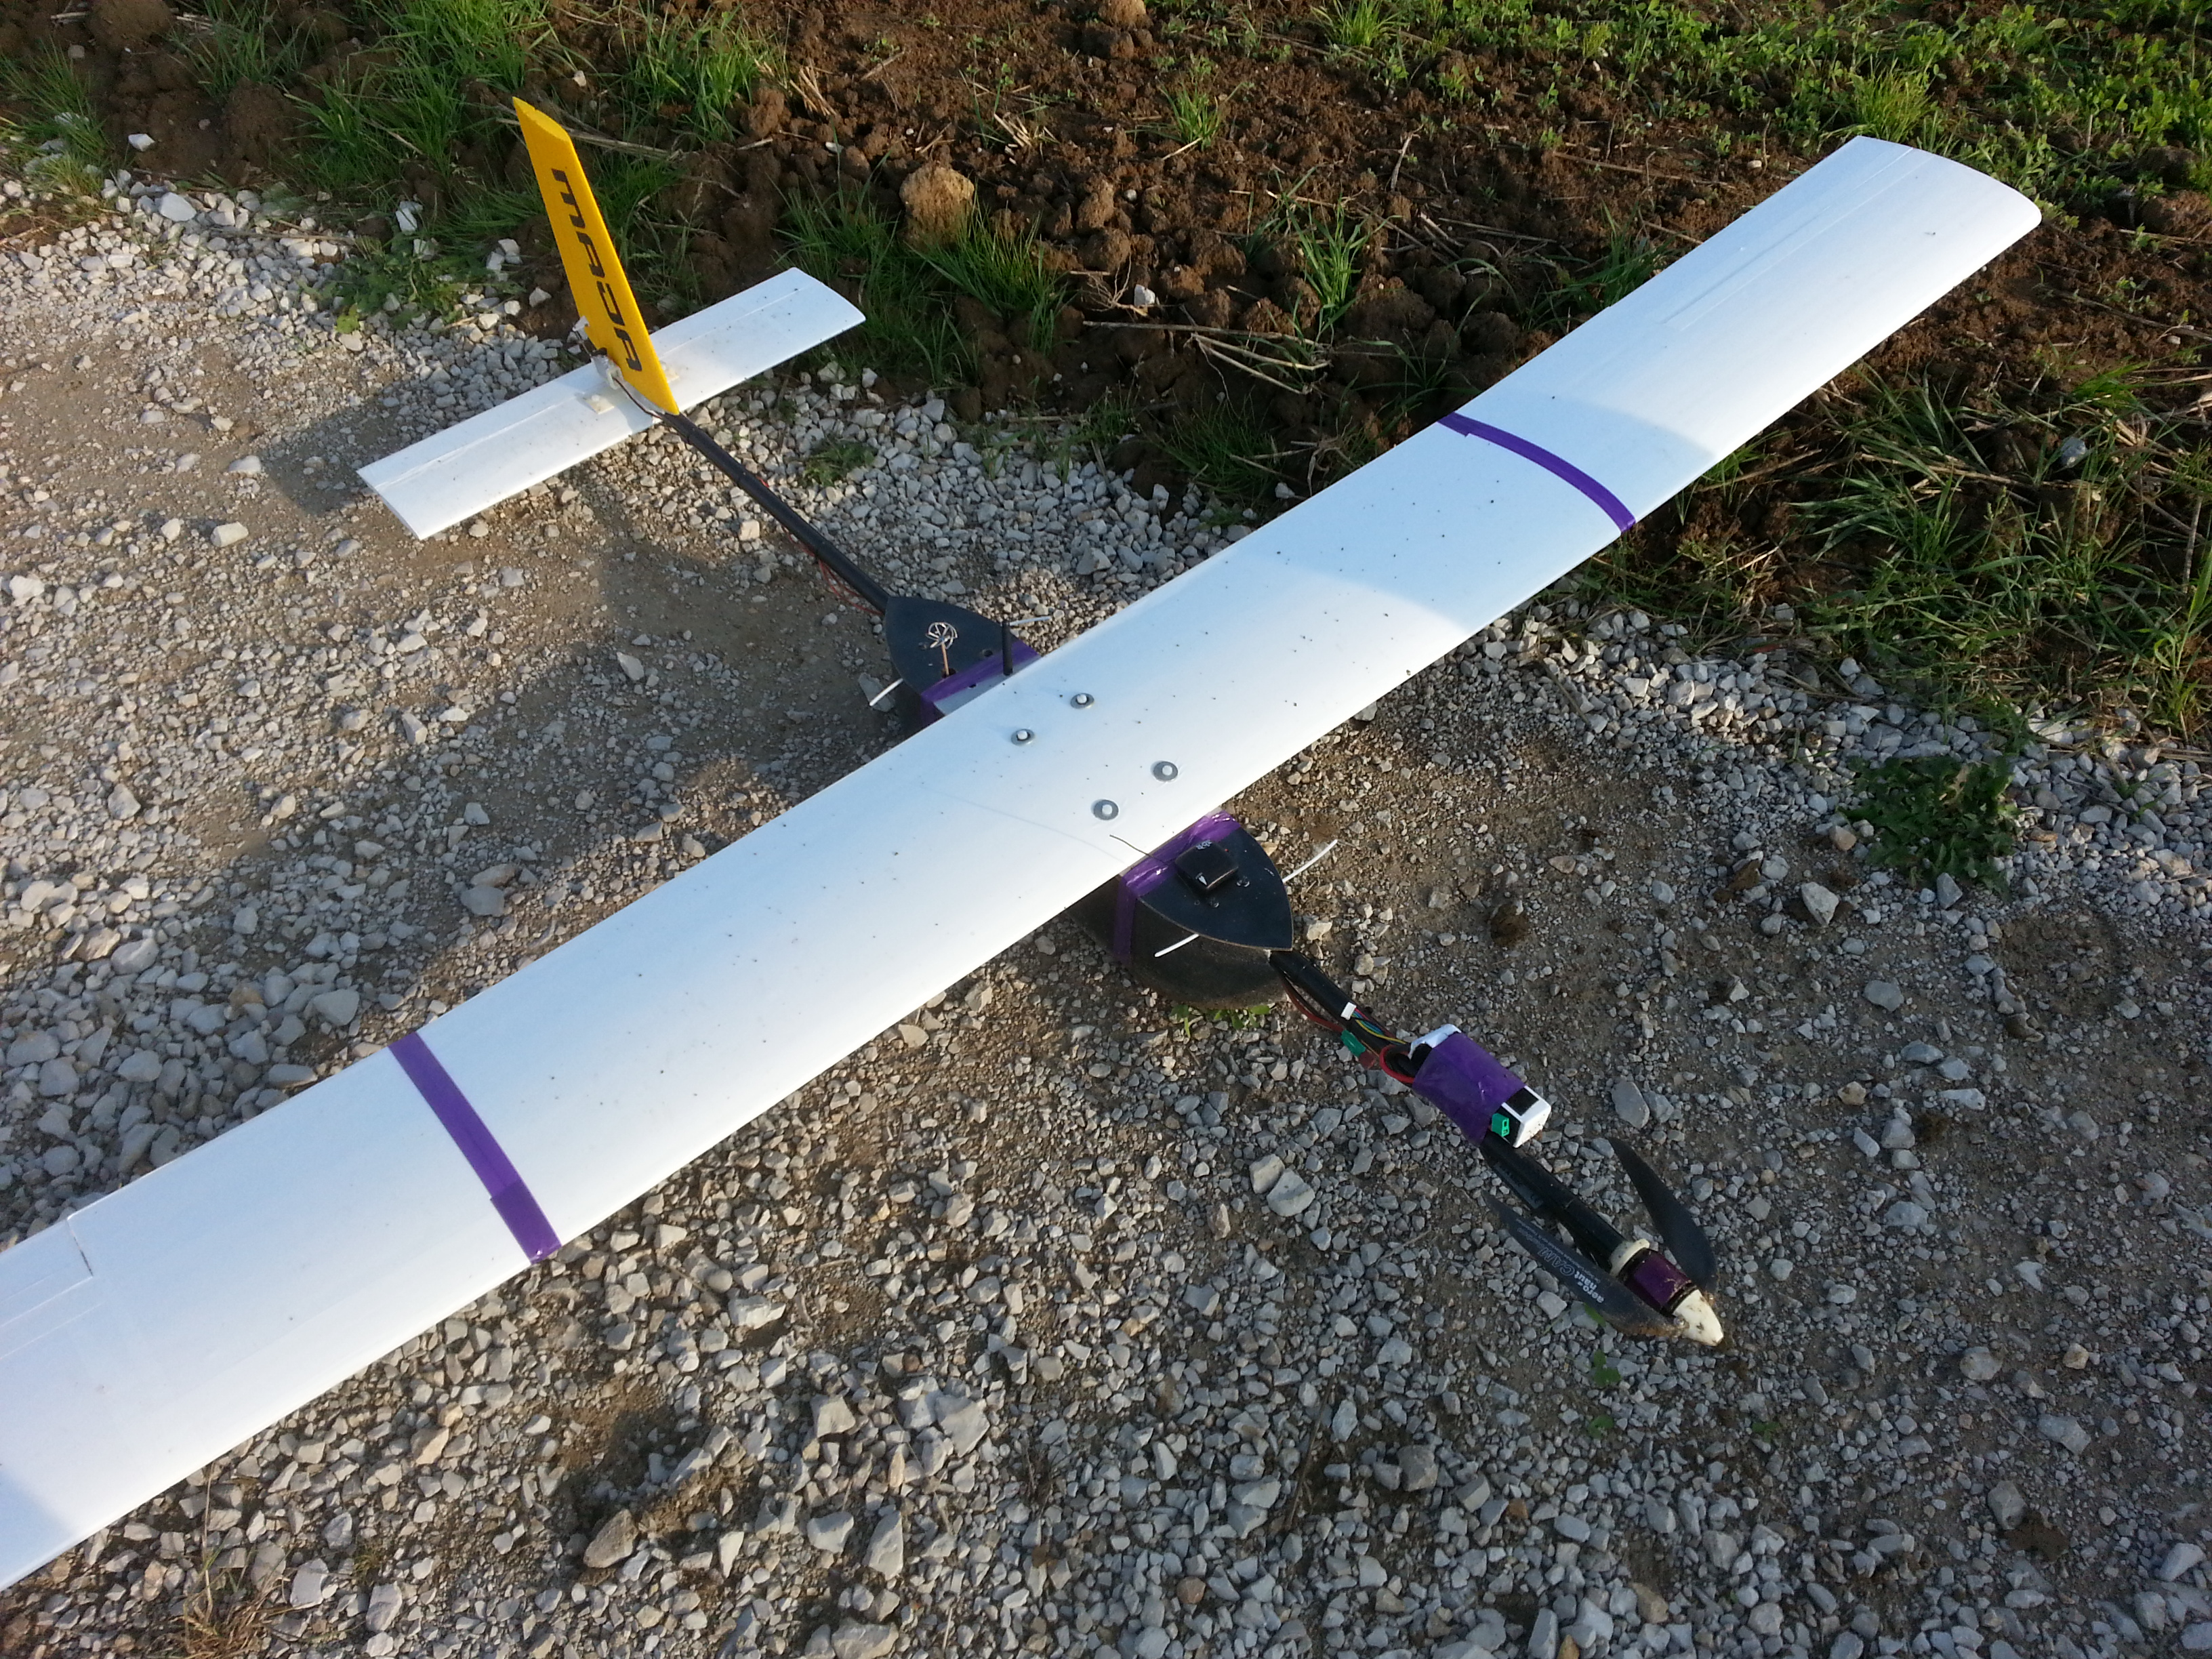
\includegraphics[width=0.9\textwidth]{bilder/Fotos/AUVSI-MAYA-Hybrid.jpg} 
\caption{Frühe Vorversuche für das AUVSI 2015 Flugzeug} 
\label{Frühe Vorversuche für das AUVSI 2015 Flugzeug}
\end{figure}

Daraus reiften das erste Konzept für einen selbst Konstruierten und Hergestellten Flieger. Die Flügel und Ruder waren in Klassischer Balsa beplankter Styroporbauweise ausgeführt die so bis heute im Einsatz ist. Erstmals war hier auch der Verfügbare Platz im Rumpfsegment an die Komponenten Angepasst. Während sich das neue Flugzeug an sich bewährte wurde der Rumpf als schlecht zu Handhaben und unzugänglich kritisiert.

\begin{figure}[H]
\centering
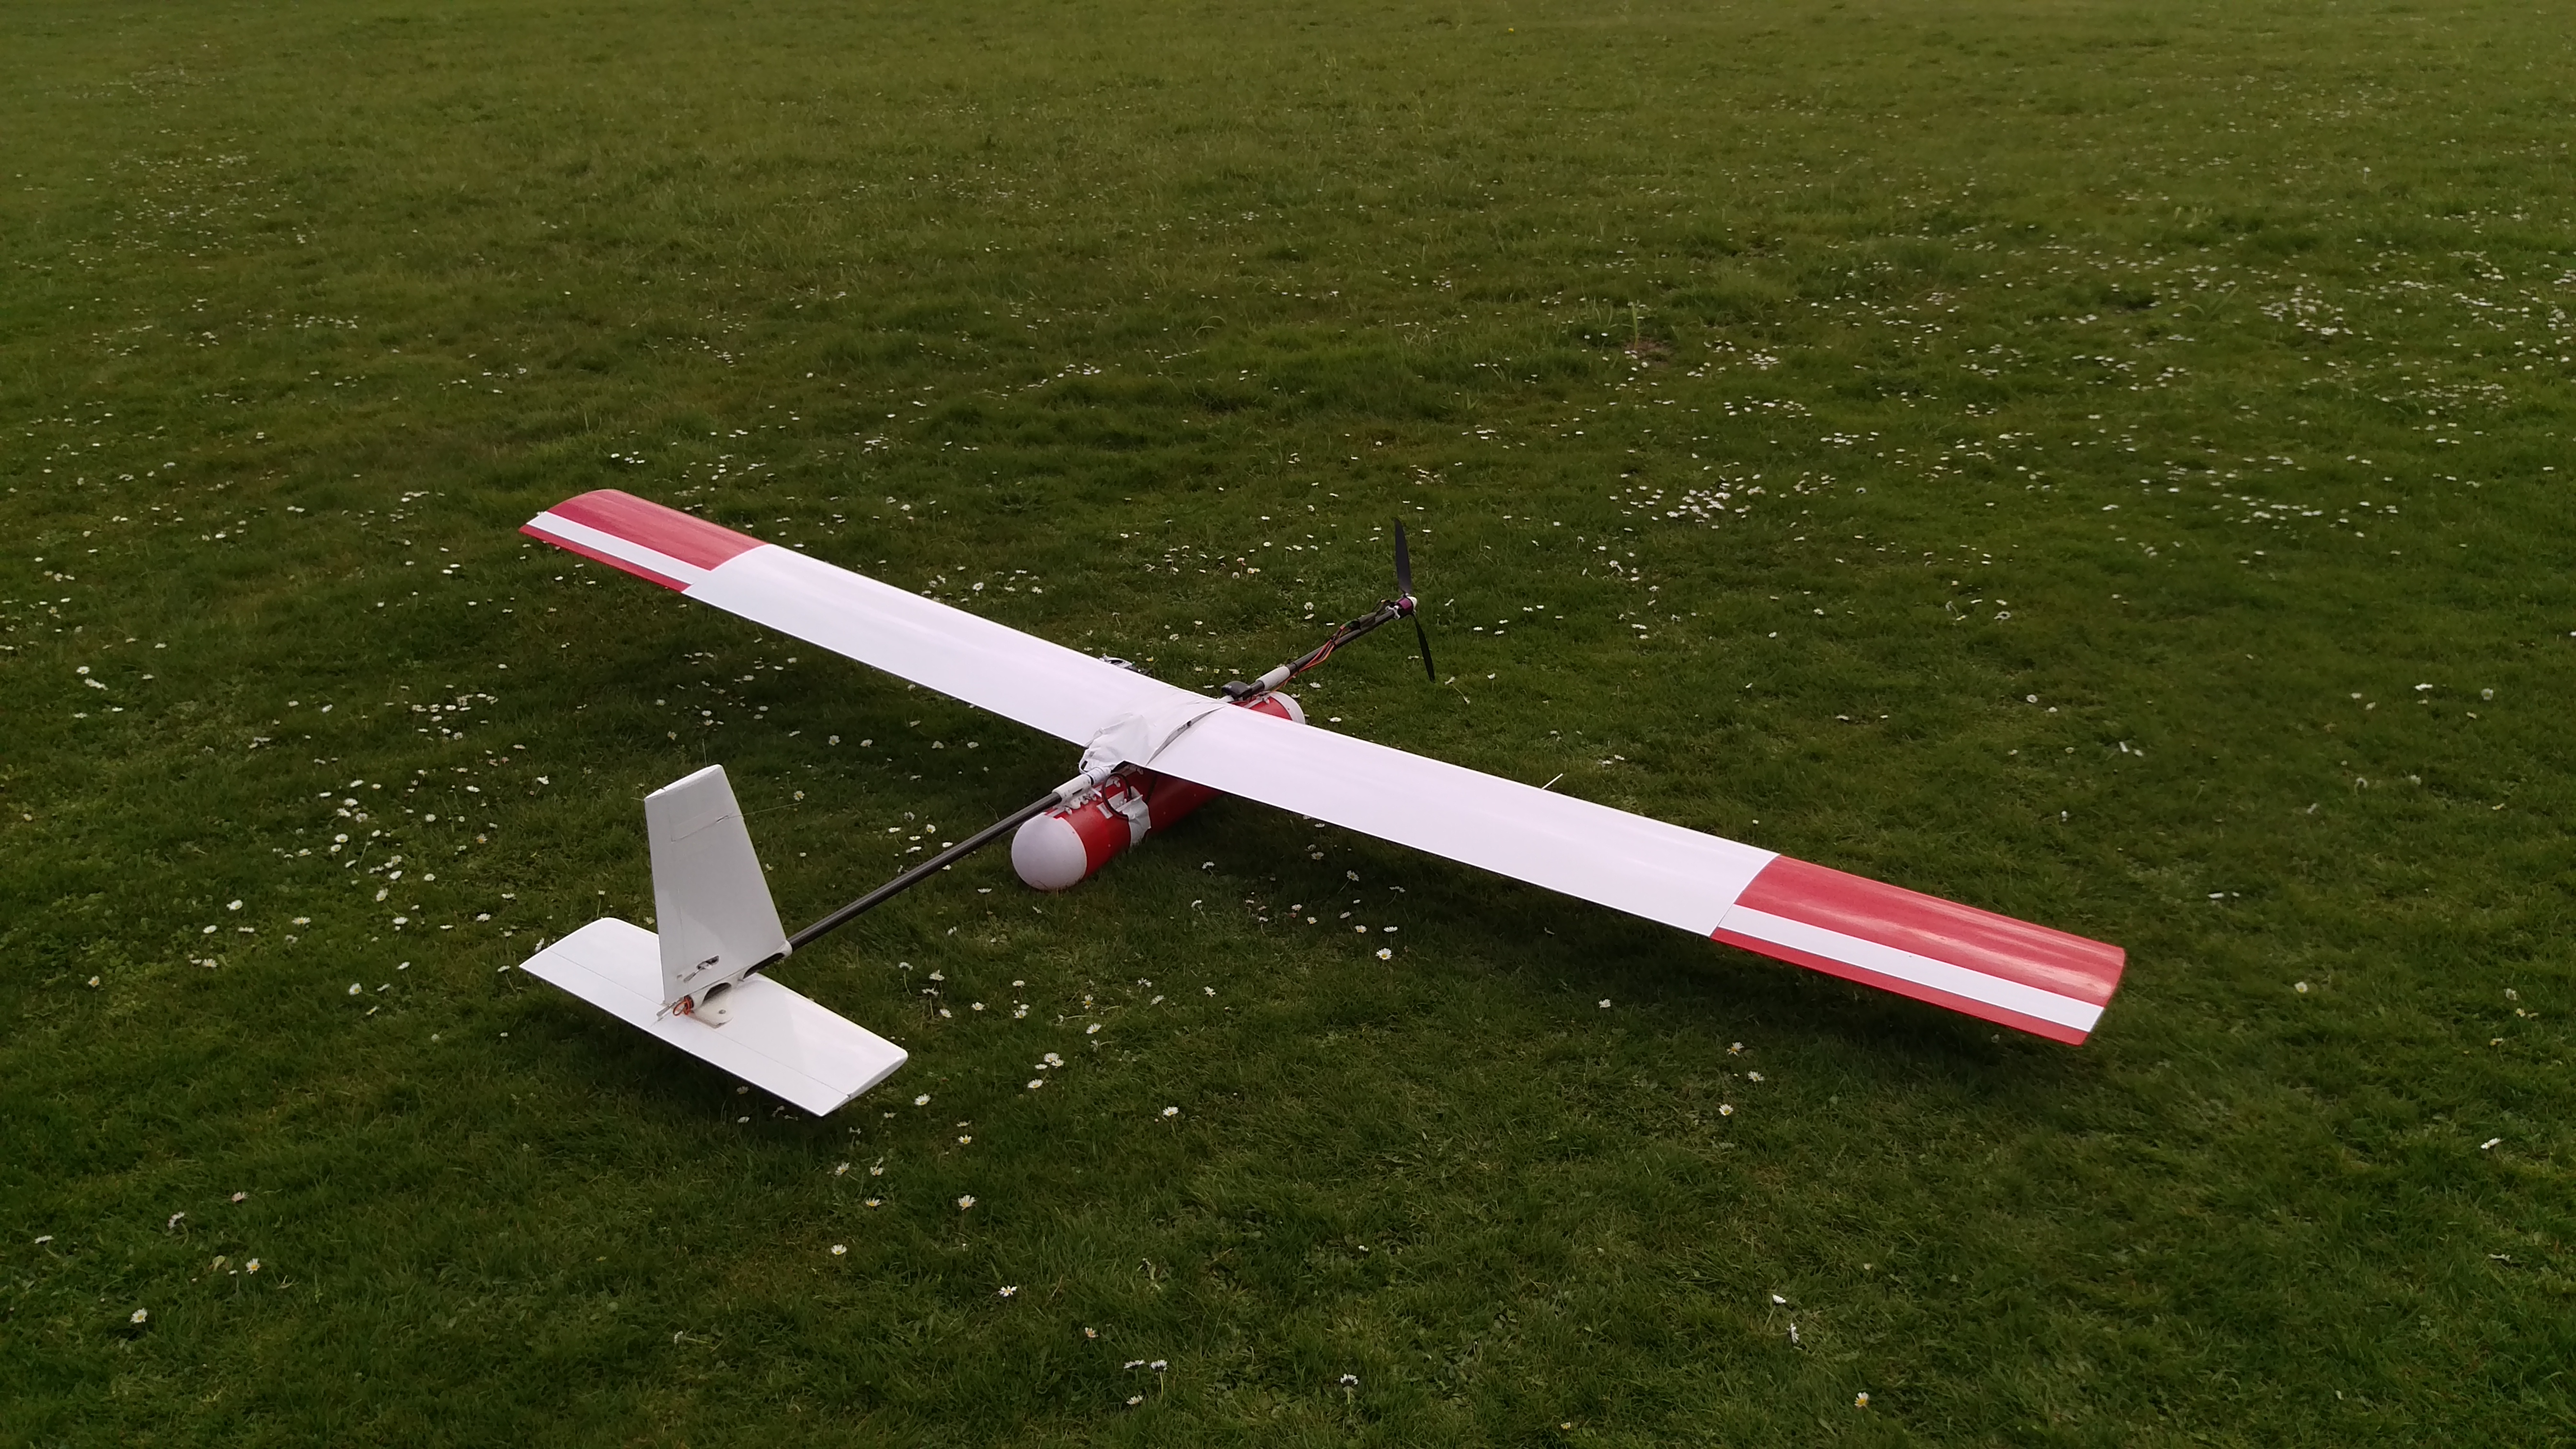
\includegraphics[width=0.9\textwidth]{bilder/Fotos/AUVSI_2015.jpg} 
\caption{Das AUVSI 2015 Modell in Einsatzzustand am Testflugplatz} 
\label{Das AUVSI 2015 Modell in Einsatzzustand am Testflugplatz}
\end{figure}

Damit entstand im Laufe der Arbeiten zur ersten eigenen Teilnahme am AUVSI Wettbewerb 2015 ein voll Modulares Hardware Konzept für Flügelkasten, Leitwerk, Leitwerksträger und Nutzlastrumpf.
Damit war eine gute Handhabung der einzelnen Sektionen bei Missionsvorbereitung und Modifikationen möglich. Integriert war hier auch die erste Generation einer eigenen Flugzeugbordelektronik für Leistungs und Signalpfade. Das auch über zahlreiche Testflüge gereifte Flugsystem konnte so auf dem Wettbewerb einen erfolgreichen siebten Platz erzielen.

\begin{figure}[H]
\centering
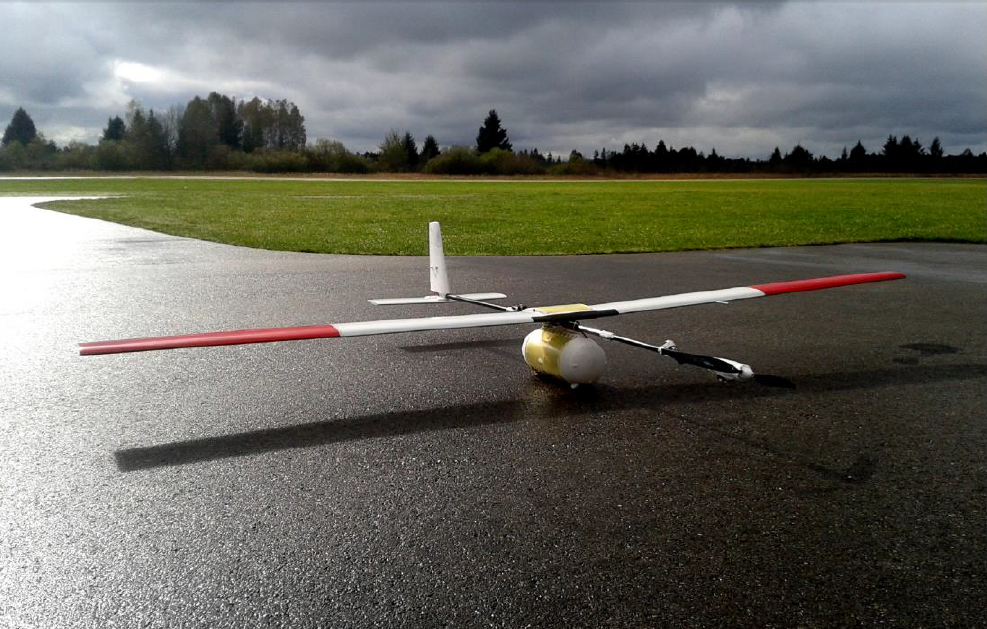
\includegraphics[width=0.9\textwidth]{bilder/Fotos/Ecuadorflieger_Koenigsdorf.png} 
\caption{Für die Fotomission in Ecuador modifizierter AUVSI 2015 Flieger in Königsdorf} 
\label{Für die Fotomission in Ecuador modifizierter AUVSI 2015 Flieger in Königsdorf}
\end{figure}

Im weiteren Verlauf des Jahres 2015 wurde das Forschungs Kooperationsprojekt mit der Fakultät für Geoinformatik in Angriff genommen. Die bewährte AUVSI 2015 Plattform wurde mit einem neuen Nutzlastrumpf nach dem Selben Modulprinzip ausgestatt der diesmal primär eine Hochauflösende Spiegelreflexkamara für Reihenbildaufnahmen trug. Es konnten zahlreiche routinierte Missionsflüge im Regenwald Ecuadors durchgeführt werden.

\begin{figure}[H]
\centering
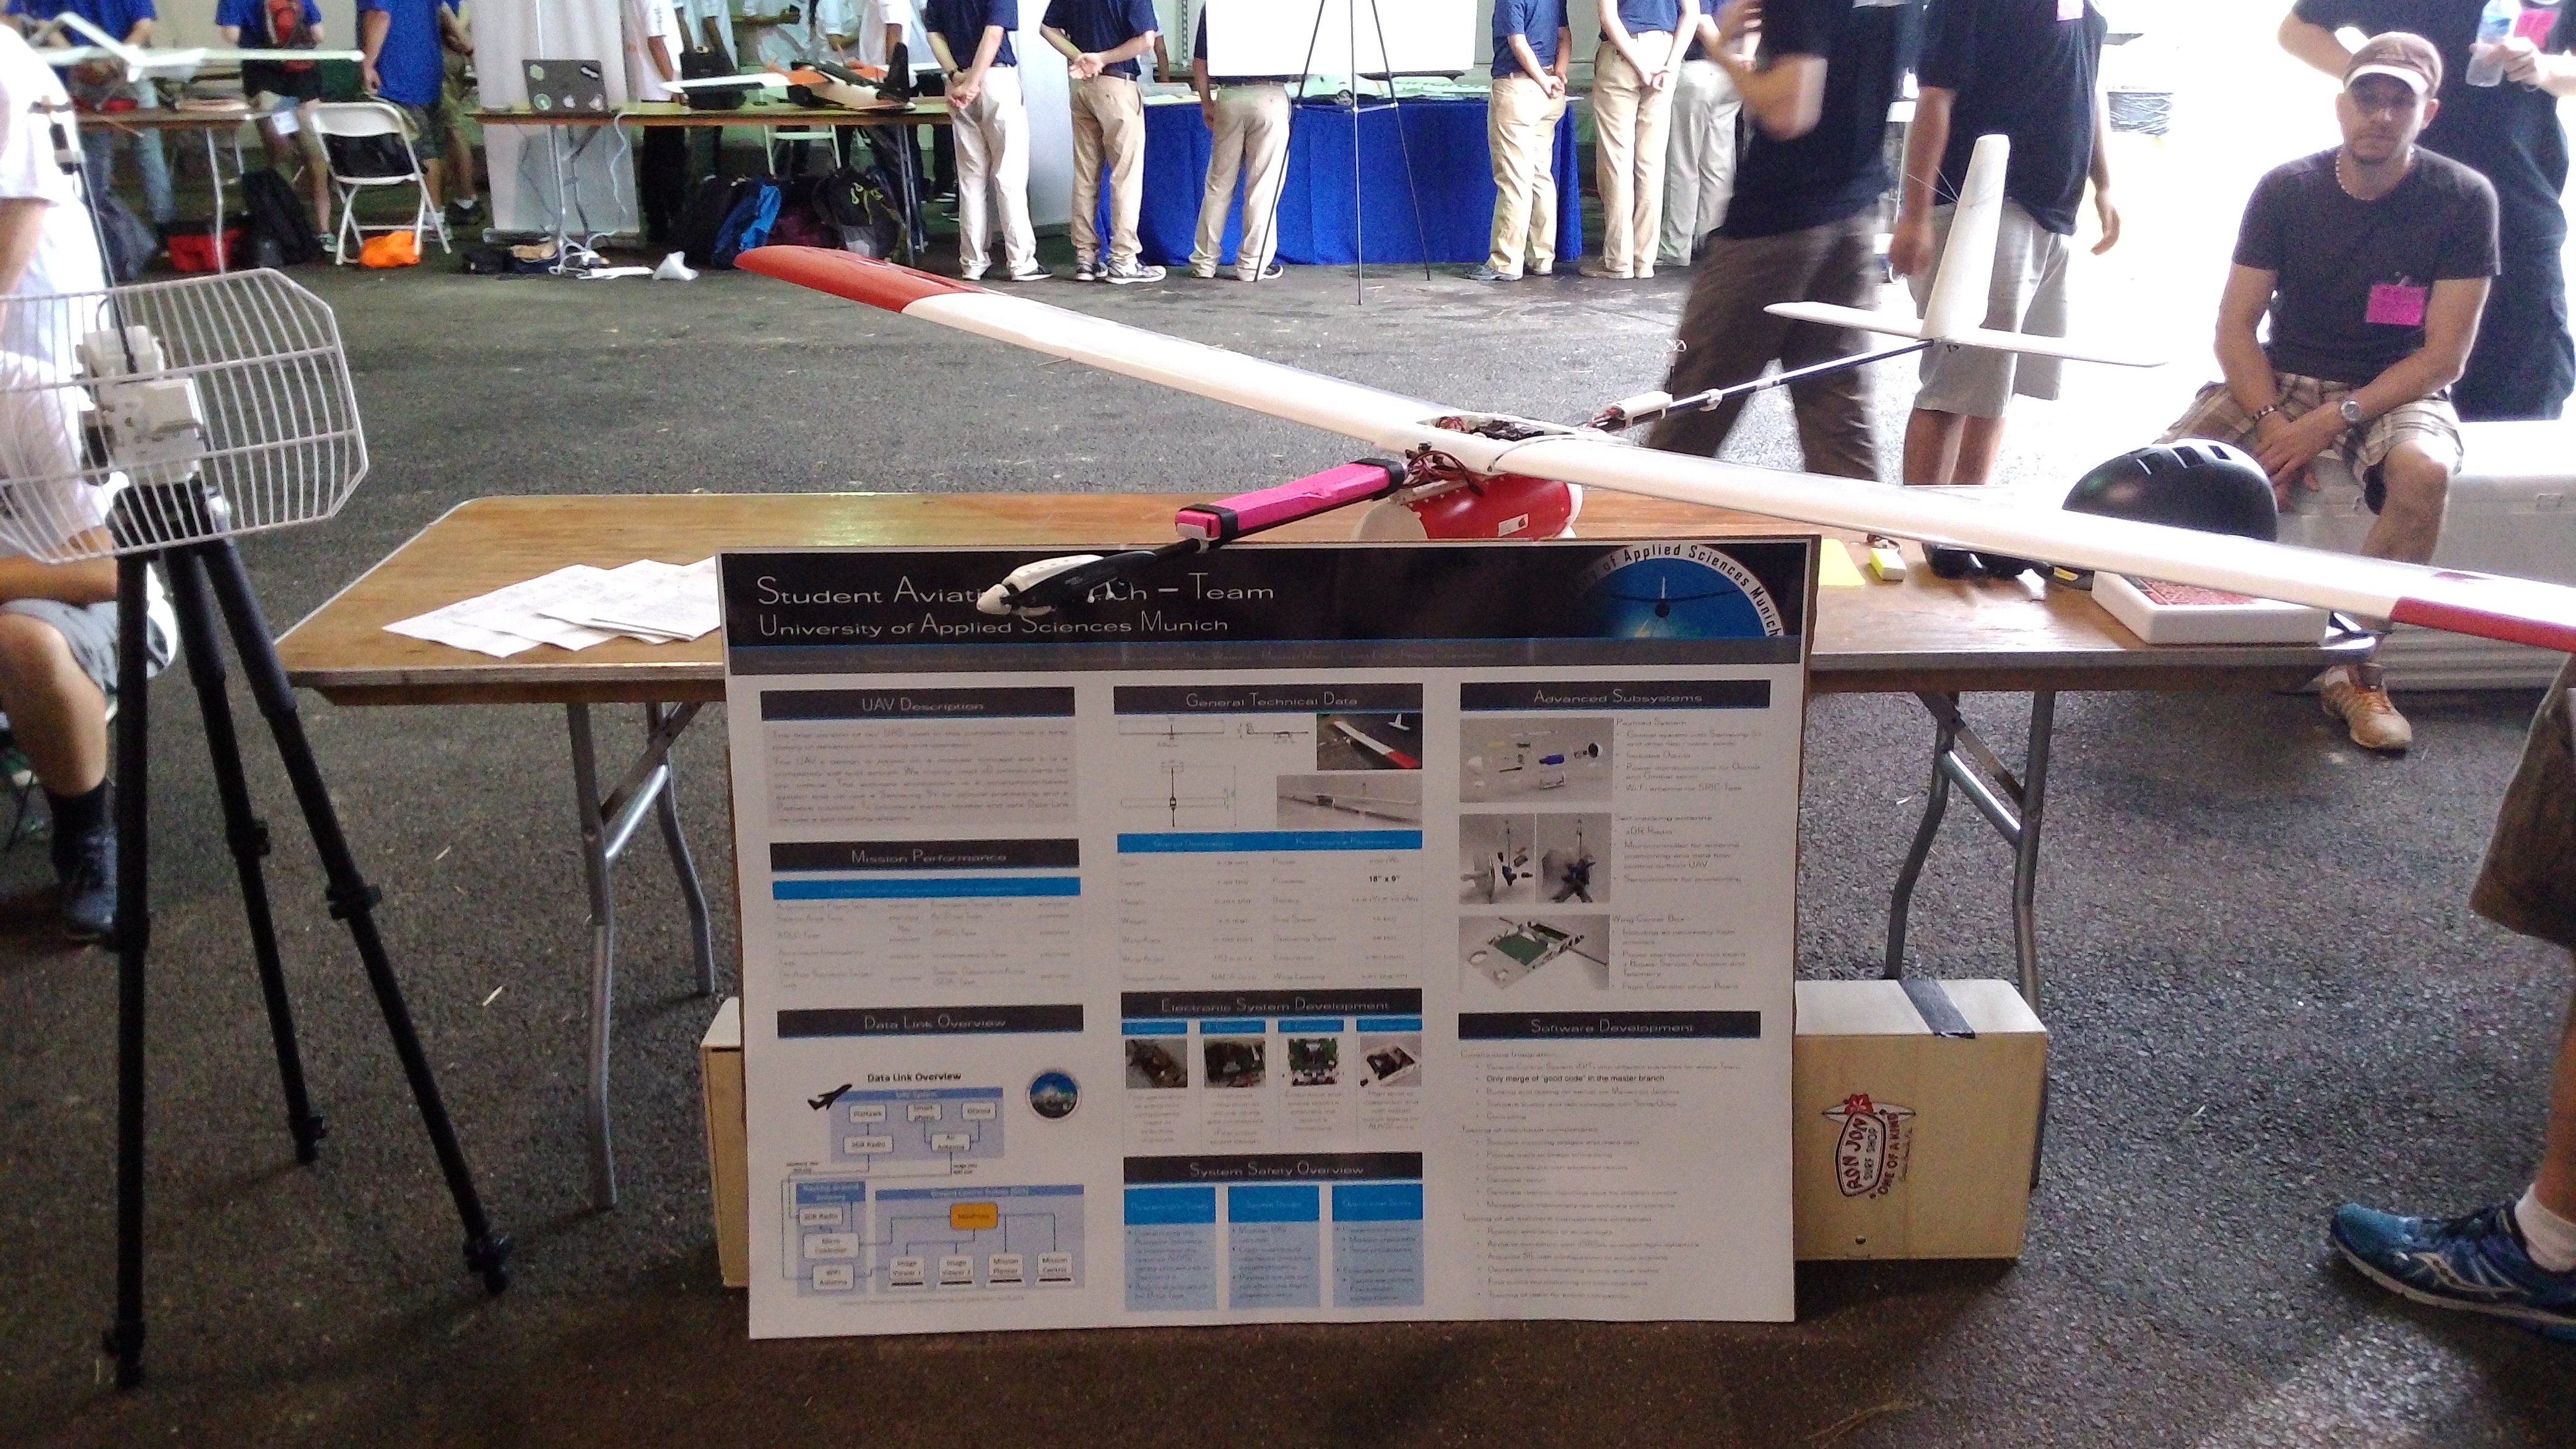
\includegraphics[width=0.9\textwidth]{bilder/Fotos/AUVSI_2016_Display.jpg} 
\caption{Der AUVSI 2016 Flieger beim Display auf dem Wettberwerb} 
\label{Der AUVSI 2016 Flieger beim Display auf dem Wettberwerb}
\end{figure}

Der AUVSI 2016 Flieger stellt eine konsequente Weiterentwicklung mit den Erfahrungen von AUVSI 2015 und der Ecuadormission dar. Erstmals wurden die Batterisysteme in die Flügel verlegt um Platz und mechanische Belastungen zu sparen. Eine neue Generation der Bordelektronik ermöglichte die Fremdversorgung der Missionsklaren Fliegers beim warten auf den Start. Die geänderten Anforderungen an Kamerasysteme und Bordcomputer konnten in einen deutlich Verkleinerten Rumpf umgesetzt werden. 

\cleardoublepage

\chapter{Anforderungen an die Flugplattform}\label{cha:Anforderungen an die Flugplattform}

Um eine zielgerichtete Entwicklung des Elektronikkonzepts zu ermöglichen wurden zunächst die globalen Anforderungen an die Flugplattform abstrakt formuliert. Diese wurden unter Einwirkungn des sich verändernden Reglements des AUVSI Wettberwerbs und die Formulierung neuer Aufgaben für die Flugplattform über die Einsatzdauer weiterentwickelt und ergänzt.  


\section{(Verändern) Anforderung an das Flugzeug}

Um einen sicheren Betrieb sowohl durch den Autopiloten als auch durch einen Menschlichen Testpiloten zur ermöglichen
wurde die Fluggeschwindigkeit zu Beginn zunächst auf maximal 18 m/s festgelegt. Die Geschwindigkeit am Punkt des Strömungsabsrisses wird Rechnerisch zu 10 m/s bestimmt.
Aus den Beschränkung beim Transport zum Wettbewerb als reguläres Gepäck im Internationalen Flugverkehr ergibt sich eine Maximale Länge aller Komponenten von 700 mm. Diese resultiert aus der größten Innenlänge der zur Verfügung stehenden Aluminium Transportkisten von etwa 725mm.
Aus Versicherungsrechtlichen Gründen wurde das maximale Startgewicht der Plattform auf 5 Kg beschränkt.
Es soll eine Ausreichende Operationsdauer für die Aufgaben des Wettbewerbs als auch andere Einsatzszenarien 
erreicht werden. Dabei müssen ausreichende Reserven für Sichtflug im Fehlerfall, Start, Steigflug und Landung vorgestehen werden.
Es wird damit eine Gesamtflugdauer von 45 Minuten als Szenario festgelegt.

Alle bestehenden Hubschrauber und Coptersysteme welche für ähnliche Aufgaben eingesetzt werden erzeugen Auftrieb ausschließlich aus Schub im Motor Propeller Antriebsstrang. Ein Flächenflugzeug wandelt den Schub auch bei kleinen Flügelstreckungen wenigstens im Verhältnis von 1:10 in Auftrieb um. Die Gleitzahl ist hier die Bestimmende Größe.

Damit fällt durch die Flugzeitvorgabe die Entscheidung für ein Flächenflugzeug. Anders erscheint diese Flugzeug bei Transport von Nutzlast unter Einhaltung des Abfluggewichts nicht realisierbar.

In dieser Arbeit soll keine Detaillierte Betrachtung der Aerodynamischen und Mechanischen Entwicklungsresultate für das Eigentliche Fluggerät stattfinden. Es wird festgehalten das alle bisher eingesetzten Flugzeuge die oben definierten Anforderungen erfüllen und Spannweiten zwischen 1,5 m und 2,8 m Aufweisen. Des weiteren wurden Abfluggewicht von 4 bis 4,9 Kg eingesetzt.


\section{(Verändern) Die Flugplattform als Sensorträger}

Um die zahlreichen Aufgaben des Wettbewerbs \begin{comment} Verweis auf Wettbewerbsaufben \end{comment}
erfüllen zu können muss die Flugplattform mit Sensoren und Verabreitungssystemen ausgestattet werden.
Zu diesen zählen hauptsächlich das Kamerasystem zur Detektierung der Buchstaben in der Suchaufgabe mit der dazugehören
Gimbal Vorrichtung zur Bildstabilisierung. Die Bilddaten sollen an Bord mit einem Kleinrechner  verarbeitet werden. Weitere Systeme sind der LIDAR Abstandssensor für einen akkuraten Landeanflug, sowie die Abwurfvorrichtung für das Ei beziehungsweise im späteren Regelwerk die Wasserflasche.
Es werden außerdem eine Reihe von Sensoren zur Versorgung des Autopiloten mit Flugdaten mitgeführt. Zu diesen zählen der GPS Empfänger, der Staudrucksensor sowie Batterie Strom- und Spannungssensoren.
Als Verbindung zur Bodenstation werden zwei Funkfrequenzen eingesetzt.
Eine 5 Ghz Wlan Verbindung welche eine Hohe Datenrate zur übertragung von Bildern  ermöglicht jedoch aufgrund der Frequenzchakrteristik am Bioden als gefgenstelle eine Nachgeführrte Richtantenne Erfordert.
Außerdem eine Dipolantenne im Frequenzbereich 433 Mhz welche zur übertragung der Flugdaten zwischen Autopilot und Bodenstation dient. Sie ermöglicht mit der Kleineren Frequenz eine größere Verbindungsreichweite bei gleicher Sendeleistung auf kosten den Datenrate.

Die Bildfrequenz der 2015 eingesetzten Kamera, Limitierte zunächst die Fluggeschwindigkeit im Reiseflug. Um eine für die weitere Auswerung der Bilder sinnvolle Überlappung von etwa 20 Prozent zu erzielen wurde die Geschwindigkeit auf 15 m/s gesetzt.

Die gesteigerte Bildfrequzenz und Auflösung des neusten Kamerasystems ermöglicht den Einsatz eine gesteigerten Missionsgeschwindikeit von 17 m/s welche für die Anwendung in der Saison 2018 geplant ist.

\section{(Ggf. Zusammenlegung mit folgendem Kapitel) Aufgaben der Elektronik}

Die Aufgaben der Elektronik lassen sich in den Bereich der Energieverwaltung und -verteilung  und den Bereich der Signalverteilung separieren.

Alle Subsystem sollen so gut wie möglich gegen Beschädigung durch Überlastung oder Fehlerhafter Bedienung geschützt werden.
Wenn möglich soll ein Kontrollierter Ausfall der Komponenten in bekannten Zustände realisiert werden.

Aus vorhergegangenen Test wurde das Flugsystem für eine Reine batterielektrische Versorgung Konzeptioniert.
Der Antrieb durch einen Verbrennungsmotor wurde für die Vorliegende Flugzeuggröße trotz besserem Energiegewicht als unzureichend zuverlässig, aufwendig handhabbar, sowie zu teuer eingestuft.
Des weiteren schränken bestehende Lärmschutzrichtlinien den Einsatz auf Testflugplätzen ein und es wird davon ausgegangen das sich die unvermeidbaren Vibrationen negativ auf die Zuverlässigkeit der Sensoren auswirkt.

\subsection{Energieverteilung und Verwaltung}

Die Elektrische Energie aus dem Akkusystem wird primär für die Erzeugung des Vortriebs über den Antriebstrang Motorregleer, Bürstenloser Motor, Getriebe und Luftschraube verwendet.
In diesem Pfand soll die Verwendung Mehrerer Quellen (Akkupacks) bei sicherer Handhabung ermöglicht werden.
Zweitgrößter Energieverbraucher sind die Aktorsysteme des Flugzeugs ("Servos") für alle Steuerflächen sowie Kamera (Gimbal) und Auswurfsysteme (Ei, Wasserflasche). Diese müssen mit einer festen Spannung von 5,0 Volt versorgt werden.
Drittgrößter Verbraucher an Bord sind die Funksysteme im 5 Ghz und 433 Mhz Band welche einer Festspannungsversorung mit 12 V  bedürfen.
Ebenfalls berücksichtigt werden sollen die Verbraucher des Sensorsystems, wie Kamera und Bordcomputer mit einer festen Spannung von 5,0 V hoher Qualität.
Als kleinster Verbraucher bedarf der Autopiloten Computer und seine Sensorsysteme eine Versorgung Hoher Genauigkeit sowie mit geringer Varianz mit 5,0 V.
Aus diesen wird innerhalb der Autopiloten Hardware selbstständig 3,3 V erzeugt.

Insgesamt sollen alle Subsysteme im Fehlerfall einen Reibungslosen Weiterbetrieb der restlichen Systemteilnehmer gewährleisten. Insbesondere der Aufrechterhaltung der Funktion des Autopilotensystems wird Priorität eingeräumt.


\subsection{Signalvertreilung}

Neben dem Pfad für die Energieverteilung bedürfen eine Vielzahl Logischer Signale der Verbindung und Verzweigung, sowie ausreichendem Schutz vor Fehlbedienung.

Primär erfolgt der Informationstransport über Digitale Bussysteme. Es kommen der I2C Bus, der SPI Bus, sowie serielle Verbindungen zum Einsatz.

I2C  Bus basierten Sensorsignalen gehören Systeme wie der Laser Höhenmesser LIDAR, Geschwindigkeitsmessung über Staudrucksonde sowie GPS zur Positionsbestimmung in Richtung der Eingänge des Autopilotensystems.

Die Kommunikation mit dem Funkübertragungssystem des Autopiloten erfolgt über einen Seriellen Bus.

Es besteht eine Verbindung vom Fernsteuerungsfunkempfängers und seines Satelliten mit dem Autpioloten.

Bisher basieren alle vom Autopiloten ausgegeben Steuersignale auf dem Prinzip der Pulsweitenmodulation "PWM"

Diese steuern den Motorkontroller, die Sonderfunktionen wie den Abwurfmechanismus sowie die Aktorsysteme desflugzeugs .


Die Eingänge des Autopiloten bedürfen eines Überspannungsschutzsystems für 3,3 V Logikspannung.

Die Ausgänge des Autopilotencomputers werden nicht speziell geschützt. Hier wird die Versorgung der Ausgänge des Autopiloten mit 5,0V bewerkstelligt. Diese liegt damit unter der  Maximalen Eingangsspannung der Verwendeten Aktorsysteme.


\section{(Verwirrend - Weitere Anforderungen Elektronik) Umsetzung in der Elektronik}

\subsection{Kabel und Steckersystem}

In erster Hardwareebene  wird der Schutz vor Beschädigung und Fehlbedienung der elektrischen Komponenten durch konservativ dimensionierten Einsatz von Kabeln und Steckersystemen erzielt. Die Kabelquerschnitte sind um
\begin{comment} Prozentzahl ?\end{comment}
überdimensioniert. Bei den Steckverbindungen wird nach Möglichkeit eine Einmalige Polanzahl des Verbinders gewählt.
Die Stecker besitzen bei empfindlichen Signalkabeln eine mechanische Arretierung durch virbationssicheren Formschluss in Form von Bügeln beziehungsweise Haken.
Um den Verschleiß der Kraftschluss basierten Signalstecker im Autopiloten zu vermeiden, werden alle Signale auf die Platine adaptiert und von dort mit Formschluss basierten Steckern weiter angeschlossen.

Die Leistungsverbinder im Hauptenergiepfad des Motors und der der Akkumulatoren sind Kraftschlussbasiert um einen Kompromiss aus Baugröße, Handhabung und Bertriebssicherheit zu erzielen.

\subsection{Trennung von Signal und Leistungsplatine}

Die  Hochleistungskomponenten im Pfad von den Batterien zum Antriebsstrang werden auf einer von dem Autopiloten und den Signalpfaden räumlich getrennten Platine realisiert. Dies bringt eine Reihe von Vorteilen für das System und die Entwicklung mit sich.

Es ist eine bessere Austauschbarkeit, Weiterentwicklung und Reparatur für einzelne Komponenten möglich.
Die Schadenshäufigkeit und deren Folgen sind auf der Leistungsplatine größer und graviernder was einen häufigeren 
Austausch und Weiterentwicklung zur Fehlerkorretur nötig macht.

Der Einsatz verschiedener Fertigungstechniken auf der Leistungs- und der Autopilotenplatine wird vereinfacht.

Die räumliche Trennung verringert den Einfluss durch die Hohen Wechselnden Ströme verursachten Elektrischen Felder auf das Empfindliche Autopilotensystem und seine Ein- und Ausgangssignale.

Sonstige Signalpfade werden im Heck der Flugzeugs zu GPS Empfänger und Antennensystem verlegt um einen größtmöglichen Abstand zur Leistungsplatine zu gewährleisten.

\subsection{Schutz des Batteriesystems}

Zur Realisierung einer Variablen großen Reichweite bei guter Handhabung werden im Regelfall mehrere Akkupacks gleicher Zellenzahl und Kapazität eingesetzt.
In der Praxis ist es unvermeidlich das der Ladezustand zweier Akkupacks aufgrund von Bauteilstreuung und Handhabung nie identische ist und damit eine Spannungsdifferenz aufweist. Damit würde der Akku mit dem höheren Spannungsniveau sich über eine Niederohmige Verbindung ungebremst in den zweiten Akku bis zum Spannungsangleich entladen. Dies erfolgt mit  hohen strömen und Beschädigung beider Akkumulatoren bis hin zum möglichen Brand der Akkuzellen.
Um zu Vermeiden das dieser Ausgleich stattfindet wird ein System Implementiert welches nur einen Stromfluss von allen Angeschlossenen Akkumulatoren in Richtung der Verbraucher Ermöglicht.
Dieses System wird aufgrund seiner Funktionsweise als "ideale Diode" bezeichnet. Es besteht aus einem integrierten Schaltkreis welches einenen Halbleiterschalter (Metalloxidfeldeffekttransistor kurz MOSFET) regelt um einen Konstante Spannungsdifferenz zwischen Eingang und Ausgang dieser Schaltung zu halten.

\subsection{Bereitstellung der Versorgungspannungen}

Die Erzeugung der erforderlichen Versorgungsspannungen für alle Subsysteme erfolgt über den Einbau von Gleichstrom-Gleichstrom Wechselrichtern (kurz DC-DC Wandlern).
Diese erzeugen die nötigen Spannungen durch sogenannte "Step down"  Wandlung aus der Spannung des Batteriesystems.
Für Empfindliche Systeme wie den Autopiloten und die Sensoren werden die jeweiligen Spannungen durch die Verwendung von Linearreglern erzeugt welche eine hohe Genauigkeit, geringe Varianz und niedrige Restwelligkeit des erzielten Ausgangsspannungswertes gewährleisten.

Um im Fehlerfall eines Subsystems durch zum Beispiel Kurzschluss eine Beschädigung des Spannungsversorgungssystems durch Überstrom und den daraus Resultierenden Ausfall der Systemgruppe zu vermeiden wird jeder Verbraucher mit einer selbstrückstellenden Sicherung mit einem Nennstrom in der Größenordnung von 125 Prozent seines Datenstroms ausgestattet.
So wird bei einem Überstromfehler das Subsystem abgetrennt und der Weiterbetrieb der Versorgung nicht beeinträchtigt.


\subsection{Handhabung der Logiksignale}

Alle Bussysteme sowie Steuersignale werden nach Möglichkeit weit entfernt von Leistungspfaden geführt und mit kurzen Verbindungen realisiert.
Bussysteme wie I2C erhalten die nötigen Grundbeschaltungen mit Pull up Wiederständen.

Eingangsignale in den Autopiloten erhalten eine Eingangs Schutzbeschaltung welche mithilfe einer zener Diode und Vorwiederständen welche Überspannung Ableitet.

\cleardoublepage

\chapter{Fortschreitende Elektronikentwicklung}\label{cha:Elektronikentwicklung}

In diesem Kapitel der Arbeit wird die Umsetzung der diversen Konzept und Strukturanforderungen in Hardware betrachtet. Dabei werden hier ausgesuchte Beispiele aus mehreren Vergangenen Jahren Vorgestellt und Technisch erläutert.
Dabei wird die kontinuierlich Fortschreitende Implementierung von Erfahrung im Zusammenspiel mit dem Modularen Gesamtkonzept aufgezeigt.

\section{Ursprünglicher Elektronikzustand}

Die in der Saison 2014 begonnen Voruntersuchungen fanden mit dem Flugsystem 'Maya' statt.
Abseits von Strukturellen und Flugmechanischen Problemen war auch die Elektronik eine kontinuierliche Quelle von Fehlern und Ausfällen des Flugzeugs.
Dies war größtenteils auf die Mangelnde Erfahrung im Umgang mit einem System eines solchen Komplexitätgrades zurückzuführen.Aber auch eine noch unzureichende Ausstattung mit Werkzeug,  Testmöglichkeiten und Methoden in Kombination mit der Unübersichtlichen Kabelführung erschwerte die Fehlersuche.
Auch die ersten versuche mit einem selbst gebauten Flächenmodell waren mit ähnlichen Schwierigkeiten in der Elektronik behaftet.

\begin{figure}[H]
\centering
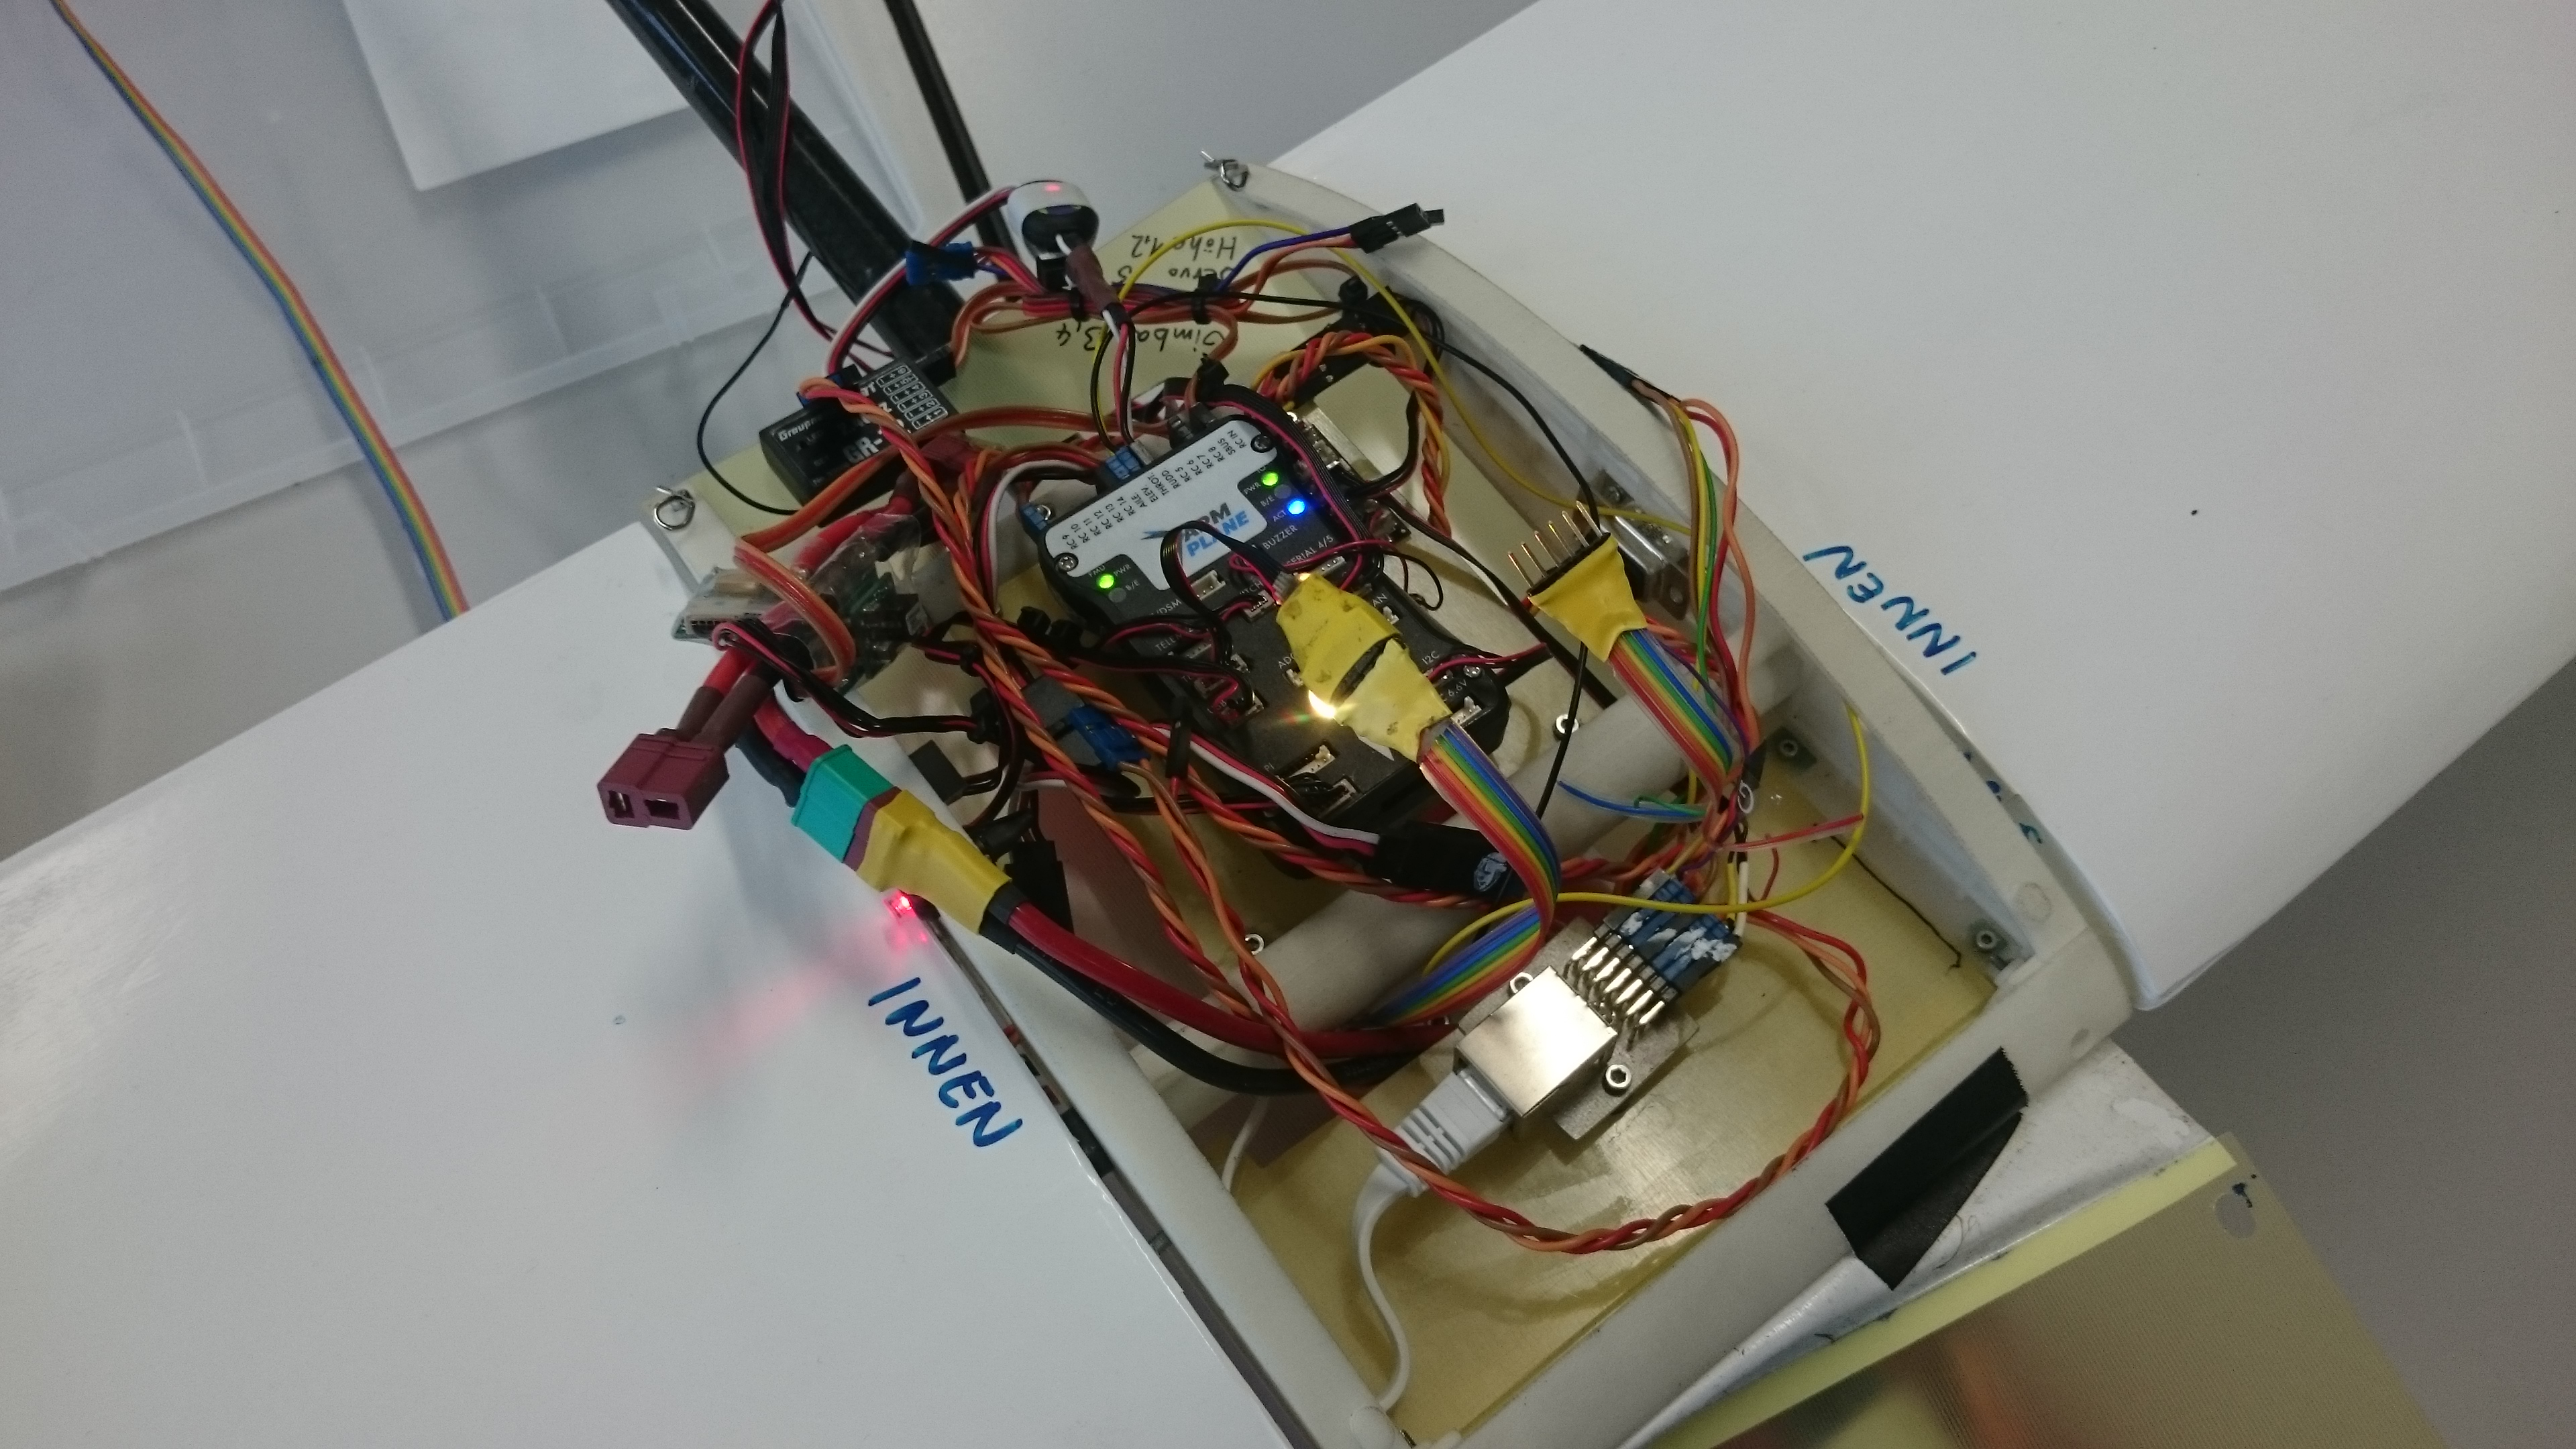
\includegraphics[width=0.9\textwidth]{bilder/Fotos/Elektronik_Kabelsalat_2015.jpg} 
\caption{Anblick der Elektronik zu Beginn 2015} 
\label{Anblick der Elektronik zu Beginn 2015}
\end{figure}

\section{Neue Platinenaufteilung}

Aus diesen Erfahrungen entstand das Eingangs vorgestellte Konzept für die Elektronik des Fliegers.
Dieses Konzept wurde 2015 erstmals angewandt, um eine Übersichtliche und einfach handhabbare Hardwareplattform mit leicht überprüfbaren Funktionen Umzusetzen.

Im Folgenden wird Beispielhaft die Bordelektronik des AUVSI 2016 Fliegers betrachtet.

\subsection{Leistungsplatine}

Die Leistungsplatine kann grundlegend in drei Funktionsgruppen aufgeteilt werden.
Eine Stromrichtungskontrolle in Form der Idealen Dioden Schaltung.
Die Wandlung und Verteilung der Spannungsversorgung für Servos, Sensoren und Autopilotenhardware.
Und eine Priorisierungsschaltung zwischen einem Externen Pfad und der Stromschiene aus dem Zusammenschluss der Idealen Dioden Ausgänge.

Die Idealen Dioden agieren nach dem selben Funktionsprinzip der Idealen Dioden als Modul, auf deren Details in einem späteren Kapitel eingegangen wird. Sie sind an dieser Stelle mit dem IC LTC4352 der Firma Linear Technologys ausgeführt.

Die Spannungsversorgung wird Konzeptgemäß für drei 5\,V Schienen mit Dc-Dc Wandlung aus dem bis zu 17 V Batteriespannung ausgeführt.
Konkret werden zwei Module DSN-360 Mini und ein Modul LM2596 eingesetzt.
Diese Versorgen die Telemetriemodule und LIDAR, die Pixhawk Hardware und die Servo Versorgung.
Die Versorgung der Dc-Dc Module wir an ihrem Eingang mit einem 470\,$\mu$F 25\,V  Elektrolythkondensator gepuffert.

Alle ein und Ausgänge der Module sind mit Selbstrückstellenden Sicherungen der PTC Technologie ausgestattet.

Die Prioritätsschaltung zwischen dem Anschluss den Bodenstromversorgung und dem eigentlich Flugakku wird von einem IC vom Typ LTC4236 gesteuert. Dieser aktuiert drei N-Kanal Mosfets. Einmal in sogenannter 'Back to Back' Konfiguration für den Flugakku Strang und einmal in klassischem Aufbau von Drain nach Source für den Externen Versorger.
Über einen Spannungsteiler detektiert der IC die Präsenz eines Externen Akkus mit einer Spannung größer 14\,V und schaltet daraufhin die Mosfets der Flugenergieversorgung nichtleitend und der externe Mosfet wird auf das Bordsystem durchgeschaltet.
Entsprechend wird bei einem Abfall der Spannung am Externen Anschluss unter 12\,V beziehungsweise einem Entfernen dieses Akkus wird der Strompfad wieder auf die erste Energieversorgung umgeschaltet.

\subsubsection{Schaltplan}

\newpage

\begin{figure}[H]
\centering
\includegraphics[width=1.4\textwidth,angle =90]{bilder/Centerbox/Centerbox-Front-Power_AUVSI16.pdf} 
\caption{Schaltplan der Leistungsplatine} 
\label{fig:Schaltplan der Leistungsplatine}
\end{figure}

\subsubsection{Platinenlayout}

\begin{figure}[H]
\centering
\includegraphics[width=0.9\textwidth]{bilder/Centerbox/Centerbox-Front-Power_AUVSI_2016_rev-01_layout.png} 
\caption{Layout der Leistungsplatine} 
\label{fig:Layout der Leistungsplatine}
\end{figure}

\begin{figure}[H]
\centering
\includegraphics[width=0.9\textwidth]{bilder/Centerbox/Centerbox-Front-Power_AUVSI_2016_rev-01-3D.png} 
\caption{3D Rendering der Leistungsplatine} 
\label{fig:3D Rendering der Leistungsplatine}
\end{figure}

\subsection{Autopilotenplatine}

\subsubsection{Schaltplan}

\newpage

\begin{figure}[H]
\centering
\includegraphics[width=1.25\textwidth,angle =90]{bilder/Centerbox/Centerbox-Rear-Pixhawk_AUVSI16.pdf} 
\caption{Schaltplan der Autopilotenplatine} 
\label{fig:Schaltplan der Autopilotenplatine}
\end{figure}

\subsubsection{Platinenlayout}

\begin{figure}[H]
\centering
\includegraphics[width=0.9\textwidth]{bilder/Centerbox/Centerbox-Rear-Pixhawk_AUVSI_2016_rev-01-layout.png} 
\caption{Layout der Autopilotenplatine} 
\label{fig:Layout der Autopilotenplatine}
\end{figure}

\section{Bedien- und Schutz Konzepte}

\subsection{Eineindeutige Verbinderauswahl}

Für die angepasste Führung von Leistungspfaden und Signalpfaden wurden im Laufe des bisherigen Projekts je zwei verschiedene Steckersysteme eingesetzt.
Die Leistungsverbinder sind lediglich in Plus und Minuspol aufgeteilt und die Korrekte Montage wird über eine Mechanische Kodierung sichergestellt.
Bei den Signalverbindern wird eine mechanische Kodierung über eine einmalige Anzahl an Kontakten angestrebt.So kann in Verbindung mit der konsequenten Beschriftung aller Gegenstellen auf der Platinenseite eine fehlerhafte Montage quasi ausgeschlossen werden. Dabei werden zum teil auch bewusst Steckverbinder mit mehr Kontakten als zu übertragenden signalen ausgewählt um diese Einendeutikeit zu erreichen.

Die Hochstromverbindungen werden stets mit Kabelquerschnitten von 1,5 mm ausgeführt \cite{DIN_VDE_0298}. Der Mantel besteht aus PVC außer in der Nähe von heißen Bauteilen an denen Silikon zum einsatz kommt.
Zu beginn wurden als Hochstromstecker Bauteile des Typs XT60 der Firma hexTronik verwendet.
Diese werden von den meisten Zukaufbaugruppen der Pixhawk Systems verwendet und ermöglichten eine mechanisch kodierte eindeutige Verbindung.
Sie sind für Ströme von 60 Ampere und Spannungen von 120 V freigegeben.
Jedoch waren diese Steckverbinder nur zur Lötmontage vorgesehen. Es wurde die Erfahrung gemacht das die Verbindungen zur Kabelseite immer wieder versagten. Teils wegen Qualitativ ungenügender Lötstellen, teils wegen Brüchen durch Handhabung mit Bewegung des Kabels am Übergang von der Lötstelle zum Kupferkabel am Steifigkeitssprung.

\begin{figure}[H]
\centering
\adjincludegraphics[trim={20cm 8cm 16cm 5cm},width=0.9\textwidth,clip]{bilder/Stecker/Stecker_XT60.jpg}
%\includegraphics[width=0.9\textwidth, center]{bilder/Stecker/Stecker_XT60.jpg} 
\caption{XT60 Hochstromverbinder} 
\label{fig:XT60 Hochstromverbinder}
\end{figure}

Daraufhin wurde ein neues System mit Crimpmontage gesucht.
Hierfür wurde das System POWERPOLE 45 der Firma Anderson Power Products ausgewählt. Die Steckverbinder sind bis zu einem Dauerstrom von 55 Ampere und einer Spannung von 300 V freigegeben.
Die Kabelbrüche wurden mit dem Ersatz der Lötverbidungen durch das Crimpsystem beseitigt. Sie können in den Quadratischen Gehäusen beliebig nebeneinander eingeclipt werden was größere Steckblöcke ermöglicht. Jedoch führte diese variable Montierbarkeit auch immer wieder zu wiedersprüchlicher Montage von Ladekabeln und Akkus bezüglich der Polposition.
Außer einer klaren Standardisierung der Polung wurde bisher noch keine Konzept gefunden Bedienfehler auszuschließen. 

\begin{figure}[H]
\centering
\adjincludegraphics[trim={15cm 12cm 10cm 0},width=0.9\textwidth,clip]{bilder/Stecker/Stecker_Anderson_Powerpol.jpg}
%\includegraphics[width=0.9\textwidth, center]{bilder/Stecker/Stecker_Anderson_Powerpol.jpg} 
\caption{Neuer Verbinder  Powerpol 45} 
\label{fig:Neuer Verbinder  Powerpol 45}
\end{figure}

Beide Systeme verwenden das Prinzip des Kraftschlusses für die Fixierung der Steckverbindung. Die für Montage und Demontage nötigen Kräfte sind jedoch an beengten Stellen im Flieger immer wieder hinderlich bei der Handhabung. Deshalb wird eine Formschlussbasierte Fixierung ähnlich den Signal Steckverbindern erwogen.

Für die Verbindung von Signalleitungen  und Versorgungsleitungen mit kleinen Strömen wurde zu Beginn das Stecksystem MSF der Firma Lumberg verwendet.
Dieses ist für 5 A je Pin bei bis zu 160 V freigegeben. Die Fixierung der Verbindung erfolgt hier über Formschluss in Form einer Lasche im Platinensockel des Verbinders welcher eine Nase am Stecker blockiert. Darüber hinaus besteht noch eine gewisser Kraftschluss über die Kontakte der bei der Demontage der Verbindung oft als unerwünscht hoch eingestuft wurde.

Als Alternative wurden die Verbinder aus der PA Reihe der Firma JST erprobt und mittlerweile in den Einsatz überführt.
Die Stecker sind für 3 A je Pin bei maximal 250 V freigegeben.
Die Fixierung wird auch hier über Formschluss in Gestalt einer Hakennase am Kabelseitigen Stecker realisiert.
Die Verbinder haben sich bisher bewährt, da sie einen guten Kompromiss aus kompakterer Baugröße und guter Handhabung in Montage und Demontage gegenüber den bisher verwendeten MSF Verbindern darstellen.
Die Reduzierte Strombelastbarkeit stellt in der Praxis keinen Nachteil dar.Die Logiksignale bringen nur Ströme im mA Bereich auf und auch die Servoversorgung leitet maximal 1 A.

\begin{figure}[H]
\centering
\adjincludegraphics[trim={13cm 14cm 8cm 30cm},width=0.7\textwidth,clip]{bilder/Stecker/Stecker_Lumberg_MSF.jpg}
%\includegraphics[trim={0 0 0 2cm}, clip=true, width=0.7\textwidth, center]{bilder/Stecker/Stecker_Lumberg_MSF.jpg} 
\caption{Der ursprünglich eingesetzte Lumberg MSF Steckverbinder} 
\label{fig:Der ursprünglich eingesetzte Lumberg MSF Steckverbinder}
\end{figure}

\begin{figure}[H]
\centering
\includegraphics[width=0.7\textwidth]{bilder/Stecker/Stecker_JST_PA.jpg} 
\caption{Der mittlerweile eingesetzte JST PA Steckverbinder} 
\label{fig:Der mittlerweile eingesetzte JST PA Steckverbinder}
\end{figure}

Generell soll weiter ein Standardisierung der Verbinder erfolgen und Vollständig eine Fixierung durch Formschluss etabliert werden.
Als Hemnis bei der Erprobung neuer Verbinder muss generell aber auch die Verarbeitungsinvestitionen bedacht werden. Zwar sind die Stecker und Buchsen als Bauteile Günstig in der Anschaffung. Jedoch kosten Crimpwerkzeuge in Vertretbarer Qualität ohne weiteres mehrere Hundert Euro für jedes neue Steckersystem.





\subsection{Priorisierung externer Anschlüsse im Ground Handling}

Die Priorisierung bestimmter Energiequellen wurde erstmals in der Saison 2016 eingesetzt.
Damit wurde es möglich, an einen Flugfertig Montierten System alle Vorflugkontrollen und die Kalibrierung der Autopilotensysteme durchzuführen ohne die Missionsenergieversorgung zu entladen. Dazu wurde ein ähnlicher Akku mit ebenfalls vier Zellen an einem Zentralen Anschluss in der sogenannten WingCenterBox Verbunden. Solange dieser Angeschlossen war wurde sämtliche Energie für die Steuerelektronik, die Servosysteme und die Motortesläufe ausschließlich aus diesem bezogen. Die zentrale Unterbringung des Anschlusspunktes in der WingCenterBox stellte sicher das ein Schließen der CenterBox Abdeckung nur nach vorheriger Demontage des externen Akkus möglich war, was Bedienungsfehler ausschloss.

\begin{figure}[H]
\centering
\adjincludegraphics[trim={1cm 15cm 1cm 15cm},width=0.9\textwidth,clip]{bilder/Centerbox/Centerbox-Front_Power_AUVSI_2016_Oberseite.jpg}
%\includegraphics[width=0.9\textwidth]{bilder/Centerbox/Centerbox-Front_Power_AUVSI_2016_Oberseite.jpg} 
\caption{Blick auf die Externen Anschlüsse der AUVSI 2016 Platine} 
\label{fig:Blick auf die Externen Anschlüsse der AUVSI 2016 Platine}
\end{figure}


\subsection{Schutz vor Fehlbedienung im Leistungspfad}

Da Fehler abseits von Verbindungsproblemen im Leistungspfad quasi immer zur Beschädigung oder zur Zerstörung des selbigen, mit potentiellem Personenschaden führen, werden für diesen die meisten Sicherheitsmechanismen verwendet.
Hauptsächlich wird das Ideale Dioden System verwendet um einen parallelen Betrieb von Akkus verschiedener Ladungsstände zu ermöglichen.

\subsubsection{Die Ideale Diode}

Die Ideale Diode als Elektronische Schaltung lässt sich in ihrem Schematischen Aufbau mit folgendem Schaltplan darstellen.

\begin{figure}[H]
\centering
\includegraphics[width=1.0\textwidth]{Schaltplaene/Ideale_Diode_Mini.pdf} 
\caption{Schaltplan der Idealen Diode erster Generation} 
\label{fig:Schaltplan der Idealen Diode erster Generation}
\end{figure}

Grundlegend Besteht der Aufbau aus einem Steuermodul und einem Schalter. Außerdem werden ein und Ausgänge der Aufbaus mit Spannungsdämpfern und Verpolungs- sowie Überspannungsschutz versehen.

Die Eingangsseite der Schaltung ist mit einer Schottkydiode vom Typ B180-13-F beschaltet um eventuell am Eingang auftretende Verpolungen kurzzeitig abzuleiten und die Steuerelektronik vor negativen Spannungen zu schützen. Außerdem ist hier ein Keramikkondensator mit 1 uF verbaut um Spannungsschwankungen auf der Eingangseite zu glätten.

Auf der Ausgangsseite ist ebenfalls ein Keramikkondensator als Dämpfer verbaut. Hier wird ein Kapazitätswert von 22 uF eingesetzt. Dieser Dämpfer begrenzt den Spannungsanstieg am Ausgang der Schaltung und trägt dazu bei der Schutzdiode den nötigen Zeitraum bis zum Vollständigen Durchschalten bei Spannungsspitzen abzupuffern.
Die Überspannungsschutzdiode SMBJ33D wird mit der Aufgabe eingesetzt Überspannungen im Ausgangsbereich gegen Ground Abzuleiten. Bei ihr Handelt es sich um eine Spezielle Bauform aus Zener Diode und für einen bestimmten Ableitstrom angepassten Innenwiederstand. Die Diode löst laut Datenblatt zwischen 37,3 und 40 V aus und schützt damit den Mosfet und andere Komponenten des Bordsystems vor Überspannung. Test ergaben ein reproduzierbares Auslösen bei  etwa 29 V. Spannungsspitzen können auf der Ausgangsseite des Leistungspfades beispielsweise durch An- und Absteckvorgänge von Verbrauchern und damit verbundenen Induktiven Spannungesüberhöhungen verursacht werden. Auch kann der Antriebsmotor im Leerlauf in das Versorgungssystem Spannung induzieren.

Den Kern der Schaltung bildet der Schalter, hier ausgeführt als N-Kanal Mosfet vom Typ TPN2R304PL.Und die Integrierte Schaltung LM5050-1 als Regler für den Betrieb als Ideale Diode.

Die Integrierte Schaltung Steuert über zwei abgeglichene Transistoren die Gate Spannung des an GATE Angeschlossenen Mosfet. Die Nötige Ladung wird über eine Ladungspumpe auf 12 V bereitgestellt. Zu dieser Vorrichtung gehört auch der Wiederstand R1 und der Kondensator C2.
Durch oszillation wird hier der Spannung um bis zu 12V  über das Spannungsniveau am IN Eingang angehoben. Um eine Beschädigung des FET Gates zu vermeiden ist der GATE Kanal mit einer Zener Diode mit 14 V Durchbruchsspannung gegen IN gesichert \footnote{\cite[Seite~12.]{LM5050-1}}.

Ein Komperator Vergleicht die Differenzspannung zwischen IN und OUT mit einem Offset um 28 mV. Ein weiterer ist mit einem Offset um 1,5 V und dem Eingang OFF und dessen 5 uA Quelle beschaltet. Letzterer ermöglicht die Steuerung an und abzuschalten. Die Ausgänge der beiden Komperatoren werden in ein logisches Oder Glied geführt. Dieses Steuert im Ausgelösten Fall das Gate eines internen FETs an welcher daraufhin die Gatespannung auf IN nach unten zieht und den externen Mosfet Abschaltet. 

Die Drei relevanten Betriebszustände der Schaltung und ihres Reglers lassen sich in Kleinstströme, Nennstrom Vorwärts und Stromfluss rückwärts einteilen.

Im Bereich kleinster Ströme werden diese ausschließlich über die sogenannte Body Diode des Mosfets geleitet \cite{Herberg2013}. Solange die Differensspannung über den Mosfet unterhalb 22 mV bleibt tritt die Steuerung noch nicht in Aktion.

Im Bereich eines Spannungsabfalls über den Mosfet größer 22 mV beginnt die Steuerung das Gate des FET auf bis zu 12 V zu laden \cite{LM5050-1}. Ab diesem Punkt bis zum Maximalen Nennstrom wird der Spannungsabfall durch den Innenwiederstand des durchgehend geschalteten Fets bestimmt. Im Fall des TPN2R304PL liegt dieser bei etwa 1,8 Milliohm. Damit ist bei 10 A ein im Vergleich von 200 mV Spannungsabfall an einer herkömmlichen Siliziumdiode, ein Spannungsabfall von etwa 33 mV möglich, welcher deutliche geringere Verlustleistungen verursacht.

Für den Fall eines Rückwärtsfließenden Stroms und entsprechend negativer Spannungsdifferenz zwischen IN und OUT, wird aber einem Wert von -28 mV über den ersten Komperator, die Entladung des Mosfet Gates ausgelöst. Damit kommt der Aufbau seinem Dioden Verhalten nach und es wird nur ein Stromfluss in eine Richtung ermöglicht.

\subsubsection{Die Ideale Diode als Modul}

Um eine leichte Integration in möglichst viele Anwendungen zu ermöglichen wurde beim Layout der Platine die kleinstmögliche Abmessung angestrebt. 
Das Folgende Bild zeigt das realisierte Layout der Komponenten in der ersten Generation der Idealen Dioden Platinen.

\begin{figure}[H]
\centering
\includegraphics[width=0.9\textwidth]{bilder/Ideale_Diode/Ideale_Diode_Mini_rev01_ver00.png} 
\caption{Layout der Idealen Diode erster Generation} 
\label{fig:Layout der Idealen Diode erster Generation}
\end{figure}

Der sich im Zentrum befindende Mosfet wurde als VSSOP8 Gehäuse ausgeführt um Platz zu sparen. Zur linken befindet sich als größtes Bauteil die Schottky Diode am Eingang mit dem Dämpfungskondensator darunter. Unmittelbar darüber ist der Dämpfungskondesnator für den Ausgang angeordnet. Auf der Rechten Hälfte der Platine befindet sich als größtes Bauteil die Überspannungs Schutzdiode. Unmittelbar darunter der LM5050-1 im SOT23-6 Gehäuse.
Grundsätzlich Fließt der Strom regulär von unten im Bild nach oben.
Der Anschluss an die darunterliegende Platine in SMD Technik erfolgt über ein IN und ein OUT Pad links auf der Unterseite und ein GND Pad auf der Rechten Unterseite.
Der Strompfad ist mit je 12 Vias zwischen Unter und Oberseite Verbunden\,\footnote{\cite[vgl.][Seite~24f.]{PCBStandard}}. Diese dienen auch zum Abtransport der Wärme in das Darunterliegende PCB.
Damit ergab sich in der Montage ein kompaktes Baumaß von 16 x 12 mm für die Platine mit all ihren Bauelementen.

\begin{figure}[H]
\centering
\includegraphics[width=0.9\textwidth]{bilder/Ideale_Diode/Ideale_Diode_Mini_rev01_ver00-3D.png} 
\caption{3D Ansicht der Idealen Diode erster Generation} 
\label{fig:3D Ansicht der Idealen Diode erster Generation}
\end{figure}

\subsubsection{Optimierung der Idealen Diode}

Nach den Messungen zur Verlustleistung an der idealen Diode erster Generation wurde die Abhängigkeit von Kühlung und Innenwiderstand des Mosfets quantifiziert. 
Die Kühlleistung hängt größtenteils unbeinflussbar \cite{IEEE_Thermal_conductivity} von Aufbau und Größe der unter dem Ideale Dioden PCB liegenden Hauptplatine ab.

Damit verbleibt der Innenwiederstand des verwendeten Mosfets als größtes Optimierungspotential.

Es wurde ein neuer Mosfet ausgewählt der im Vergleich zu den 1,8 Milliohm mit 0,41 Milliohm einen um den Faktor vier kleineren Innenwiederstand aufweist. Es wurde auch ein größeres Gehäuse vom Typ SOPa 8 gewählt um die Thermische Anbindung des Fet an das PCB zu verbessern.
Auch wurde der Wert des Ausgangskondensators mit 1 uF als ausreichend bestimmt und entsprechend verkleinert.

Es wurde außerdem die Entscheidung getroffen die Betriebsbereiche des ideale Dioden Systems auf zwei Platinen aufzuteilen. Die vorliegende Schaltung ist für einen Betrieb bis 25 V ausgelegt. Ihre Überspannungs Schutzdiode löst bei 24,5 V aus.
Die zweite Variante ist Vergleichbar bis 55 V konzeptioniert und hier nicht aufgeführt.


\begin{figure}[H]
\centering
\includegraphics[width=1.0\textwidth]{Schaltplaene/Ideale_Diode_25V_rev00-ver00.pdf} 
\caption{Schaltplan der Idealen Diode zweiter Generation} 
\label{fig:Schaltplan der Idealen Diode zweiter Generation}
\end{figure}

Das layout der Platine wurde nur geringfügig verändert. Das LM5050 Bauteil wurde in die Mitte der Rechten Platinenhälfte verlegt um die Anschlussleiterbahnen zu verkürzen. Außerdem ist die Ausgangskapazität in zwei Keramik Kondensatoren der Baugröße 0805 ausgeführt, um die Kapazitätsverluste durch Temperaturanstieg zu verringern.
Der Einsatz von sogenannten Plated Vias also aufgefüllten Durchkontaktierungen ermöglicht es hier auch erstmals Bauteile auf Durchkontaktierungen zu Positionieren.
Beiden Dioden sind in der linken Hälfte der Platine konzentriert.

Um die Thermische Anbindung an die Hauptplatine zu verbessern wurde die Anzahl der Vias auf 20 erhöht und deren Position direkt unter die Löt Pads des Mosfet verlegt. Damit ist der Übergangswiederstand \cite{Heat_Transfer}zur Hauptplatine minimiert.

Damit ist eine Reduzierung der Abmaße des PCBs auf 14 x 12 mm möglich geworden.Die Leistung im Thermischen und damit Elektrischen Bereich konnte nochmals verbessert werden. Mit dem neuen Mosfet sind durch seinen geringen Innenwiederstand deutlich größere Nennströme möglich.


\begin{figure}[H]
\centering
\includegraphics[width=0.9\textwidth]{bilder/Ideale_Diode/Ideale_Diode_25V_rev00_ver00.png} 
\caption{Layout der Idealen Diode zweiter Generation} 
\label{fig:Layout der Idealen Diode zweiter Generation}
\end{figure}



\begin{figure}[H]
\centering
\includegraphics[width=0.9\textwidth]{bilder/Ideale_Diode/Ideale_Diode_25V_rev00_ver00-3D.png} 
\caption{3D Ansicht der Idealen Diode zweiter Generation} 
\label{fig:3D Ansicht der Idealen Diode zweiter Generation}
\end{figure}


\begin{figure}[H]
\centering
\adjincludegraphics[trim={17cm 15cm 16cm 15cm},width=0.9\textwidth,clip]{bilder/Ideale_Diode/Ideale_Dioden_Paar_dreiviertel.jpg}
%\includegraphics[width=0.9\textwidth]{bilder/Ideale_Diode/Ideale_Dioden_Paar_dreiviertel.jpg} 
\caption{Beide Generationen des Ideale Dioden Moduls nebeneinander} 
\label{fig:Beide Generationen des Ideale Dioden Moduls nebeneinander}
\end{figure}

\section{Integration von Zukaufbaugruppen}

Für einige Stromversorgungsaufgaben wurden fertige Spannungswandler Baugruppen zugekauft. Die Für die Erzeugung von beispielsweise 5V aus den 14,5 V Batteriespannung in Moderater Qualität stehen ein Vielzahl von fertigen PCBs zu sehr niedrigen Preisen zur Auswahl. 
Diese haben sich bereits in anderen Verwendungen bewährt und können von einer Vielzahl an Zwischenhändlern bezogen werden. Der Preis für ein solches Modul liegt in der Regel im Bereich weniger Euro. Damit sind sowohl der nötige Entwicklungsaufwand als auch die Kosten für Platinen und Bauteile zur Erstellung einer Laboreigenen Lösung mit vergleichbarer Zuverlässigkeit deutlich höher. Da keine speziellen Anforderungen an die Module bestehen wurde die Entscheidung getroffen diese immer zuzukaufen und in das restliche Elektroniksystem zu integrieren.

Bei einem der beiden Module handelt es sich um ein PCB mit LM2596 IC . 
Die Ausgangsspannung wird über einen mit Spindelpotentiometer einstellbaren Spannungsteiler vor dem Einbau auf die gewünschten 5\,V justiert.
Mit dem Modul sind folgende Werte Möglich:

\begin{table}[h]
\centering
\begin{tabular}{|l|l|l|}
\hline
IC    & LM2596    &   \\ \hline
$V_{in}$  & 4,75 $-$ 23 & V \\ \hline
$V_{out}$ & 1,0 $-$ 17  & V \\ \hline
$I_{out}$ & 3         & A \\ \hline
\end{tabular}
\caption{Mögliche werte des LM2596 Moduls}
\label{Mögliche werte des LM2596 Moduls}
\end{table}

Aufgrund des möglichen erhöhten Dauerstroms von 3\,A wird dieses Modul bei den bisherigen Systemen für die Versorgung des 5V Servosystems verwendet.

\begin{figure}[H]
\centering
\adjincludegraphics[trim={20cm 18cm 20cm 18cm},width=0.9\textwidth,clip]{bilder/Zukaufbauteile/Baugruppen_Dc-Dc_LM2596S.jpg}
%\includegraphics[width=0.9\textwidth]{bilder/Zukaufbauteile/Baugruppen_Dc-Dc_LM2596S.jpg} 
\caption{Zugekauftes Dc-Dc Wandler PCB mit LM2596} 
\label{fig:Zugekauftes Dc-Dc Wandler PCB mit LM2596}
\end{figure}

Beider zweiten Baugruppe handelt es sich um das deutlich kleinere PCB DSN-360 Mini.
Es wird ebenfalls mit einem Potentiometer auf die gewünschten 5\,V Ausgangsspannung eingestellt. Die höhere Schaltfrequenz dieses Dc-Dc Wandlers ermöglicht seine deutlich geringere Baugröße bei kurzzeitig ähnlicher Leistung wie das LM2596 Modul. Hier findet weitestgehend eine Begrenzung der Dauerleistung aufgrund der Wärmeabstrahlung statt.
Die Baugruppe weist die folgenden Einstellmöglichkeiten auf:

\begin{table}[h]
\centering
\begin{tabular}{|l|l|l|}
\hline
IC    & DSN-360    &   \\ \hline
$V_{in}$  & 4,75 $-$ 23 & V \\ \hline
$V_{out}$ & 1,0 $-$ 17  & V \\ \hline
$I_{out}$ & 3         & A \\ \hline
\end{tabular}
\caption{Mögliche werte des DSN-360 Mini Moduls}
\label{Mögliche werte des DSN-360 Mini Moduls}
\end{table}

Dieses Modul wird in der Regel im Bereich bis 1,5\,A bei 5 \,V zur Versorgung von Pixhawk und LIDAR eingesetzt.

\begin{figure}[H]
\centering
\adjincludegraphics[trim={30cm 22.5cm 30cm 22.5cm},width=0.9\textwidth,clip]{bilder/Zukaufbauteile/Baugruppen_Dc-Dc_Mini-360.jpg}
%\includegraphics[width=0.9\textwidth]{bilder/Zukaufbauteile/Baugruppen_Dc-Dc_Mini-360.jpg} 
\caption{Zugekauftes Dc-Dc Wandler PCB Mini-360} 
\label{fig:Zugekauftes Dc-Dc Wandler PCB Mini-360}
\end{figure}

\section{Mechanische Integration im Flugsystem}

Die Elektronikbaugruppen der Autopiloten-Platine und der Leistungsplatine werden zentral im Flugzeug integriert. Sie werden im Hinteren beziehungsweise Vorderen Bereich der WingCenterBox mit je vier Anschraubpunkten mit den Umgebenden 3D Druckteilen verbunden.
Damit ist die Autopiloten-Platine für die Inbetriebnahme des Systems vor der Start gut erreichbar.

Die Leistungs-Platine bedarf keiner unmittelbaren Interaktion. Lediglich die Steckverbindungen für Leistungs Ein- und Ausgang sowie die Versorgungsleitungen zur Autopiloten-Platine und eine Steuerleitung zum Motorcontroller sind leicht zuänglich positioniert.

Die Verbindung mit der externen Bodenstromversorgung ist nur bei geöffneter Abdeckung möglich und verhindert ein Abschließen der Startvorbereitungen ohne Trennung dieser Leistungsverbindung.

\begin{figure}[H]
\centering
\adjincludegraphics[trim={29cm 1cm 30cm 5cm},width=0.9\textwidth,clip]{bilder/Fotos/AUVSI_2016_Centerbox_Detail.jpg}
%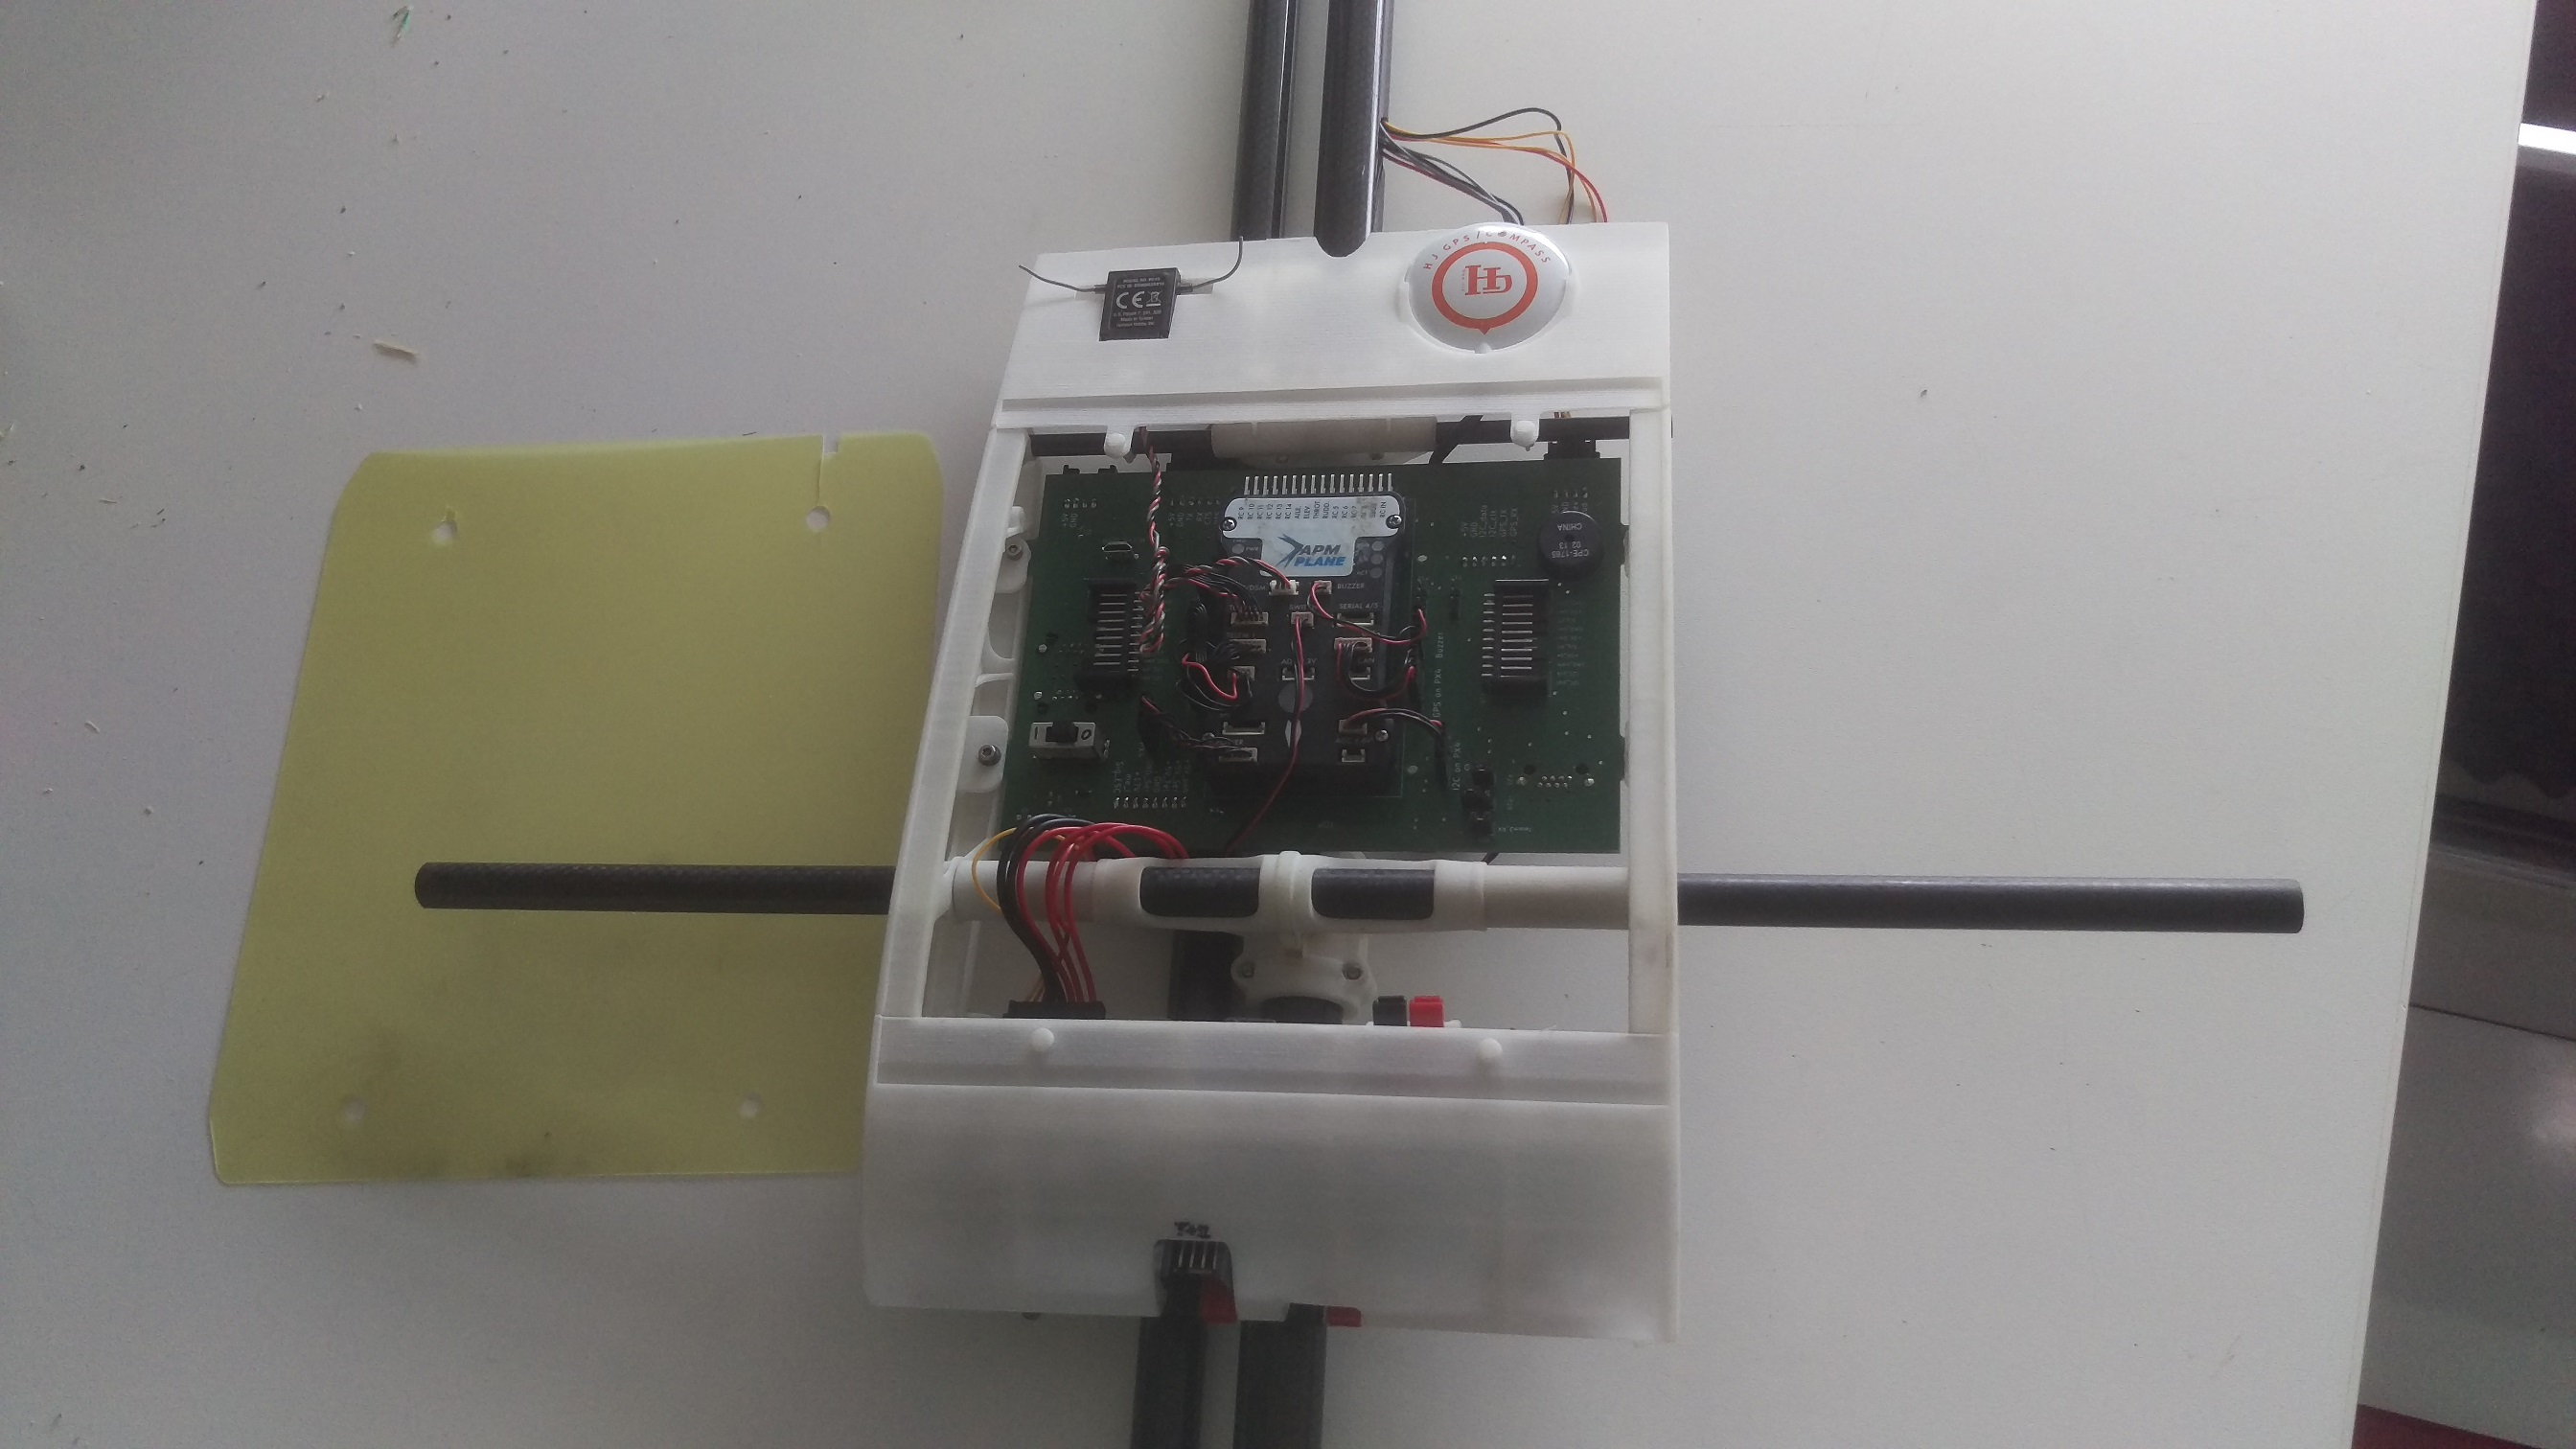
\includegraphics[width=0.9\textwidth]{bilder/Fotos/AUVSI_2016_Centerbox_Detail.jpg} 
\caption{In der WingCenterBox eingebaute Autopilotenplatine} 
\label{fig:In der WingCenterBox eingebaute Autopilotenplatine}
\end{figure}

\cleardoublepage

%\chapter{(optional) Fortschreitende Platinenentwicklung}\label{cha:Platinenentwicklung}

\section{Leistungsplatine}

\subsection{Schaltplan}

\subsection{Platinenlayout}

\section{Autopilotenplatine}

\subsection{Schaltplan}

\subsection{Platinenlayout}

\section{Platinenzusammenbau}

\cleardoublepage

\chapter{Erprobung im Labor}\label{cha:Erprobung im Labor}

Nach den anfänglichen Erfahrungen mit Ausfällen von Elektronik und Mechanik bei den ersten Generationen des Flugzeugs, werden alle Komponenten vor dem Einbau einzeln und nach der Montage als System im Labor getestet.
So können der Schadensumfang im Fehlerfall minimiert werden und die Emulation einzelner Betriebsszenarien ermöglicht eine einfache Eingrenzung möglicher Fehlerquellen.
In der Regel werden Szenarien wie die Maximalleistungsaufnahme beim Start und Steigflug sowie das Langzeitverhalten im Reiseflugzustand nachgestellt. Dabei werden relevante Parameter wie Temperatur der Bauteile gemessen und mit den Erwartungen verglichen.

\section{Einzeltests von Baugruppen}

Vor dem Einbau in das Gesamtsystem werden sowohl die einzelnen Platinen als auch ihre Modul Platinen einzeln Durchgetestet.
Dazu wird für die Leistungssysteme ein Labornetzteil als Quelle verwendet welches 0 - 45 V und 0 - 50 A zur Verfügung stellen kann.
Der Theoretische Nutzbereich des 4 Zelligen Akkusystems von 4,20 V bis 3,00 V je Zelle \footnote{\cite[Seite~1.12f.]{Reddy2010}} stellt einen Operationsbreichen von 16,8 V bis 12,0 V bereit. Deshalb wird für die meisten Tests eine Mittlere Spannung von 14,5 V gewählt. Der Strom wird auf etwa 30 A begrenzt um mögliche Fehlerfolgen zu begrenzen.
Die als kritisch eingestuften Bauteile werden mit Thermoelementen vom Typ K beklebt. Außerdem wird eine FLIR Thermokamera mit einer auflösung von 320x240 Pixel fest Aufgestellt um die Globale Themperaturverteilung auf dem PCB zu beobachten.
Da die absolute Genauigkeit der Temperaturwerte der Wärmebildaufnahmen aufgrund des ungekühlten CCD zumeist nicht korrekt sind, werden diese mit Hilfe der genauen werte der K Elemente skaliert.
Die Temperatur ist in unserem Leistungsbereich die Primäre Schadensursache. 
Um eine Vergleichbare Kühlungssituation aller getesteten Bauteile zu realisieren werden diese in der Ebene in Ruhiger Luft vermessen und auf Referenz Grundplatinen Montiert.
Dies ermöglicht eine Konservative Einordnung des Betriebspunktes da im Flugbetrieb alle Elektronikkomponenten vom Fahrwind überspült werden und damit von einer Verbesserten Kühlung auzugehen ist.

\subsection{Ideale Diode}

Die Messungen an dem Aufbau des Moduls der Idealen Diode beschränken sich auf das Verhalten als Leistungsbauteil. 
In Anlehnung an die Referenz Testaufbauten welche von Texas Instruments, Vishay Semiconductors und Toshiba Power Electronics für einzelne Mosfets in den zugehörigen Datenblättern verwendet werden ist auch die Adapterplatine für alle Idealen Dioden gestaltet.
Die Platine misst 1x1 Zoll mit 35 um Kupferstärke und regulärem Lötstopplack. Die ein und Ausgänge sind über Powerpol 55A Steckverbinder Realisiert. SMD Montierte Ösen ermöglichen den Abgriff der Differenzspannung über das gesamte Ideale Dioden Modul. In Einzelfällen wird zum Vergleich der Spannungsabfall über den reinen Mosfet Manuell zum Vergleich gemessen.

Die vegleichende Messung der beiden Generationen und verschiedener Mosfet Bestückungen zeigt die unterschiedlichen Equivalenten Wiederstände über den durchgeleiteten Strom.
Diese ist unmittelbar nach den Ohmschen Gesetzen für die örtliche Verlustleistung und damit für die Erwärmung der Baugruppe verantwortlich.

\begin{figure}[H]
\centering
\includegraphics[width=0.9\textwidth]{graphen/Wiederstand-Strom-Ideale_Diode_ver00} 
\caption{Wiederstandsverlauf} 
\label{fig:Wiederstandsverlauf}
\end{figure}


Wie aus der Grafik ersichtlich wird ist, wie erwartet der Mosfet als zentrales Schaltelement für quasi den Gesamten Wiederstand verantwortlich.
Eine Modifikation der Ersten Diodengeneration mit dem Austausch des Mosfet TPN2R304PL mit einem Nennwiederstand von 1,8\,$m\Omega$ \cite{TPN2R304PL} durch den Mosfet FDMC012N03 mit einem Nennwiederstand von 1,36\,m$\Omega$ \cite{FDMC012N03} reduziert den Equivalenten Wiederstand bei einem üblichen Akkustrom 10 A im Dauerbetrieb von 3,5\,$m\Omega$  auf 3,2\,$m\Omega$.
Demgegenüber stellt die zweite Generation eine deutliche Wiederstandserspranis dar.
Erreicht wir diese durch Ihre optimierte Wärmeableitung mit Neuanordnung der Bauteile und Verkleinerung des PCB sowie der nochmals veränderten Wahl des Mosfets auf TPHR6503PL.

Der höchste Dauerstrom liegt bei der unmodifizierten Generation eins bei 20\,A und bei der Generation 2 bei 30\,A. 
Generell wird der höchste Dauerstrom über die Baugruppe durch einen kleinstmöglichen Innenwiederstand des Verwendeten Mosfets und die Kupferfläche begrenzt auf welcher das Modul montiert ist um wärme Abstrahlen zu können. Das Modul PCB selbst hat aufgrund seiner geringen Größe eine vernachlässigbar kleine Kühlleistung.

Die Grafik zeigt zum Vergleich auch das Modul ohne Adapterplatine.

\subsection{5 Volt Servoversorgung}

Um die Eignung der zugekauften 5 V Spannungswandler zu evaluieren wurde exemplarisch ein Wandler mit einem Servo Impulsmäßig belastet.
Dabei wurde das Dc-Dc Modul mit 14,5 V versorgt und an den auf 5,0 V eingestellten Ausgang ein Servo Angeschlossen. Der Servo wurde von einem Servo Testgerät mit Steuersignalen versorgt welche ihn im Wechsel zu den jeweiligen Extrempositionen seines Verfahrbereichs dirigieren. 
An den 5,0 V Ausgang des Wandlers und das in den Servo laufende PWM Signal wurde ein  Digitaloszilloskop angeschlossen. Damit  wurde der Einbruch der 5 V Spannung, unter der Impulsartigen Strombelastung, des im Umkehrpunkt Beschleunigenden Servos beobachtet.
Damit sollte beurteilt werden ob der durch die Regelgeschwindigkeit und die Begrenzte Ausgangskapazität des Wandlers unvermeidbare kurzzeitige Einbruch im Millisekundenbereich in der Spannungsversorgung der Servos kritische Zustände verursacht.
Es könnte beispielsweise ein Zeitgleiches Ausschlagen mehrerer Servomotoren dazu führen das die Spannung so weit absinkt das keiner der Motoren noch funktionsfähig ist, beziehungsweise die Verfahrgeschwindigkeit deutlich absinkt.

Die Messung ergab einen Kumulierten Einbruch der Spannung um unter 0,5 V. 
Damit kann das Verhalten in allen erwarteten Flugsituationen als unkritisch bewertet werden. Gegebenenfalls wird hier in Zukunft zur weiteren Absicherung des Verhaltens noch eine Stützung mit Elektrolythkondensatoren umgesetzt. 

\section{Evaluierung der Signalpfade}

Es sollten Fehler im Schaltplan und im Routing der Platine ausgeschlossen werden. Dafür erfolgte ein Test der korrekten Signalführung ohne Einsatz der Sensoren und der Pixhawk Autopiloten Hardware. Dazu wurden an die Aus- und Eingänge des Pixhawk und der Sensoren ein 1 khz 50 Prozent PWM Signal angelegt um mit dem Oszilloskop die jeweils vorgesehene Gegenstelle Überprüft.

Dabei konnten auf der Autopiloten Platine keine Fehler festgestellt werden.
Auch die Inbetriebnahme der Sensoren und des Autopiloten verlief Hardwareseitig problemlos.

\section{Überprüfung der Logikfunktionen der Leistungsplatine}

Um eine einwandfreie Funktion und damit den sicheren Betrieb der Leistungsplatine sicherzustellen wurden deren Schutz und Regelfunktionen einzeln getestet.
Es wurden zunächst von einem Paket, aufsteigend alle Permutationen an Spannungsquellen an die drei vorgesehenen Anschlüsse gekoppelt und die Korrekte Führung der Energie überprüft.
Es wurde die vorgesehene Statusindikation durch Leuchtdioden verschiedener Farben dokumentiert.
Die Reguläre Führung der Quellen, Blockierung der Flugakkus im Bodenbetrieb und die Anzeige der Energiepfade funktionierte korrekt.

\section{Testlauf der Leistungsplatine}

Anschließend wurde die Platine in den Eingangs beschriebenen Flugmodi im dauerlauf getestet.
Bei den Tests im Startleistungsbereich stieg der Strom dabei auf einen Wert an, der dazu führte das der Sicherungsschalter in Richtung Motorversorgung Abschaltete.
Dies führte zu einer Oszillation des zugehörigen Mosfets zwischen Sperr- und Leitzustand. Der in diesem Übergangsbereich hohe innenwiederstand und der damit verbundene hohe Leistungsabfall am Mosfet führte bereits nach kurzer Zeit zur dessen Zerstörung durch Überhitzung.
Alle weiteren Versuche dieses Verhalten durch Dämpfung der Abschaltzeitschwelle oder Verbesserung der Kühlung blieben erfolglos. Deshalb wurden Aufgrund der geringen verbleibenden Zeit bis zum Wettbewerb diese Schaltung ersatzlos entfernt und mit einer entsprechenden Drahtbrücke überbrückt.

\cleardoublepage

%\chapter{(optional) Einsatz in der Flugerprobung}\label{cha:Einsatz in der Flugerprobung}

\section{Auftretende Fehler}

\subsection{Überstrom im Motortestlauf}

\subsection{Überspannung der 5 Volt Schiene}

\section{Anpassung des Elektronikonzepts}

\section{Anpassung der Bedienvorgaben}

\section{Fazit der Flugerprobung}

\cleardoublepage

%\chapter{(optional) Einsatz auf dem Wettbewerb}\label{cha:Einsatz auf dem Wettbewerb}

\section{Präsentation und Vergleich mit den Wettbewerbern}

\section{Ergebnis der Flugaufgabe}

\section{Wettbewerbserfolg}



\cleardoublepage

\chapter{Weitere Entwicklungen}\label{cha:Weitere Entwicklungen}

Nachdem die Grundlegende Plattform für das Projekt zu Verfügung steht befinden sich eine Reihe weiterer Verbesserungen und Innovationen in Arbeit. Diese sollen sowohl das Elektroniksystem bezüglich Handhabung, Sicherheit und Leistung optimieren, als auch neue Aspekte welche bisher keine genaue Beachtung erfahren haben, mit angepassten technischen Lösungen versehen.


\section{Entwicklung weiterer Funktionen als Modul}

Das Konzept des fertig aufgebauten, erprobten und bevorrateten Moduls der Idealen Diode als auflösbaren klein PCB hat sich bewährt. Eine Reihe von Anwendungen auch außerhalb der Flugzeugelektronik haben die Zeitersparnisse bei der Entwicklung gezeigt und eine zuverlässige Funktion gewährleistet.
Deshalb sollen weitere Systemfunktionen als Modul realisiert werden.
Eine interessante Gruppe der Sensoren sind hier Beispielsweise die Analog Digital Wandler (ADC). Während die Implementierung des einzelnen ADC in Hardware und Software aufwendig ist, ermöglicht die Anbindung an den I2C Bus den Einsatz vieler gleicher Messplatinen Beispielsweise zur Überwachung der einzelnen Akkuspannungen.
Auch bisher nicht realisierte Konzepte wie die Rückführung der Realen Ruderwinkel über Encoder oder Hall Sensoren sind in der Kombination aus PCB Modul und CAN Bus realisierbar.

Insgesamt bietet sich das Modulkonzept bei allen Elektrischen Bauteilen an bei denen ein hoher Aufwand für Auslegung, Layout und Erprobung betrieben werden muss um eine zuverlässige Funktion sicherzustellen.

\section{Betrachtung des CAN Bus}

Während in der manntragenden Luftfahrt der CAN Bus bereits seit langem zum Standard zur Übertragung von Sensordaten und auch Steuersignalen eingesetzt wird, wurde er bisher im Bereich kleiner UAV System kaum verwendet. Hauptgrund dafür stellt die strukturelle  Komplexität des vollständig Paket basierten Datenbusses dar, sowie die Softwareseitig aufwendige Adressierung und Verwaltung der einzelnen Teilnehmer.
Mit dem erscheinen des Pixhawk 2 wird der CAN Bus als regulärer Systembus geführt und seine Softwarepakte von der Offiziellen Entwicklergruppe gepflegt. Damit entfällt in Anbetracht der begrenzten Personal Ressourcen im Labor der bisher aufwendigste Aspekt der Nutzung dieses Systems. Eine Nutzung der hohen Stabilität bei geringer Leitungszahl und auch Flexibilität bei der Anzahl der Teilnehmer wird damit als Sensorbus möglich.
Entsprechend CAN Bus fähige Sensorplatinen sollen als Module konzeptioniert werden.

\section{Schnellwechsel-Akkusystem aus Rundzellen}

Neben den bisher eingesetzten Akku Packs aus Folienzellen stehen am Markt eine große Bandbreite und Rundzellen verschiedener Formate zur Verfügung. Als Industrielle Massenware stellen sie sich unter anderem als Preisgünstige Alternative dar.
Eine Analyse des Energie zu Gewicht Verhältnis ergab einen deutlich besseren Wert für die einzelnen Rundzellen gegenüber den Vorliegenden Folienzellen.Erste Prototypen eines Modularen Akkupakets aus 18650 Lithium Polymer Rundzellen der Firma LG lassen eine Verbesserung des kwh/kg Wertes um 15 bis 25 Prozent erwarten.
Außerdem soll der neue Packaufbau die Handhabung verbessern indem der Akkutausch ohne eine Demontage des Flügels möglich ist. Zur weiteren Vereinfachung soll auch das in den Röhrenförmige Paketaufbau integrierte Anschlussstecksystem beitragen.

Eine Erprobung der nötigen Verbindungstechniken und die Konstruktion eines Entsprechenden Gesamtpaketes findet derzeit statt.
Im weiteren Verlauf soll noch die genaue Integration in den Flügel und das gesamte Elektroniksystem gelöst werden.

\begin{figure}[H]
\centering
\adjincludegraphics[trim={0 15cm 0 15cm},width=0.9\textwidth,clip]{bilder/Fotos/Prototyp_18650er_Zellensystem.jpg}
\caption{Zweiter Prototyp der Rundzellenpakets} 
\label{fig:Zweiter Prototyp der Rundzellenpakets}
\end{figure}


\section{Migration auf die nächste Pixhawk Generation}

Im Zuge des Wachstums des Pixhawk Projekts wurde eine neue Generation von Hardware für den ArduPilot Autopiloten entworfen und in den Software Branch eingepflegt. Diese leistungsgesteigerte Version steht seit Anfang 2017 zu Verfügung.
Sie verfügt neben mehr Prozessorleistung und redundanten integrierten Sensoren über eine DF17 80 Pin Schnittstelle der Firma JST. Damit ist eine noch Platzsparendere Unterbringung des Pixhawk möglich und es werden weitere Kabelverbindungen eingespart.

Um diese Komponente in Zukunft im Flugsystem nutzen zu können, wird eine Entsprechende Platinenentwicklung und die Nötige Integration seit Sommer 2017 von Michael Simbürger durchgeführt\cite{Simburger}.

\begin{figure}[H]
\centering
\adjincludegraphics[trim={5cm 15cm 5cm 15cm},width=0.9\textwidth,clip]{bilder/Fotos/Pixhawk2_Autopilot_PCB_2018_Simbuerger.jpg}
\caption{Neue Pixhawk 2 Autopilotenplatine für 2018 von Michael Simbürger} 
\label{fig:Neue Pixhawk 2 Autopilotenplatine für 2018 von Michael Simbürger}
\end{figure}

%\section{Erfahrungen aus dem Feldeinsatz}

%\section{Anpassung der Anforderungen an die Elektronik}

%\section{Detailverbesserungen an den Komponenten}

%\section{Technischer Ausblick}

\cleardoublepage

\chapter{Fazit und Ausblick}\label{cha:Fazit und Ausblick}

In den letzten Jahren hat sich die Elektronik des Automatischen Flugsystems des Labor für Systemtechnik sich seinen vielfältigen Aufgaben angepasst.
Dabei hat sich sowohl die Augabenformulierung und das Konzept von ersten Versuchen nahe einem klassischen Modellflugzeug zu einem vollständigen System mit Platinenaufbau und zahlreichen Unteraufgaben gewandelt. Es ist ein vielfältiges Repertoire an erprobten und gereiften Elektronikbaugruppen entstanden welche sich in stetiger Optimierung befinden. Damit ist sowohl eine schnelle Anpassung der Gesamten Elektronik an neue Aufgaben und Dimensionierungen möglich.
Damit hat die Elektronik die vorausgegangene Entwicklung des mechanischen Aufbaus nachvollzogen, welche auch eine gezielte Verbesserung einzelner Funktionen bei begrenztem Arbeitsaufwand ermöglicht.
Ebenfalls ist mit den gewachsenen Erfahrungen mit dem Einsatz des Flugsystems im Zusammenspiel mit den Elektronischen Schutzmaßnahmen ein hohes Sicherheitsniveau für Bedienmannschaft und Flugzeug gewährleistet. Dies hat sich besonders im oft hektischen Wettbewerbseinsatz als wertvoll erwiesen.

Wie das Kapitel der weiteren Entwicklungen bereits aufzeigt entstehen auch Abseits der eigentlichen Schaltungsentwicklung neue Ansätze und Aspekte um Handhabung und Leistungsfähigkeit des Gesamtsystems zu steigern.

Somit wird das Elektronische Gesamtsystems des Automatischen Flugsystems des Labor für Systemtechnik auch in den kommenden Jahren konkurrenzfähig auf dem AUVSI Wettbewerb antreten können, als sich auch kurzfristig in Forschungseinsätzen bewähren.




\cleardoublepage

% Setze Numerierung wieder auf römisch zurück und setzte von oben fort
% Wert ist demnach der von 'roemisch'
\newpage
%\pagenumbering{Roman}
%\setcounter{page}{\value{roemisch}}

% Maxi Biblio-Management
\bibliography{literatur/bib}

% Zinz Biblio-Management
% %\printbibheading[title=Quellenverzeichnis]
% %\printbibliography %[heading=none]
% %\printbibliography[keyword=Literatur, heading=subbibliography, title={Literaturverzeichnis}]
% %\printbibliography[keyword=Quelle, heading=subbibliography, title={Quellenverzeichnis}]

%
% Abbildungsverzeichnis
%
\listoffigures

%
% Tabellenverzeichnis
%
\listoftables

\cleardoublepage


%\begin{comment}
% Appendix, falls vorhanden
\appendix
%\chapter{Anhang}

\begin{table}[H]
\centering
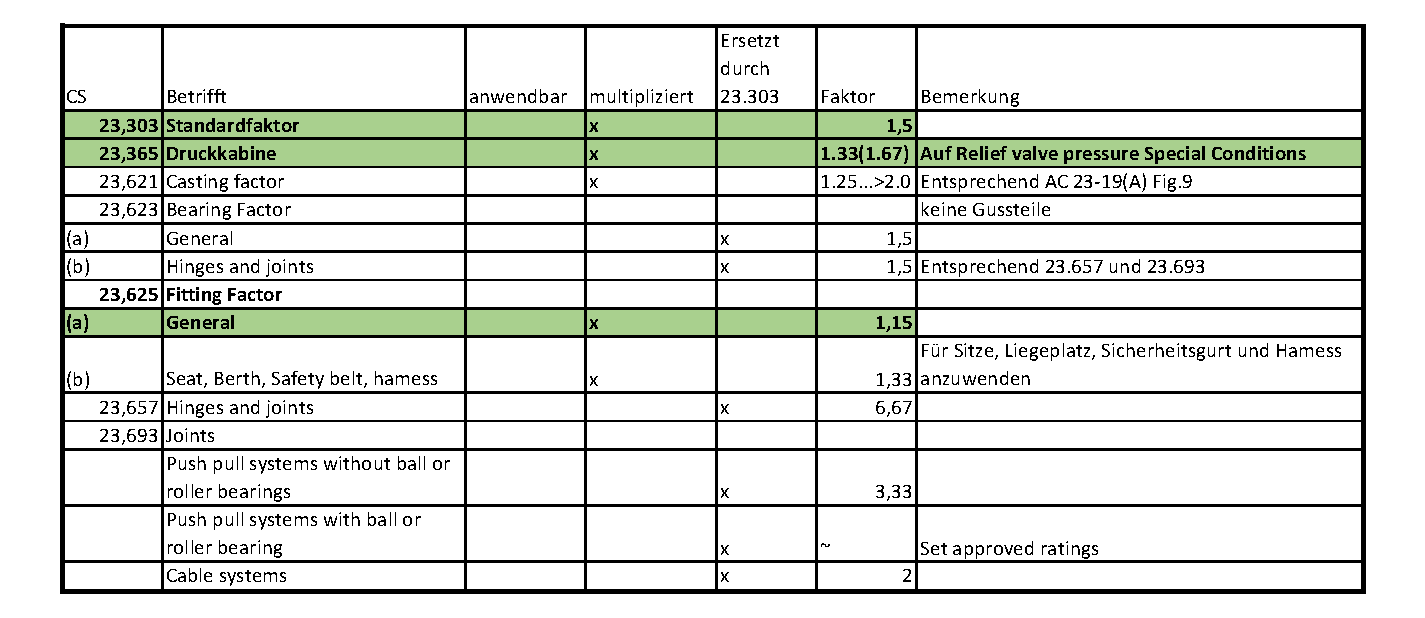
\includegraphics[width=0.9\textwidth]{bilder/Tabellen/Sicherheitsfaktoren.pdf}
\caption{Formblatt F021 - Nachweis der geforderten Sicherheit am Schnitt} 
\label{tab:Sicherheiten}
\end{table}

\clearpage

\begin{table}[H]
\centering
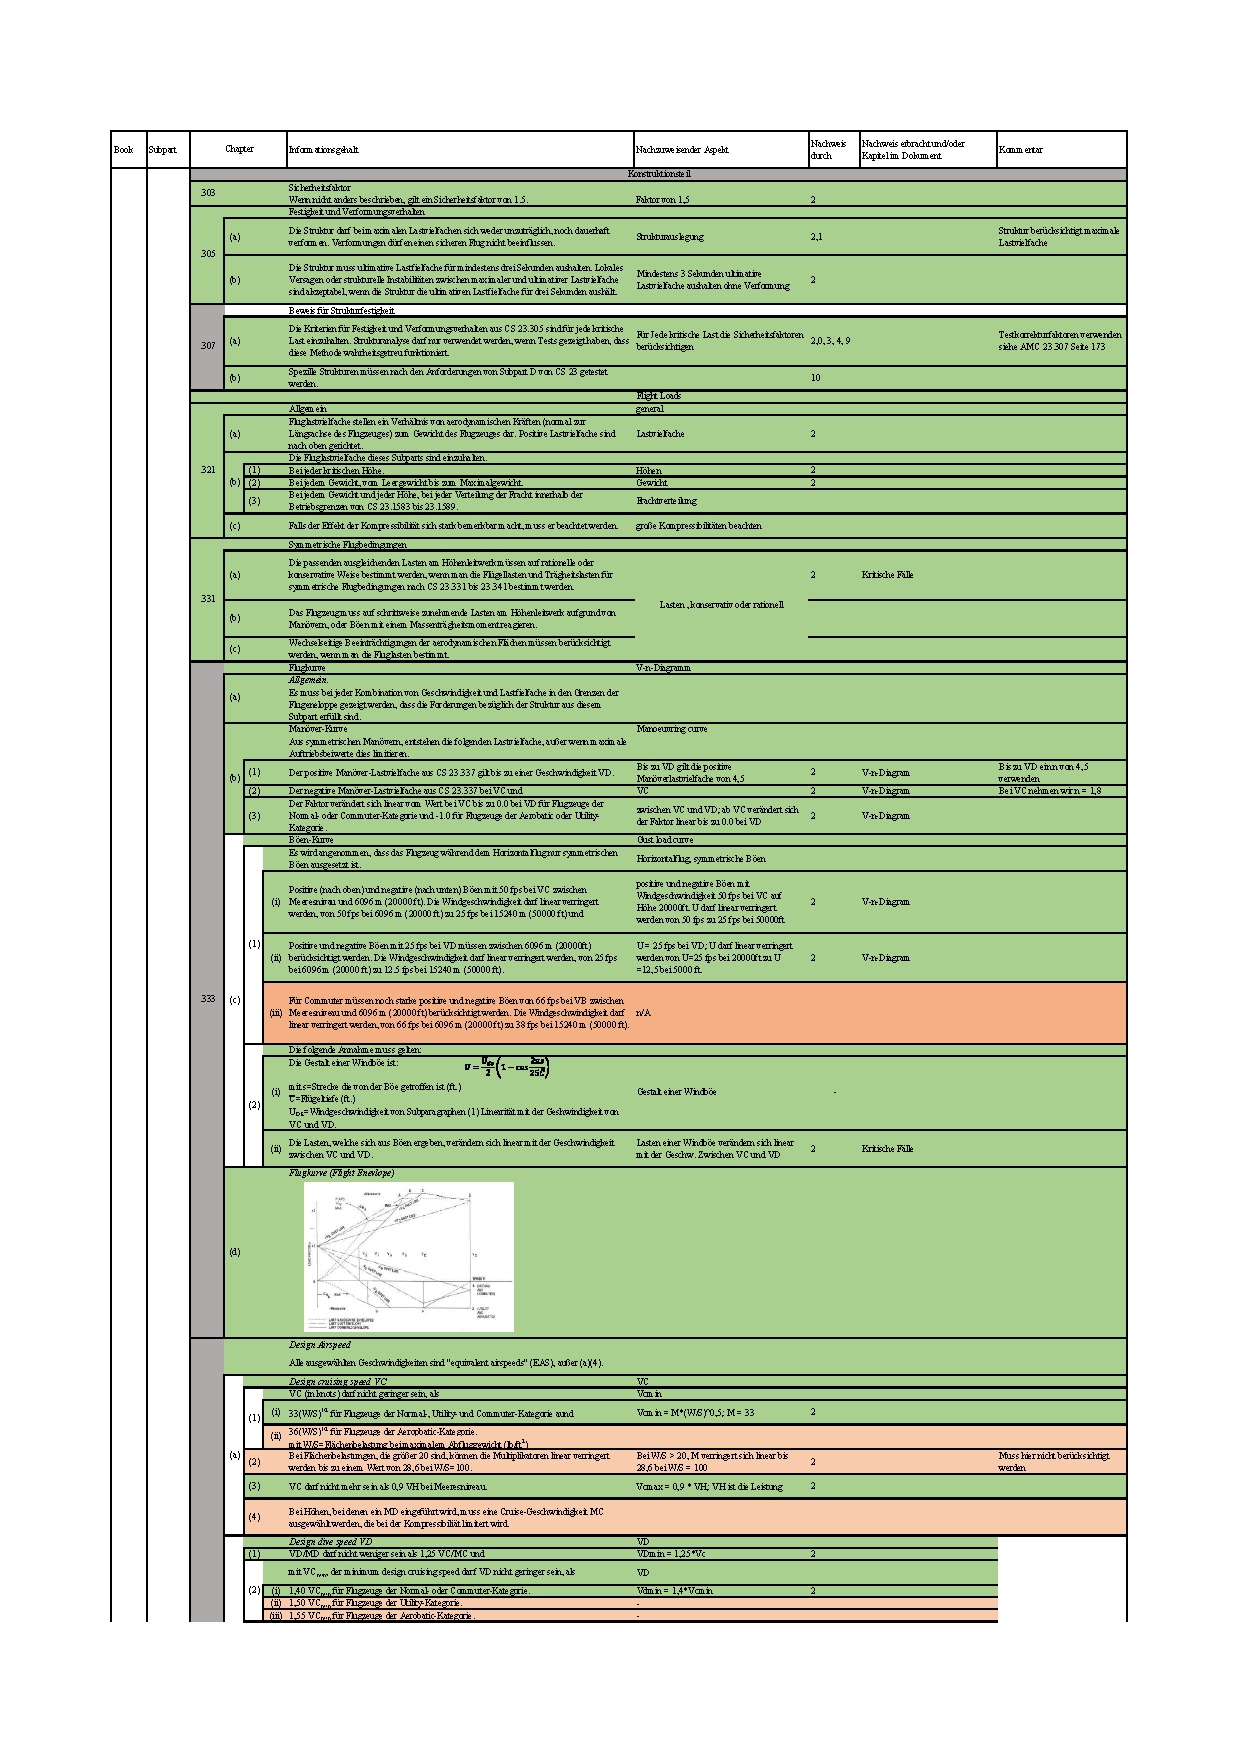
\includegraphics[width=0.9\textwidth]{bilder/Tabellen/MPP_Konstruktion_1.pdf}
\end{table}

\begin{table}[H]
\centering
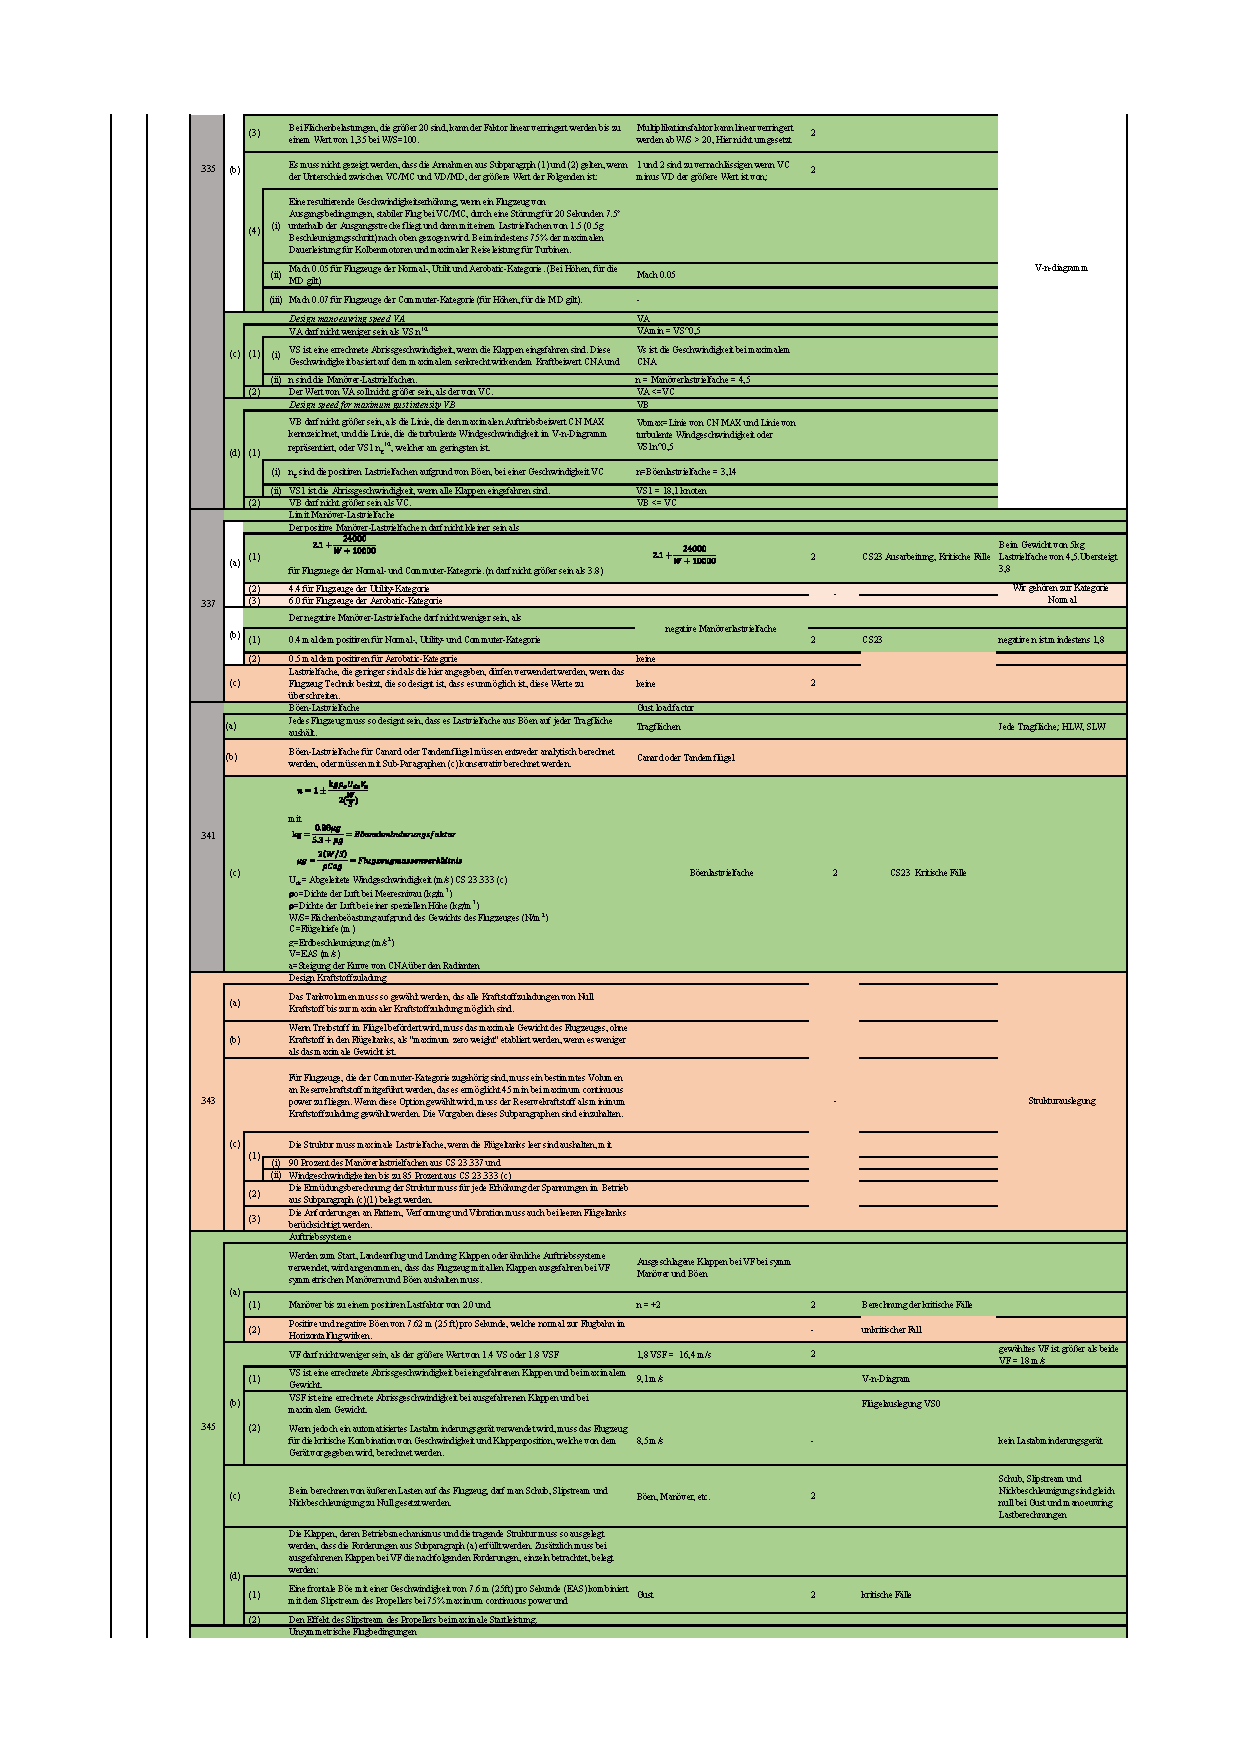
\includegraphics[width=0.9\textwidth]{bilder/Tabellen/MPP_Konstruktion_2.pdf}
\end{table}

\begin{table}[H]
\centering
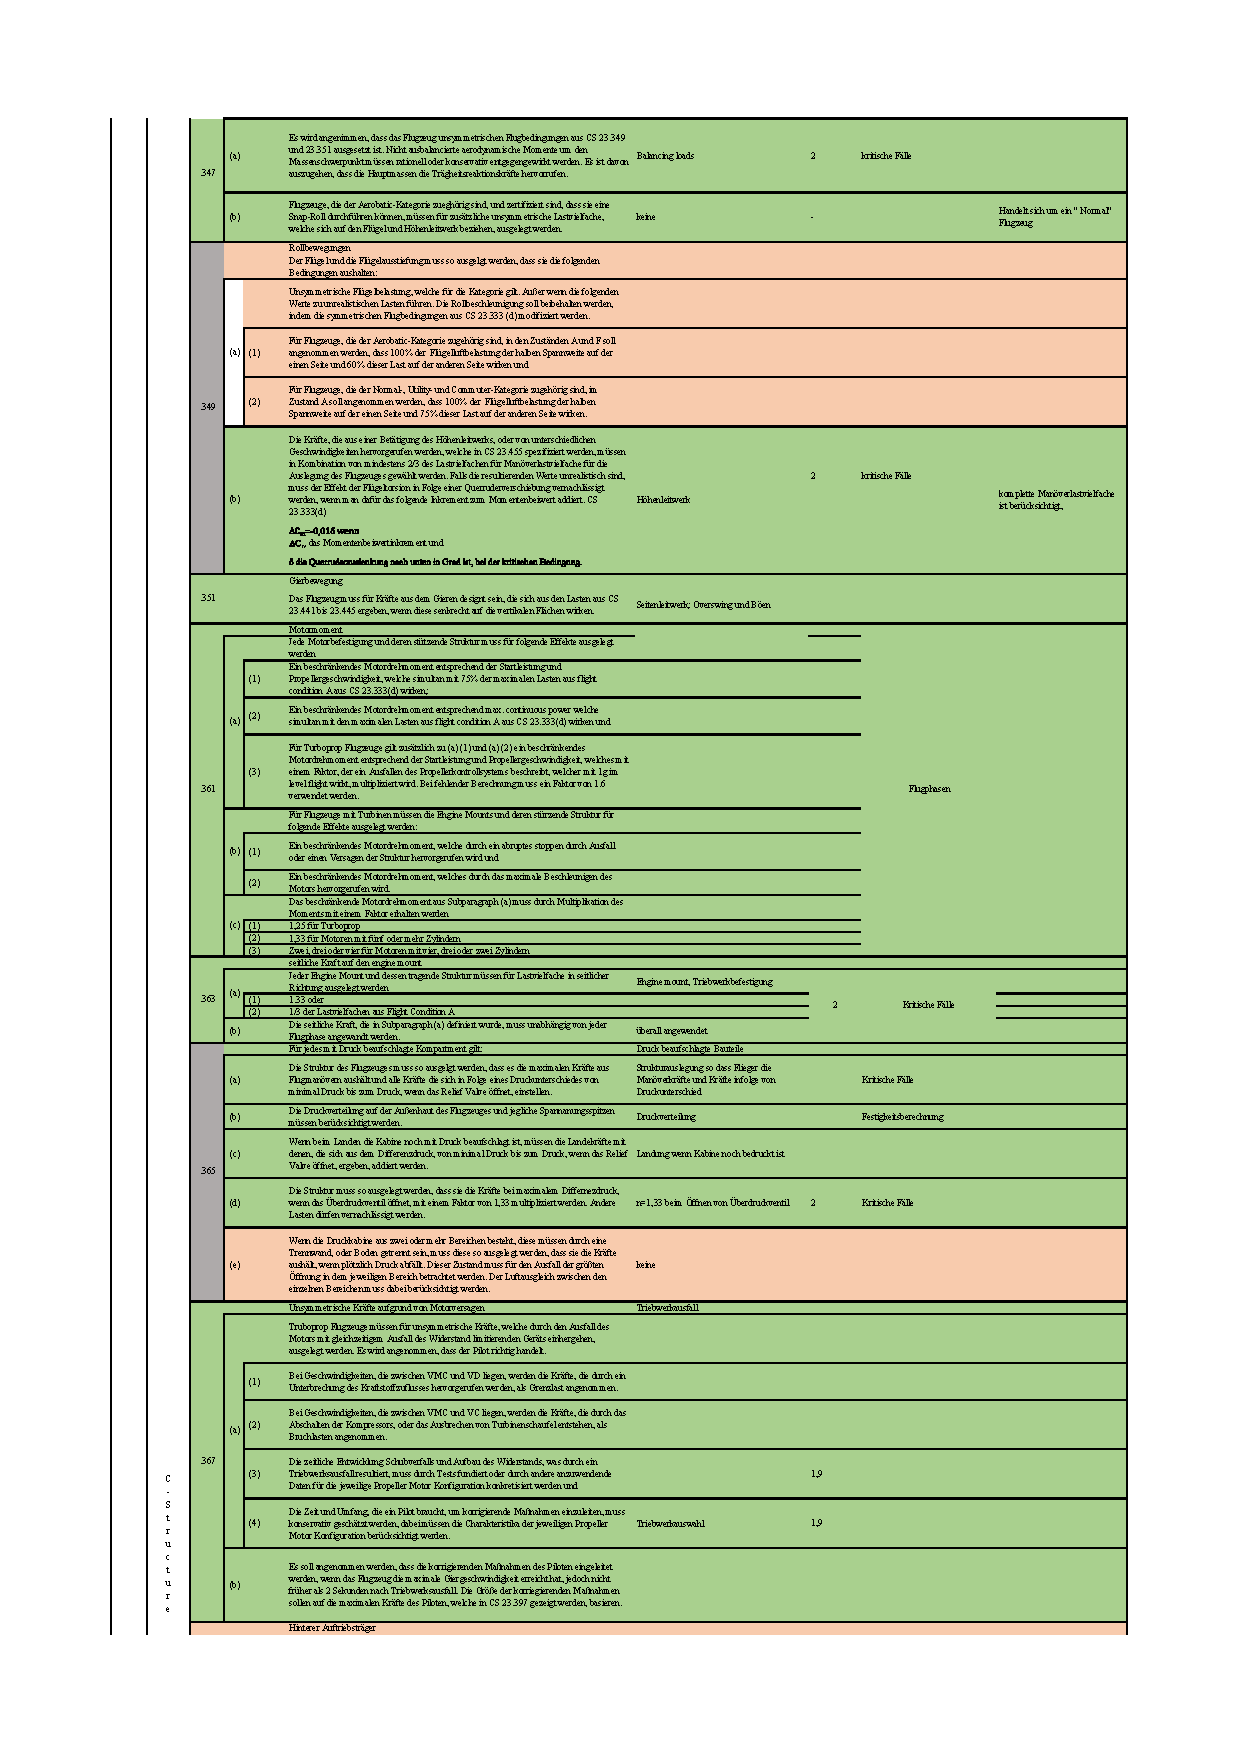
\includegraphics[width=0.9\textwidth]{bilder/Tabellen/MPP_Konstruktion_3.pdf}
\end{table}

\begin{table}[H]
\centering
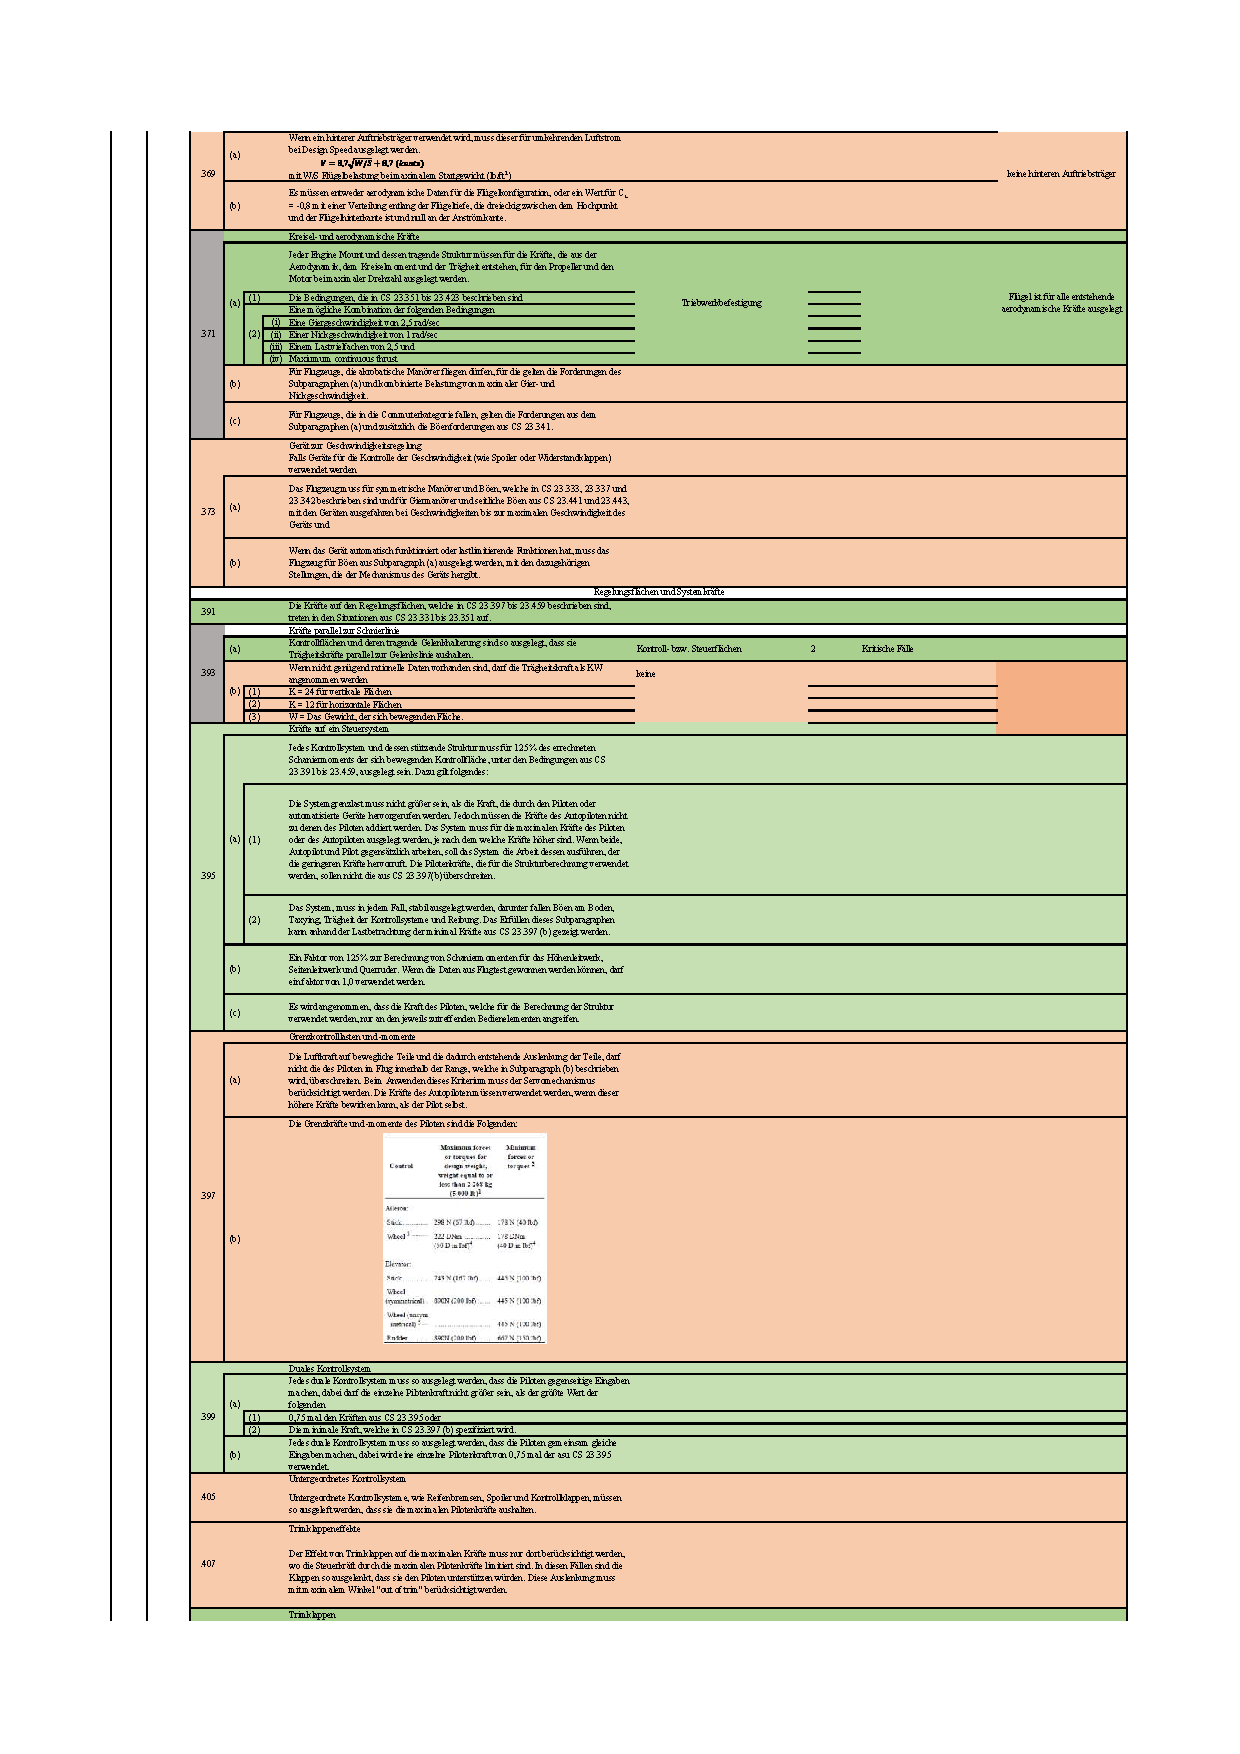
\includegraphics[width=0.9\textwidth]{bilder/Tabellen/MPP_Konstruktion_4.pdf}
\end{table}

\begin{table}[H]
\centering
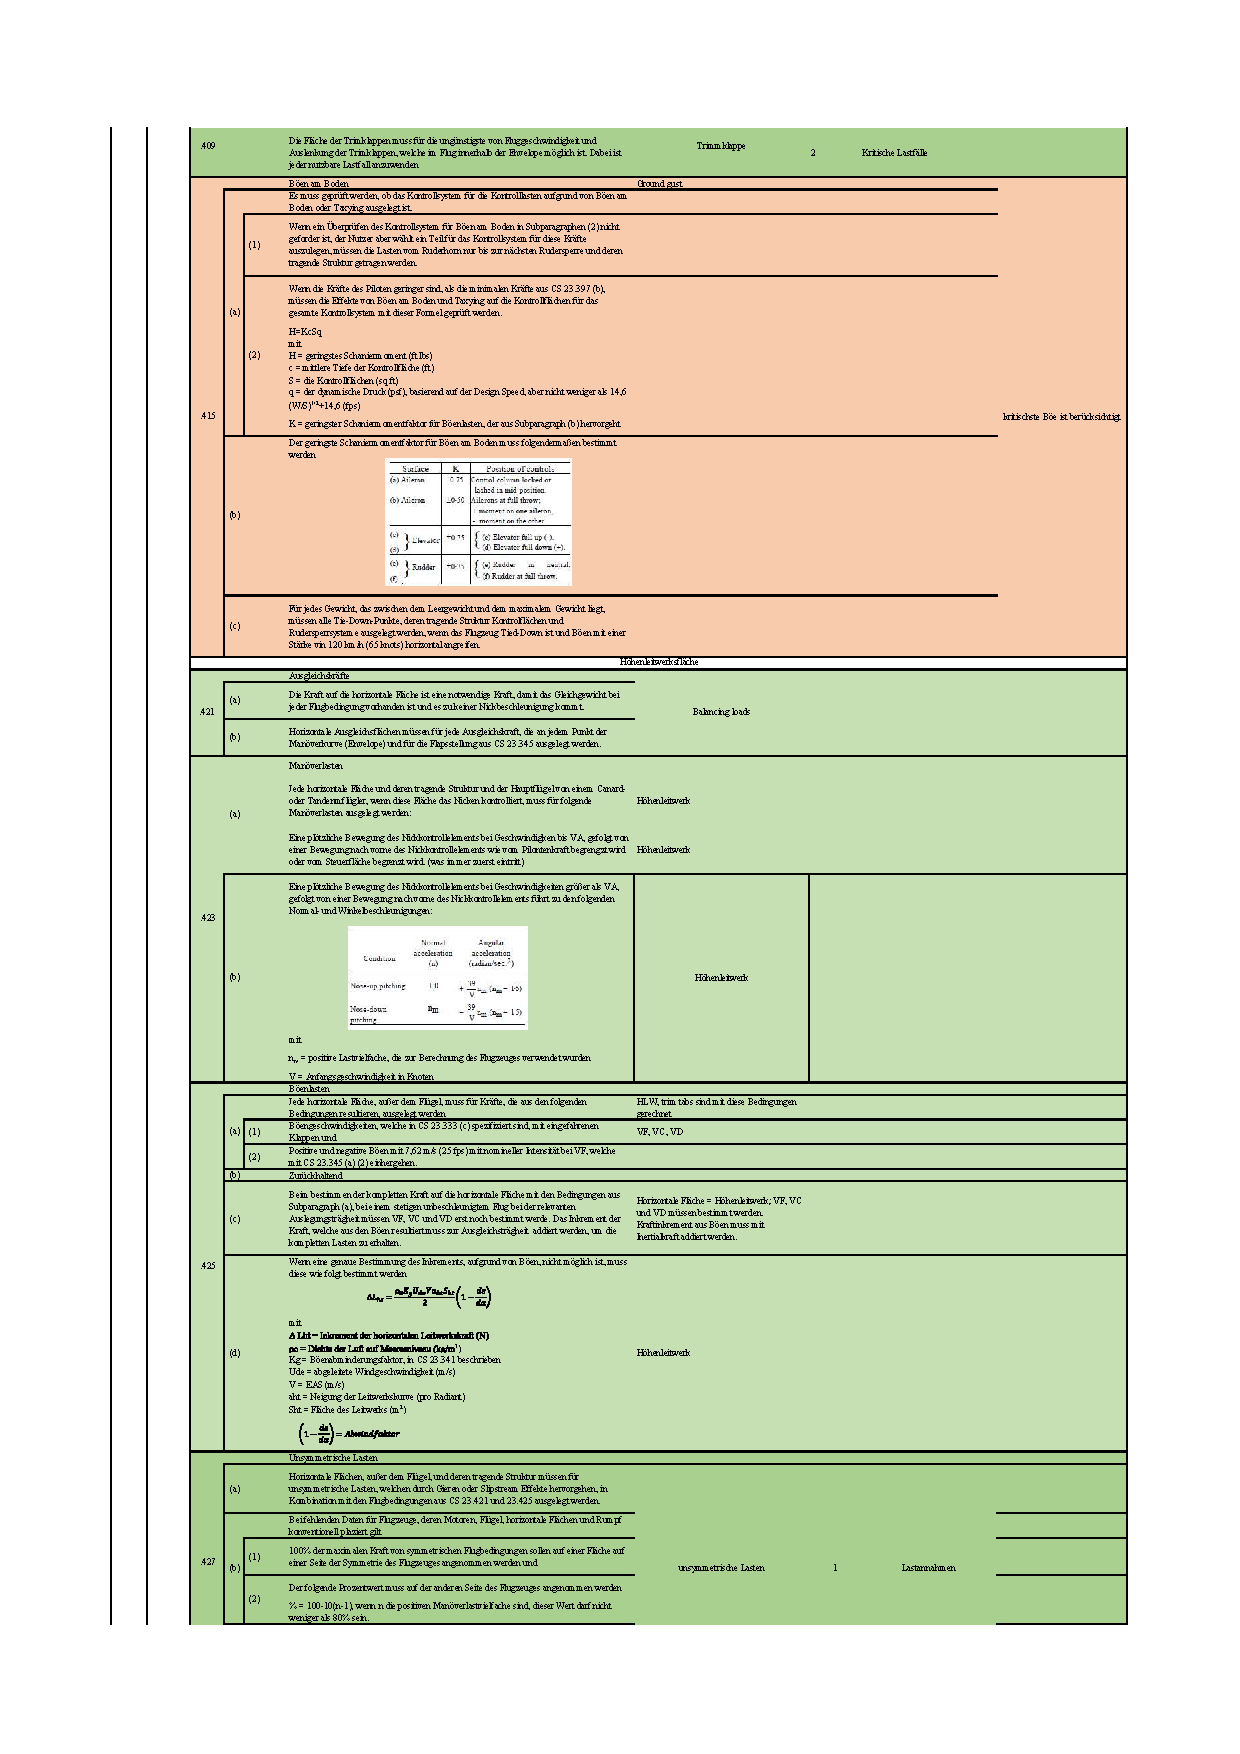
\includegraphics[width=0.9\textwidth]{bilder/Tabellen/MPP_Konstruktion_5.pdf}
\end{table}

\begin{table}[H]
\centering
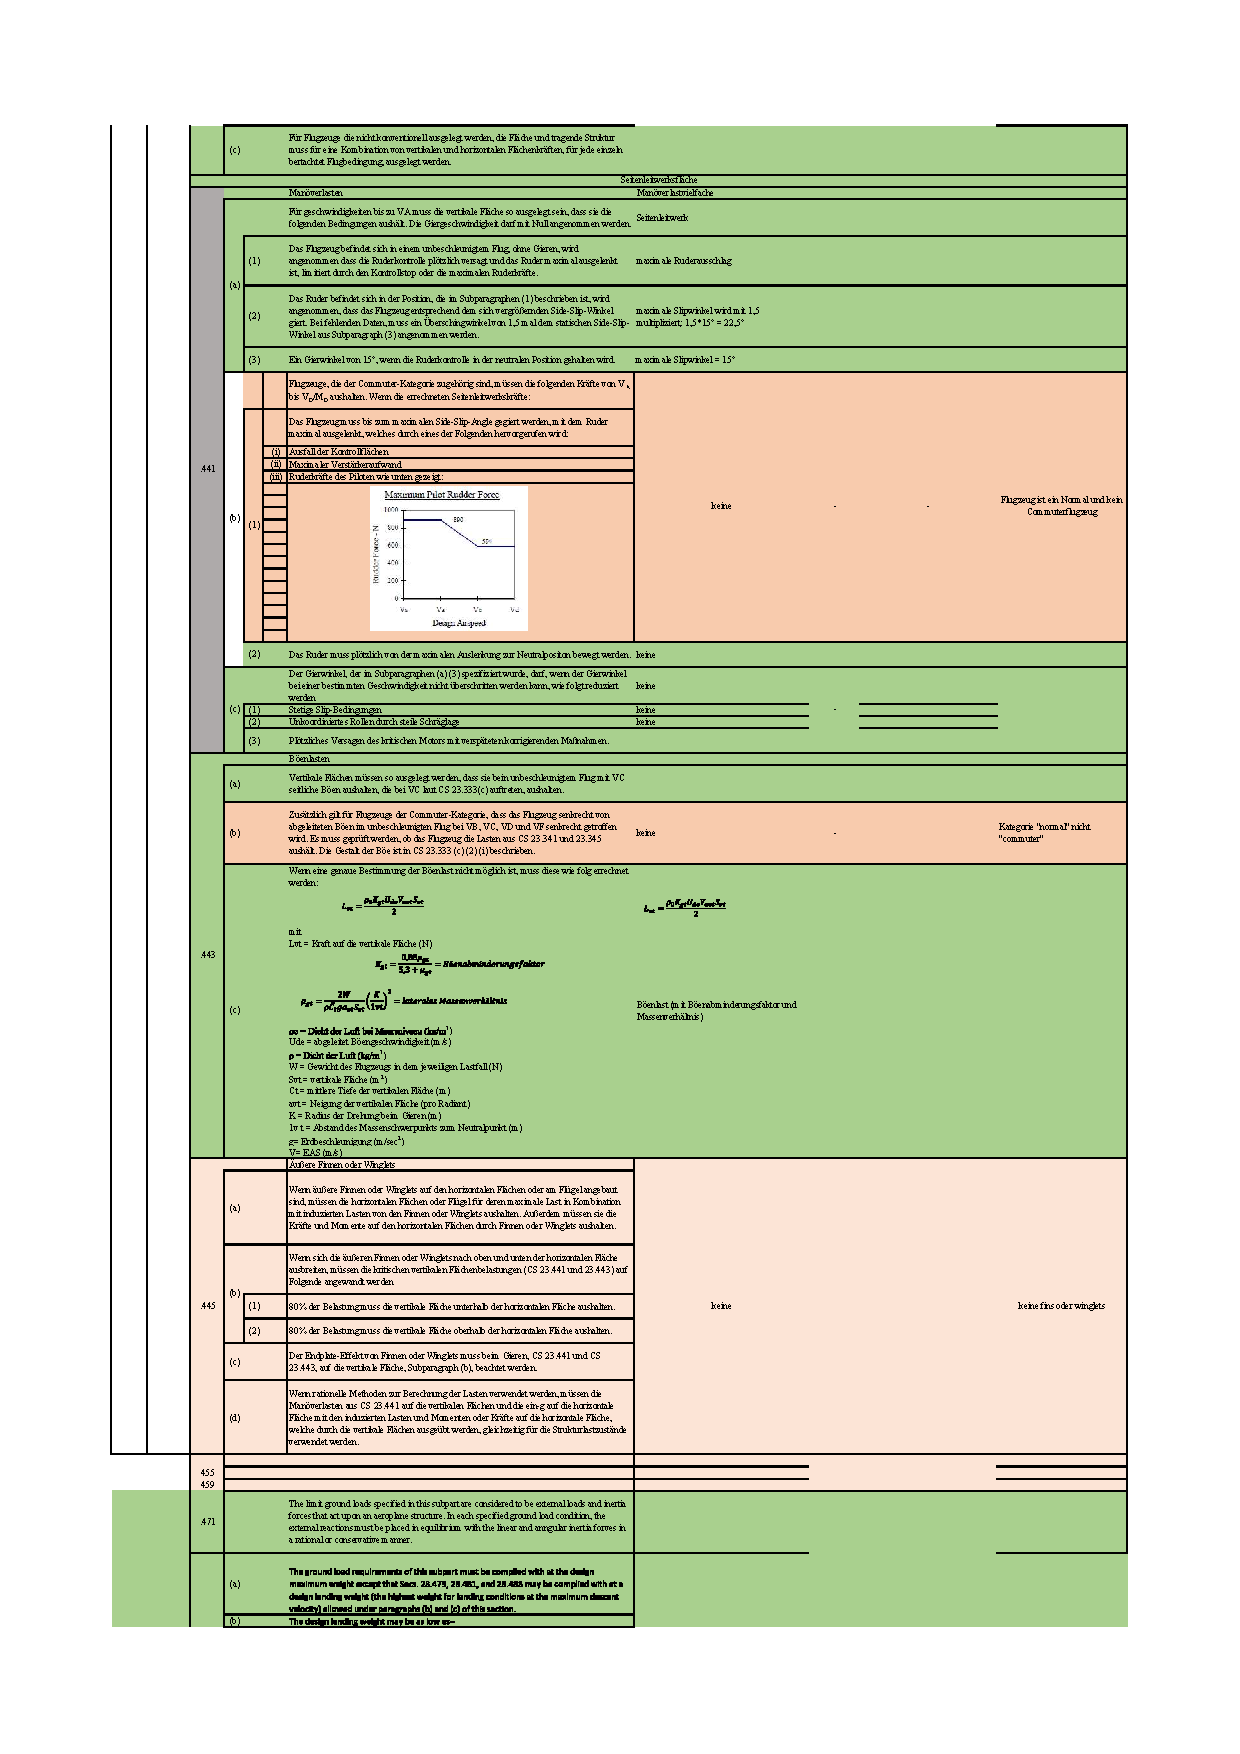
\includegraphics[width=0.9\textwidth]{bilder/Tabellen/MPP_Konstruktion_6.pdf}
\end{table}

\begin{table}[H]
\centering
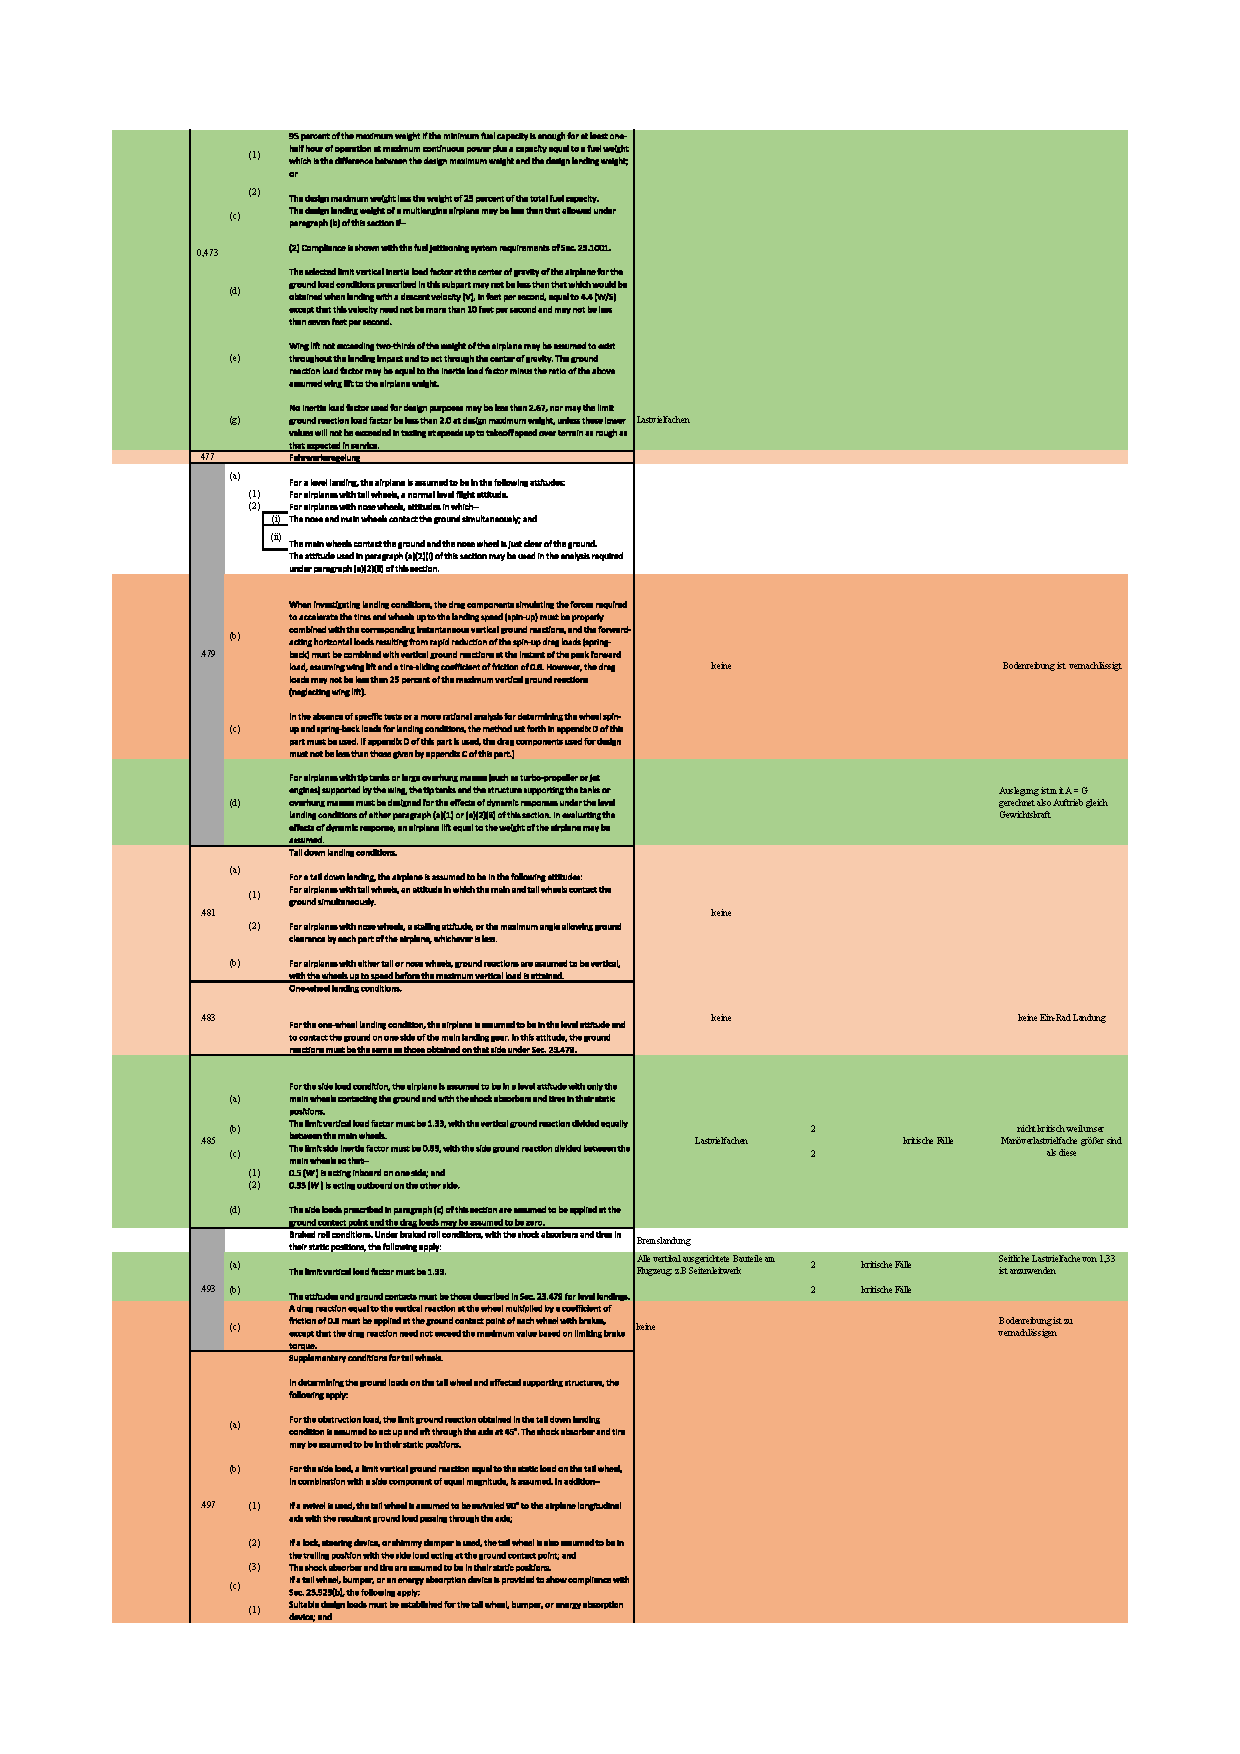
\includegraphics[width=0.9\textwidth]{bilder/Tabellen/MPP_Konstruktion_7.pdf}
\end{table}

\begin{table}[H]
\centering
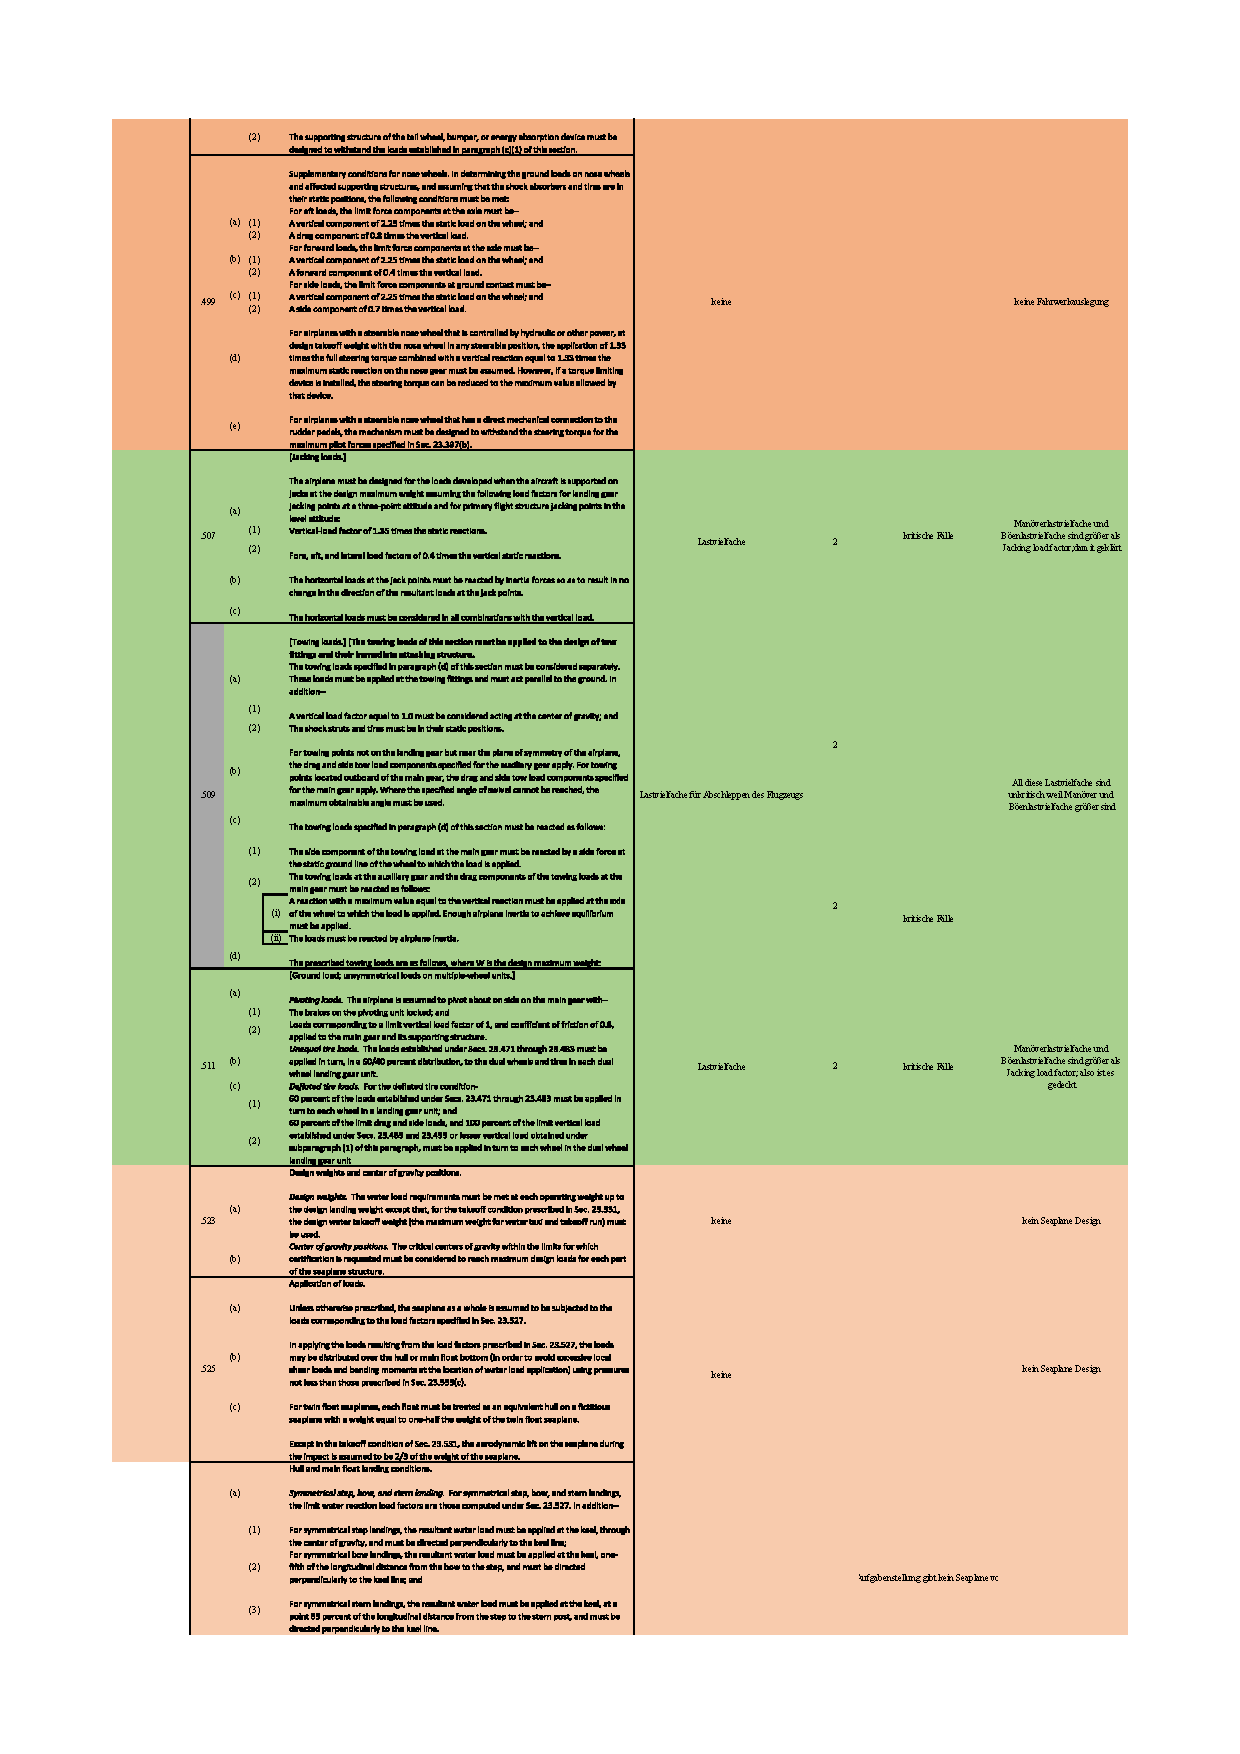
\includegraphics[width=0.9\textwidth]{bilder/Tabellen/MPP_Konstruktion_8.pdf}
\end{table}

\begin{table}[H]
\centering
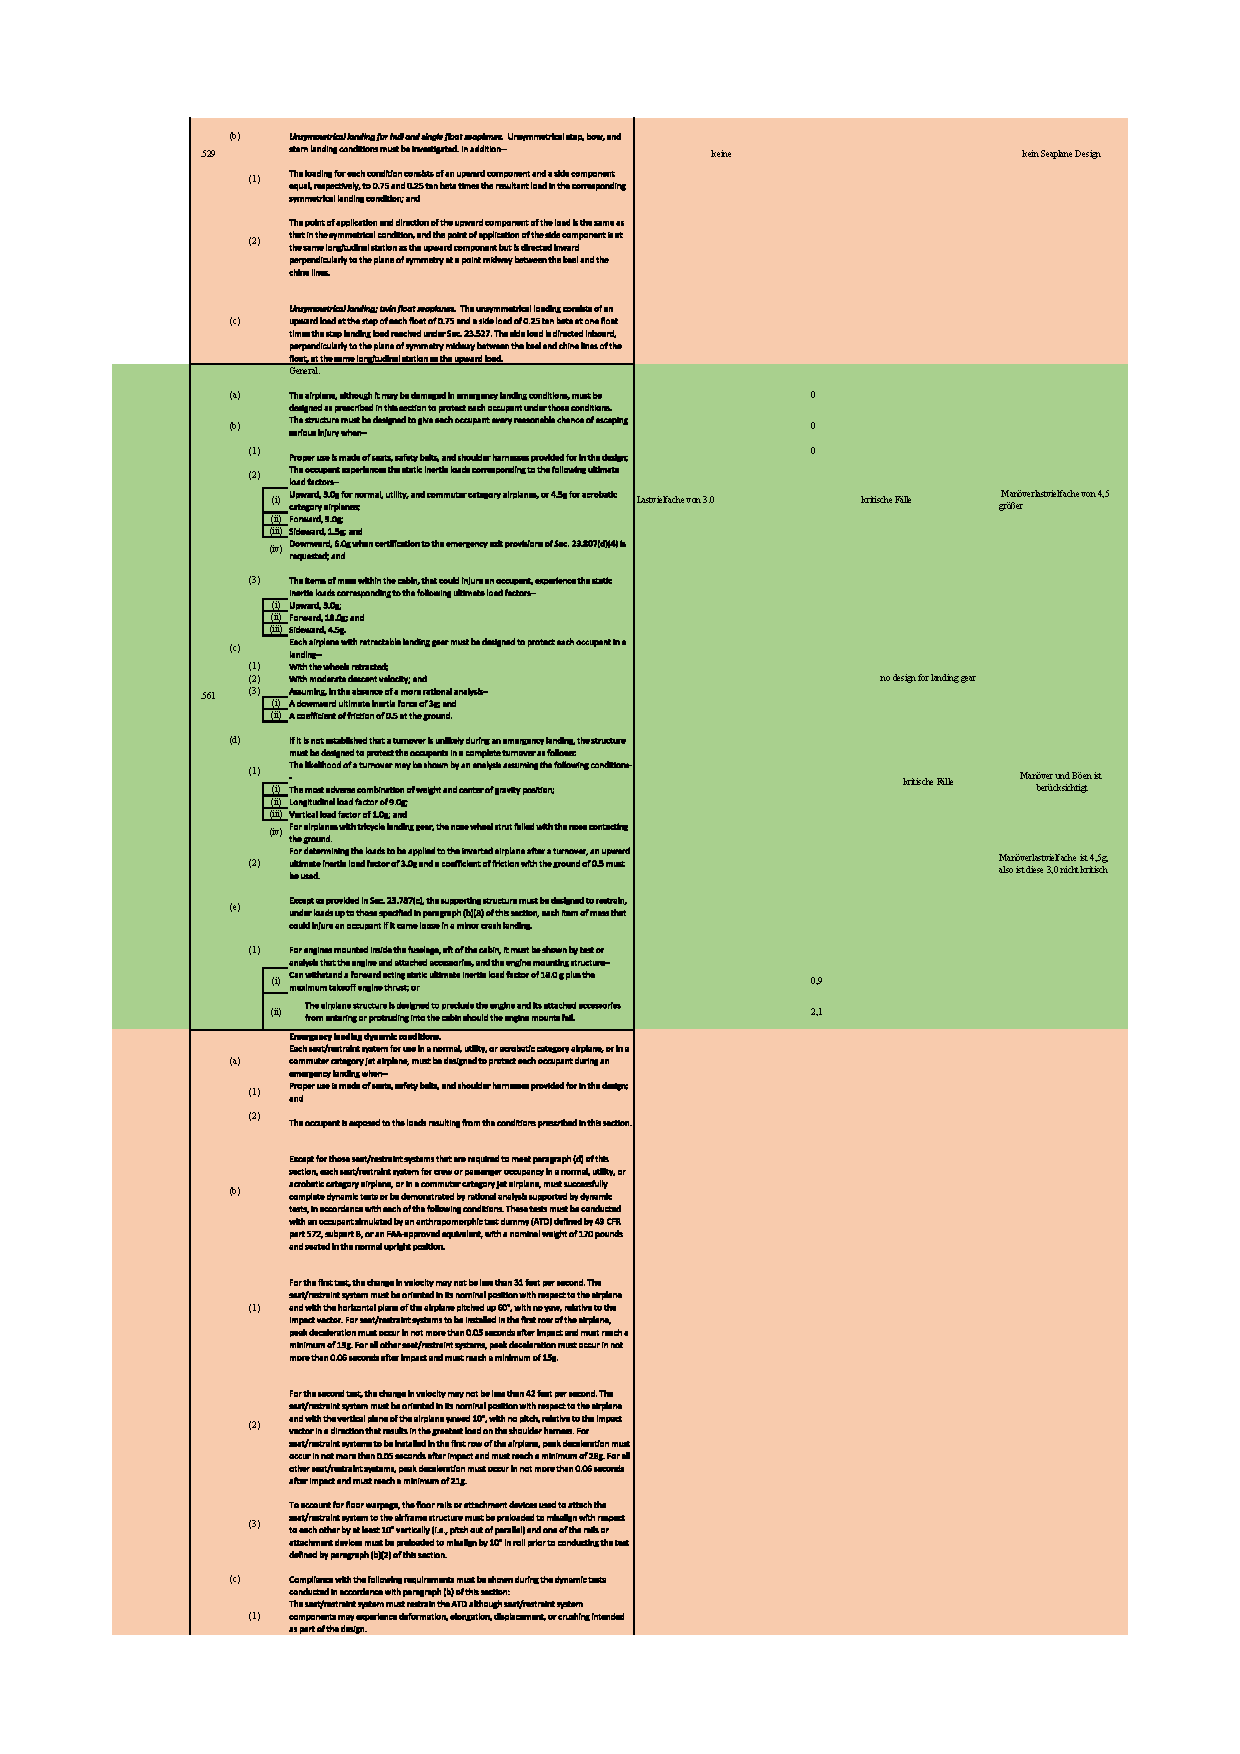
\includegraphics[width=0.9\textwidth]{bilder/Tabellen/MPP_Konstruktion_9.pdf}
\end{table}

\begin{table}[H]
\centering
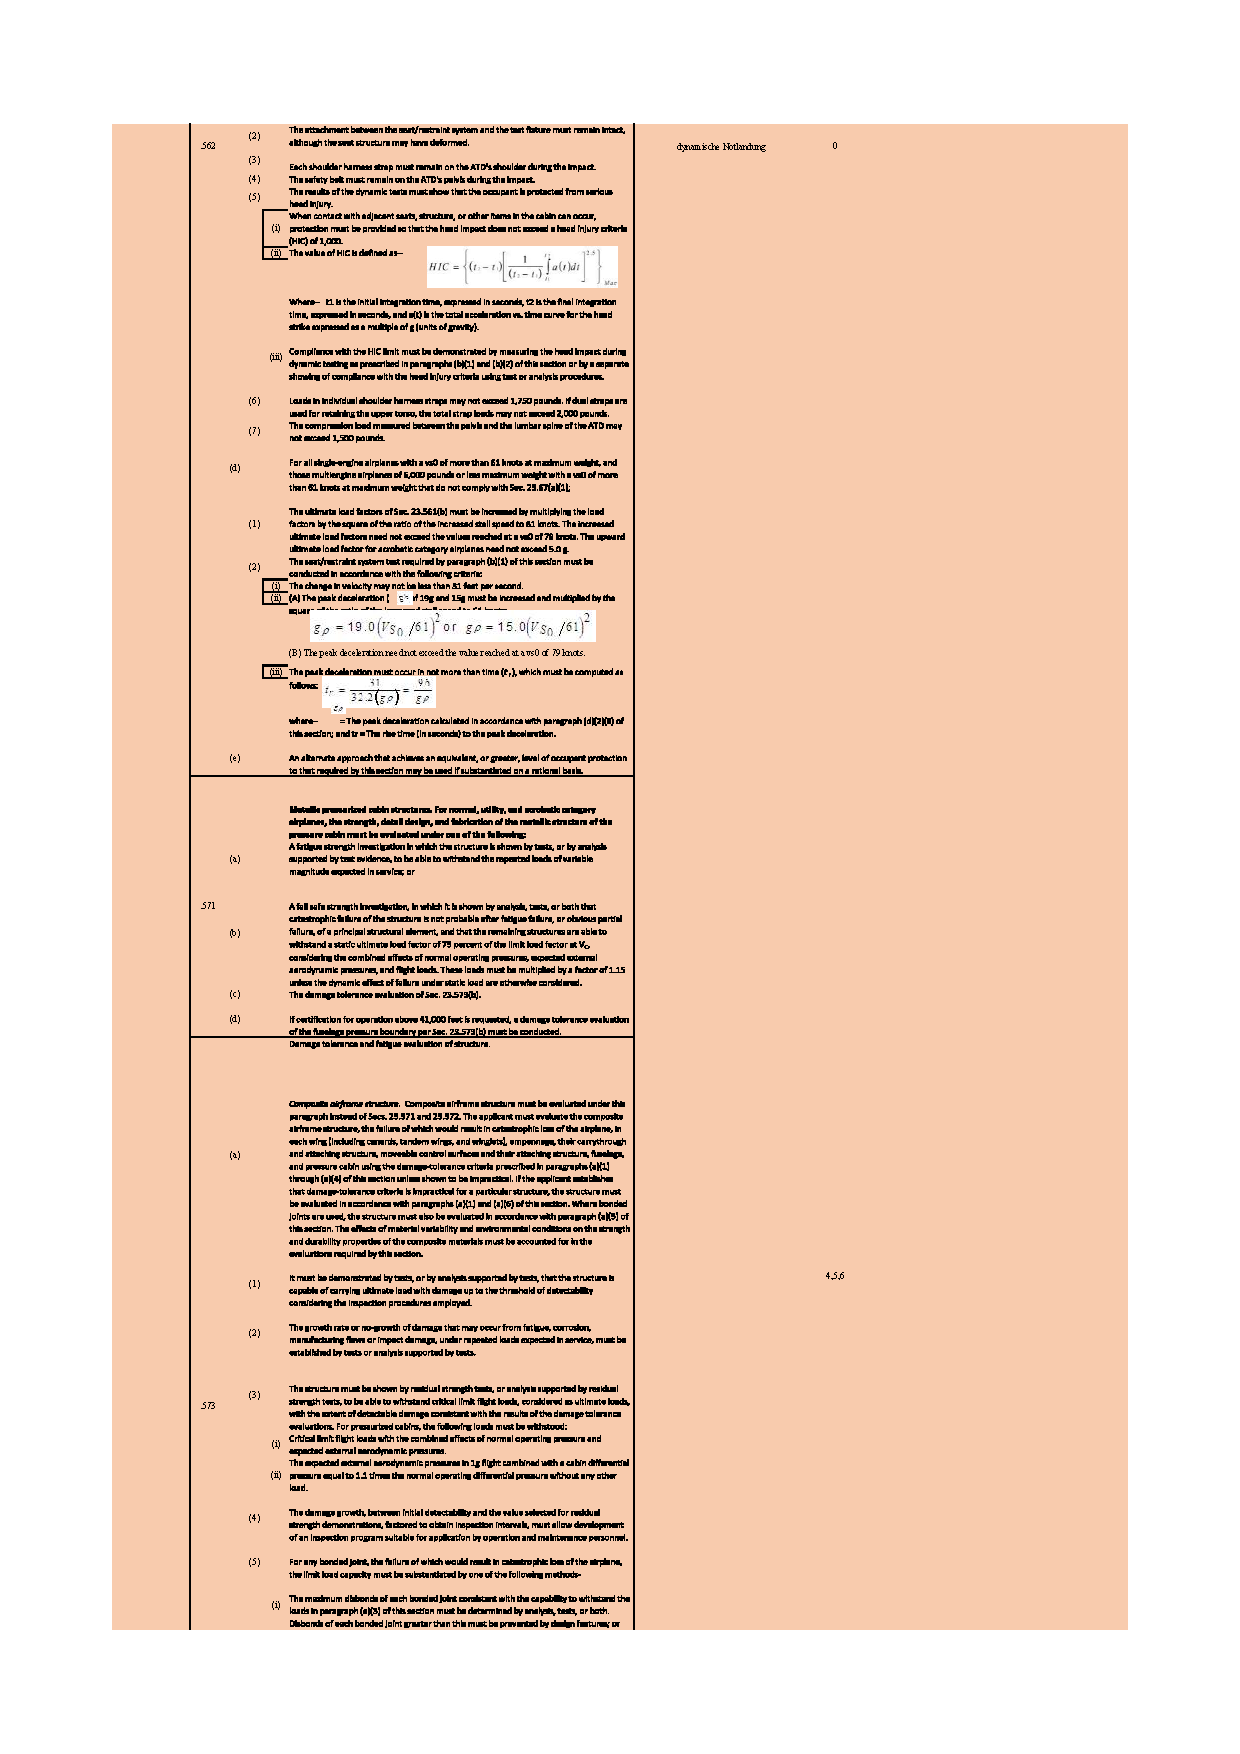
\includegraphics[width=0.9\textwidth]{bilder/Tabellen/MPP_Konstruktion_10.pdf}
\end{table}

\begin{table}[H]
\centering
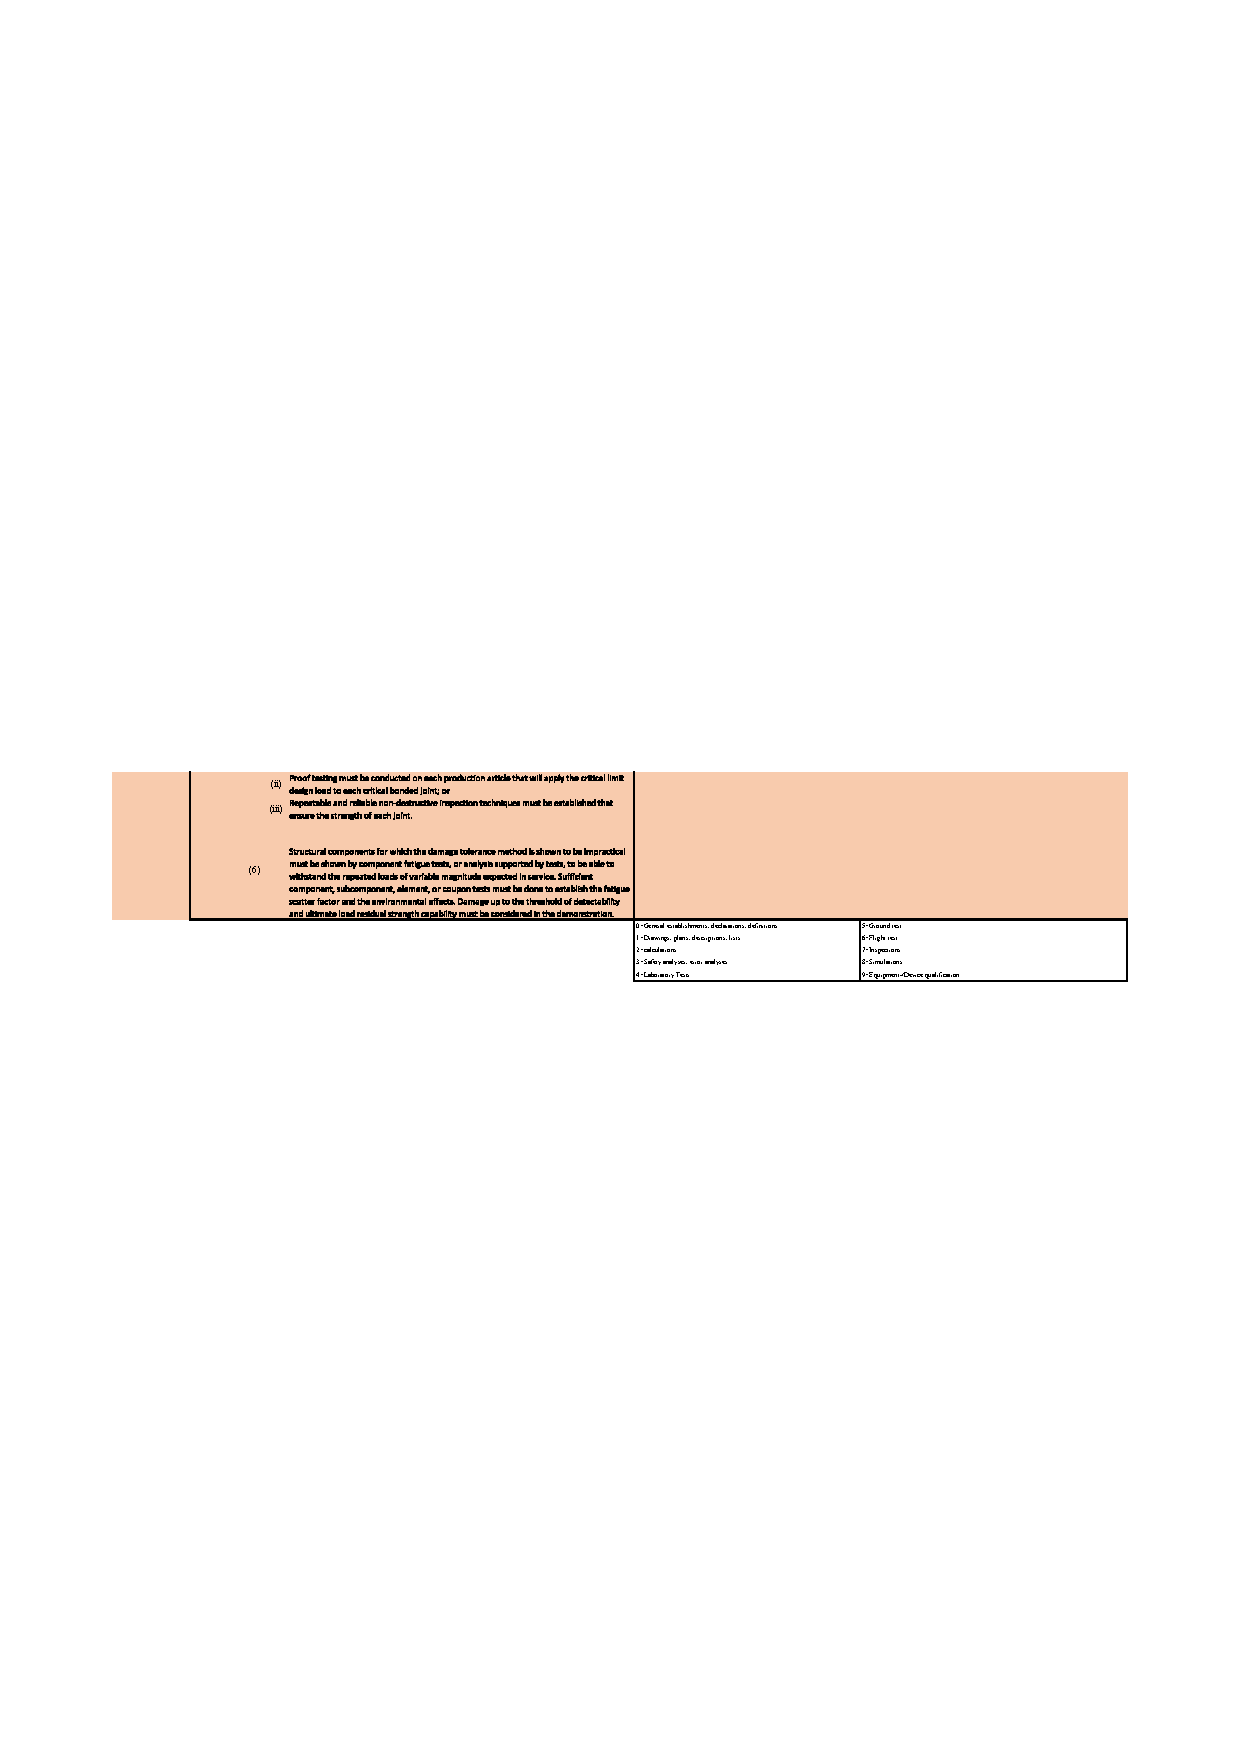
\includegraphics[width=0.9\textwidth]{bilder/Tabellen/MPP_Konstruktion_11.pdf}
\caption{Musterprüfplan} 
\label{tab:Musterprüfplan}
\end{table}

%\clearpage

\section{}\label{}



%\end{comment}


% Eidesstattliche Erklärung
%% Die eidesstattliche Erklärung mit Unterschrift
\chapter*{Erklärung der Urheberschaft}\addcontentsline{toc}{chapter}{Erklärung der Urheberschaft}

Ich erkläre hiermit an Eides statt, dass ich die vorliegende Arbeit
ohne Hilfe Dritter und ohne Benutzung anderer als der angegebenen
Hilfsmittel angefertigt habe; die aus fremden Quellen direkt oder
indirekt übernommenen Gedanken sind als solche kenntlich gemacht. Die
Arbeit wurde bisher in gleicher oder ähnlicher Form in keiner anderen
Prüfungsbehörde vorgelegt und auch noch nicht veröffentlicht.


\vspace{4cm}

\hspace{2cm} Ort, Datum \hfill Unterschrift \hspace{2cm}

\end{document}